%%%%%%%%%%%%%%
%% Run LaTeX on this file several times to get Table of Contents,
%% cross-references, and citations.

%% If you have font problems, you may edit the w-bookps.sty file
%% to customize the font names to match those on your system.

%% w-bksamp.tex. Current Version: Feb 16, 2012
%%%%%%%%%%%%%%%%%%%%%%%%%%%%%%%%%%%%%%%%%%%%%%%%%%%%%%%%%%%%%%%%
%
%  Sample file for
%  Wiley Book Style, Design No.: SD 001B, 7x10
%  Wiley Book Style, Design No.: SD 004B, 6x9
%
%
%  Prepared by Amy Hendrickson, TeXnology Inc.
%  http://www.texnology.com
%%%%%%%%%%%%%%%%%%%%%%%%%%%%%%%%%%%%%%%%%%%%%%%%%%%%%%%%%%%%%%%%

%%%%%%%%%%%%%
% 7x10
%\documentclass{wileySev}

% 6x9
\documentclass{wileySix}

\usepackage{graphicx}

%%%%%%%
%% for times math: However, this package disables bold math (!)
%% \mathbf{x} will still work, but you will not have bold math
%% in section heads or chapter titles. If you don't use math
%% in those environments, mathptmx might be a good choice.

% \usepackage{mathptmx}

% For PostScript text
\usepackage{w-bookps}

%%%%%%%%%%%%%%%%%%%%%%%%%%%%%%%%%%%%%%%%%%%%%%%%%%%%%%%%%%%%%%%%
%% Other packages you might want to use:

% for chapter bibliography made with BibTeX
% \usepackage{chapterbib}

% for multiple indices
% \usepackage{multind}

% for answers to problems
% \usepackage{answers}

%%%%%%%%%%%%%%%%%%%%%%%%%%%%%%
%% Change options here if you want:
%%
%% How many levels of section head would you like numbered?
%% 0= no section numbers, 1= section, 2= subsection, 3= subsubsection
%%==>>
\setcounter{secnumdepth}{3}

%% How many levels of section head would you like to appear in the
%% Table of Contents?
%% 0= chapter titles, 1= section titles, 2= subsection titles, 
%% 3= subsubsection titles.
%%==>>
\setcounter{tocdepth}{2}

%% Cropmarks? good for final page makeup
%% \docropmarks

%%%%%%%%%%%%%%%%%%%%%%%%%%%%%%
%
% DRAFT
%
% Uncomment to get double spacing between lines, current date and time
% printed at bottom of page.
% \draft
% (If you want to keep tables from becoming double spaced also uncomment
% this):
% \renewcommand{\arraystretch}{0.6}
%%%%%%%%%%%%%%%%%%%%%%%%%%%%%%

%%%%%%% Demo of section head containing sample macro:
%% To get a macro to expand correctly in a section head, with upper and
%% lower case math, put the definition and set the box 
%% before \begin{document}, so that when it appears in the 
%% table of contents it will also work:

\newcommand{\VT}[1]{\ensuremath{{V_{T#1}}}}

%% use a box to expand the macro before we put it into the section head:

\newbox\sectsavebox
\setbox\sectsavebox=\hbox{\boldmath\VT{xyz}}

%%%%%%%%%%%%%%%%% End Demo


\begin{document}


\booktitle{Survey Methodology}
\subtitle{This is the Subtitle}

\authors{Robert M. Groves\\
\affil{Universitat de les Illes Balears}
Floyd J. Fowler, Jr.\\
\affil{University of New Mexico}
}

\offprintinfo{Survey Methodology, Second Edition}{Robert M. Groves}

%% Can use \\ if title, and edition are too wide, ie,
%% \offprintinfo{Survey Methodology,\\ Second Edition}{Robert M. Groves}

%%%%%%%%%%%%%%%%%%%%%%%%%%%%%%
%% 
\halftitlepage

\titlepage


\begin{copyrightpage}{2007}
Survey Methodology / Robert M. Groves . . . [et al.].
\       p. cm.---(Wiley series in survey methodology)
\    ``Wiley-Interscience."
\    Includes bibliographical references and index.
\    ISBN 0-471-48348-6 (pbk.)
\    1. Surveys---Methodology.  2. Social 
\  sciences---Research---Statistical methods.  I. Groves, Robert M.  II. %
Series.\\

HA31.2.S873 2007
001.4'33---dc22                                             2004044064
\end{copyrightpage}



\dedication{To my parents}

\begin{contributors}
\name{Masayki Abe,} Fujitsu Laboratories Ltd., Fujitsu Limited, Atsugi,
Japan

\name{L. A. Akers,} Center for Solid State Electronics Research, Arizona
State University, Tempe, Arizona

\name{G. H. Bernstein,} Department of Electrical and
Computer Engineering, University of Notre Dame, Notre Dame, South Bend, 
Indiana; formerly of
Center for Solid State Electronics Research, Arizona
State University, Tempe, Arizona 
\end{contributors}

\contentsinbrief
\tableofcontents
\listoffigures
\listoftables


\begin{foreword}
This is the foreword to the book.
\end{foreword}

\begin{preface}
This is an example preface.
This is an example preface.
This is an example preface.
This is an example preface.

\prefaceauthor{R. K. Watts}
\where{Durham, North Carolina\\
September, 2007}

\end{preface}


\begin{acknowledgments}
From Dr.~Jay Young, consultant from Silver Spring, Maryland, I received
the initial push to even consider writing this book. Jay was a constant
``peer reader'' and very welcome advisor durying this year-long process.


To all these wonderful people I owe a deep sense of gratitude especially now
that this project has been completed.
\authorinitials{G. T. S.}
\end{acknowledgments}

\begin{acronyms}
\acro{ACGIH}{American Conference of Governmental Industrial Hygienists}
\acro{AEC}{Atomic Energy Commission}
\acro{OSHA}{Occupational Health and Safety Commission}
\acro{SAMA}{Scientific Apparatus Makers Association}
\end{acronyms}

\begin{glossary}
\term{NormGibbs}Draw a sample from a posterior distribution
of data with an unknown mean and variance using Gibbs sampling.

\term{pNull}Test a one sided hypothesis from a numberically
specified posterior CDF or from a sample from the posterior

\term{sintegral}A numerical integration using Simpson's rule
\end{glossary}

\begin{symbols}
\term{A}Amplitude

\term{\hbox{\&}}Propositional logic symbol 

\term{a}Filter Coefficient

\bigskip

\term{\mathcal{B}}Number of Beats
\end{symbols}

\begin{introduction}

%% optional, but if you want to list author:

\introauthor{Catherine Clark, PhD.}
{Harvard School of Public Health\\
Boston, MA, USA}

The era of modern \index{microelectronics}\index{microelectronics!modern} 
began in 1958 with the invention of the
integrated circuit by J.~S.~Kilby
 of Texas Instruments \cite{kilby}.
His first chip is shown in Fig.~I. For comparison,
Fig.~I.2 shows a modern microprocessor chip, \cite{beren}.


This is the introduction.
This is the introduction.
This is the introduction.
This is the introduction.
This is the introduction.
This is the introduction.

\begin{equation}
ABC {\cal DEF} \alpha\beta\Gamma\Delta\sum^{abc}_{def}
\end{equation}


\begin{chapreferences}{3.}
\bibitem{zkilby}J. S. Kilby,
``Invention of the Integrated Circuit,'' {\it IEEE Trans. Electron Devices,}
{\bf ED-23,} 648 (1976).

\bibitem{zhamming}R. W. Hamming,
                 {\it Numerical Methods for Scientists and 
                 Engineers}, Chapter N-1, McGraw-Hill, 
                 New York, 1962.

\bibitem{zHu}J. Lee, K. Mayaram, and C. Hu, ``A Theoretical
               Study of Gate/Drain Offset in LDD MOSFETs''
                     {\it IEEE Electron Device Lett.,} {\bf EDL-7}(3). 152 
                     (1986).
\end{chapreferences}
\end{introduction}


\part[Submicron Semiconductor Manufacture]
{Submicron Semiconductor\\ Manufacture}


\chapter[The Submicrometer Silicon MOSFET]
{The Submicrometer\\ Silicon MOSFET}


\prologue{The sheer volumne of answers can often stifle insight...The purpose
of computing\index{computing!the purpose} is insight, not numbers.}
{Hamming \cite{hamming}}


\section{Here is a normal section}
Here is some text.

\subsection{This is the subsection}
Here is some normal text.
Here is some normal text.
Here is some normal text.
Here is some normal text.
Here is some normal text.
Here is some normal text.
Here is some normal text.
Here is some normal text.
Here is some normal text.
Here is some normal text.
Here is some normal text.


\subsubsection{This is the subsubsection}
Here is some text after the subsubsection.
Here is some text after the subsubsection.
Here is some text after the subsubsection.
Here is some text after the subsubsection.

\paragraph{This is the paragraph}
Here is some normal text.
Here is some normal text.
Here is some normal text.
Here is some normal text.

\section{Tips On Special Section Heads}
Here are some things you can do for a special
section head.

\section[This Version of Section Head will be sent Contents]
{Break Long Section heads\\ with double backslash}
Here is some normal text.
Here is some normal text.
Here is some normal text.

 \section[This show how to explicitly break lines
\string\hfill\string\break\space in Table of Contents]
{Here is a Section Title}
See this section head for information on how to explicitly break lines in
table of contents.

\section{How to get \lowercase{lower case} in section head: \lowercase{$p$}$H$}
Here is some normal text.
Here is some normal text.
Here is some normal text.

\section{How to use a macro that has both upper and lower case parts: 
\copy\sectsavebox}
See the top of this file where the definition and box were set.

%% Sending different version of section to running head, 
%% so that the size of math is correct in running head:
\markright{Sample macro \VT{\lowercase{xyz}} sent to running head}

\section{Equation}

For optimal vertical spacing, no blank lines before or after
equations
\begin{equation}
\alpha\beta\Gamma\Delta
\end{equation}
as you see here.


\chapter{First Edited Book Sample Chapter Title}
\chapterauthors{G. Alvarez and R. K. Watts
\chapteraffil{Carnegie Mellon University, Pittsburgh, Pennsylvania}
}

\section{Here is a normal section}
Here is some text.


\chapter{Second Edited Book Sample Chapter Title}
\chapterauthors{George Smeal, Ph.D.\affilmark{1}, Sally Smith,
M.D.\affilmark{2} and Stanley Kubrick\affilmark{1}
\chapteraffil{\affilmark{1}AT\&T Bell Laboratories
Murray Hill, New Jersey\\
\affilmark{2}Harvard Medical School,
Boston, Massachusetts}
}

\section{Sample Section}
Here is some sample text.

\newpage

\section{Example, Figure and Tables}
\vskip6pt
\begin{example}[Optional Example Name]
Use Black's law [Equation (6.3)] to estimate the reduction in useful product
life if a metal line is initially run at 55$^\circ$C at a maximum line
current density.
\end{example}




\begin{figure}[ht]
illustration here
%\centerline{\includegraphics[width=.5\textwidth]{filename}}
\caption{Short figure caption.}
\end{figure}

\begin{figure}[ht]
\vskip2pt
\caption{Oscillograph for  memory address access operations,
showing 500 ps
address access time and superimposed signals
of address access in 1 kbit
memory plane.}
\end{figure}

\begin{table}[ht]
\caption{Small Table}
\centering
\begin{tabular}{cccc}
\hline
one&two&three&four\\
\hline
C&D&E&F\\
\hline
\end{tabular}
\end{table}



\begin{table}[ht]
\caption{Effects of the two types of $\alpha\beta\sum^A_B$ scaling proposed by Dennard \newline
and
co-workers$^{a,b}$}
\begin{tabular*}{\textwidth}{@{\extracolsep{\fill}}lcc}
\hline
Parameter& $\kappa$ Scaling & $\kappa$, $\lambda$ Scaling\cr
\hline
Dimension&$\kappa^{-1}$&$\lambda^{-1}$\cr
Voltage&$\kappa^{-1}$&$\kappa^{-1}$\cr
Currant&$\kappa^{-1}$&$\lambda/\kappa^{2}$\cr
Dopant Concentration&$\kappa$&$\lambda^2/\kappa$\cr
\hline
\end{tabular*}
\begin{tablenotes}
$^a$Refs.~19 and 20.

$^b\kappa, \lambda>1$.
\end{tablenotes}
\end{table}

\subsection{Side by Side Tables and Figures}

\begin{figure}[ht]
\sidebyside{
Space for figure...
\caption{This caption will go on the left side of
the page. It is the initial caption of two side-by-side captions.}
}
{
Space for second figure...
\caption{This caption will go on the right side of
the page. It is the second of two side-by-side captions.}
}
\end{figure}


The command \verb+\sidebyside{}{}+ works similarly for tables:

 \begin{table}[ht]
 \sidebyside{
\caption{Table Caption} 
\begin{tabular}{cccc}
one&two&three&four\\
a &little&sample&table
\end{tabular}
}
 {
\caption{Table Caption}
\begin{tabular}{cccc}
A&B&C&D\\
a &second little& sample&table
\end{tabular}
}
 \end{table}


When using \verb+\sidebyside+, one must
use the cross referencing command \verb+\label{}+ after and  {\it outside} 
 of \verb+\caption{}+:

\begin{verbatim}
 \begin{table} 
 \sidebyside{\caption{Table Caption}\label{tab1}
 first table}
 {\caption{Table Caption}\label{tab2} second table}
 \end{table}
\end{verbatim}
 or,
\begin{verbatim}
 \begin{figure} 
 \sidebyside{\vskip<dimen>\caption{fig caption}\label{fig1}}
 {\vskip<dimen>\caption{fig caption}\label{fig2}}
 \end{figure}
\end{verbatim}





\section{Algorithm}
This is a sample algorithm.

\begin{algorithm}
{\bf state\_transition algorithm} $\{$
\        for each neuron $j\in\{0,1,\ldots,M-1\}$
\        $\{$   
\            calculate the weighted sum $S_j$ using Eq. (6);
\            if ($S_j>t_j$)
\                    $\{$turn ON neuron; $Y_1=+1\}$   
\            else if ($S_j<t_j$)
\                    $\{$turn OFF neuron; $Y_1=-1\}$   
\            else
\                    $\{$no change in neuron state; $y_j$ remains %
unchanged;$\}$ 
\        $\}$   
$\}$   
\end{algorithm}

Here is some normal text.
Here is some normal text.
Here is some normal text.
Here is some normal text.
Here is some normal text.
Here is some normal text.
Here is some normal text.
Here is some normal text.
Here is some normal text.
Here is some normal text.
Here is some normal text.
Here is some normal text.
Here is some normal text.
Here is some normal text.


\begin{quote}
This is a sample of extract or quotation.
This is a sample of extract or quotation.
This is a sample of extract or quotation.
\end{quote}

\begin{enumerate}
\item
This is the first item in the numbered list.

\item
This is the second item in the numbered list.
This is the second item in the numbered list.
This is the second item in the numbered list.
\end{enumerate}

\begin{itemize}
\item
This is the first item in the itemized list.

\item
This is the first item in the itemized list.
This is the first item in the itemized list.
This is the first item in the itemized list.
\end{itemize}

\begin{itemize}
\item[]
This is the first item in the itemized list.

\item[]
This is the first item in the itemized list.
This is the first item in the itemized list.
This is the first item in the itemized list.
\end{itemize}

\begin{problems}
\prob
For Hooker's data, Problem 1.2, use the Box and Cox and Atkinson procedures to determine a appropriate transformation of PRES
in the regression of PRES on TEMP. find $\hat\lambda$, $\tilde\lambda$,
the score test, and the added variable plot for the score. 
Summarize the results.

\prob
The following data were collected in a study of the effect of dissolved sulfur
on the surface tension of liquid copper (Baes and Killogg, 1953).

{\centering
\vskip6pt
\begin{tabular}{rlcc}
\hline
&&\multicolumn2c{$Y$= Decrease in Surface Tension}\\
\multicolumn2c{$x$ = Weight \% sulfur}
&\multicolumn2c{(dynes/cm), two Replicates}\\
\hline
0.&034&301&316\\
0.&093&430&422\\
0.&30&593&586\\
\hline
\end{tabular}
\vskip6pt
}


\subprob
Find the transformations of $X$ and $Y$ sot that in the transformed scale 
the regression is linear.

\subprob
Assuming that $X$ is transformed to $\ln(X)$, which choice of $Y$ gives 
better results,
$Y$ or $\ln(Y)$? (Sclove, 1972).

\sidebysidesubprob{In the case of $\alpha_1$?}{In the case of $\alpha_2$?}

\prob
Examine the Longley data, Problem 3.3, for applicability of assumptions of the
linear model.

\sidebysideprob{In the case of $\Gamma_1$?}{In the case of $\Gamma_2$?}

\end{problems}


\begin{exercises}
\exer
For Hooker's data, Exercise 1.2, use the Box and Cox and Atkinson procedures to determine a appropriate transformation of PRES
in the regression of PRES on TEMP. find $\hat\lambda$, $\tilde\lambda$,
the score test, and the added variable plot for the score. 
Summarize the results.

\exer
The following data were collected in a study of the effect of dissolved sulfur
on the surface tension of liquid copper (Baes and Killogg, 1953).

{\centering
\vskip6pt
\begin{tabular}{rlcc}
\hline
&&\multicolumn2c{$Y$= Decrease in Surface Tension}\\
\multicolumn2c{$x$ = Weight \% sulfur}
&\multicolumn2c{(dynes/cm), two Replicates}\\
\hline
0.&034&301&316\\
0.&093&430&422\\
0.&30&593&586\\
\hline
\end{tabular}
\vskip6pt
}


\subexer
Find the transformations of $X$ and $Y$ sot that in the transformed scale 
the regression is linear.

\subexer
Assuming that $X$ is transformed to $\ln(X)$, which choice of $Y$ gives 
better results,
$Y$ or $\ln(Y)$? (Sclove, 1972).

\sidebysidesubexer{In the case of $\Delta_1$?}{In the case of $\Delta_2$?}

\exer
Examine the Longley data, Problem 3.3, for applicability of assumptions of the
linear model.

\sidebysideexer{In the case of $\Gamma_1$?}{In the case of $\Gamma_2$?}

\end{exercises}


\section{Summary}
This is a summary of this chapter.
Here are some references: \cite{xkilby}, \cite{xberen}.

\chapter{Home}

\section{Sample Section}
Here is some sample text.

\section{Example, Figure and Tables}
\vskip6pt
\begin{example}[Optional Example Name]
	Use Black's law [Equation (6.3)] to estimate the reduction in useful product
	life if a metal line is initially run at 55$^\circ$C at a maximum line
	current density.
\end{example}

\section{Algorithm}
This is a sample algorithm.

\section{Summary}
This is a summary of this chapter.
Here are some references: \cite{xkilby}, \cite{xberen}.

\chapter{Overview}

\section{Sample Section}
Here is some sample text.

\section{Example, Figure and Tables}
\vskip6pt
\begin{example}[Optional Example Name]
	Use Black's law [Equation (6.3)] to estimate the reduction in useful product
	life if a metal line is initially run at 55$^\circ$C at a maximum line
	current density.
\end{example}

\section{Algorithm}
This is a sample algorithm.

\section{Summary}
This is a summary of this chapter.
Here are some references: \cite{xkilby}, \cite{xberen}.

\chapter{Environtment Setup}

\section{Sample Section}
Here is some sample text.

\section{Example, Figure and Tables}
\vskip6pt
\begin{example}[Optional Example Name]
	Use Black's law [Equation (6.3)] to estimate the reduction in useful product
	life if a metal line is initially run at 55$^\circ$C at a maximum line
	current density.
\end{example}

\section{Algorithm}
This is a sample algorithm.

\section{Summary}
This is a summary of this chapter.
Here are some references: \cite{xkilby}, \cite{xberen}.

\chapter{Basic Syntax}

\section{Sample Section}
Here is some sample text.

\section{Example, Figure and Tables}
\vskip6pt
\begin{example}[Optional Example Name]
	Use Black's law [Equation (6.3)] to estimate the reduction in useful product
	life if a metal line is initially run at 55$^\circ$C at a maximum line
	current density.
\end{example}

\section{Algorithm}
This is a sample algorithm.

\section{Summary}
This is a summary of this chapter.
Here are some references: \cite{xkilby}, \cite{xberen}.

\chapter{Variabel Type}

\section{Sample Section}
Here is some sample text.

\section{Example, Figure and Tables}
\vskip6pt
\begin{example}[Optional Example Name]
	Use Black's law [Equation (6.3)] to estimate the reduction in useful product
	life if a metal line is initially run at 55$^\circ$C at a maximum line
	current density.
\end{example}

\section{Algorithm}
This is a sample algorithm.

\section{Summary}
This is a summary of this chapter.
Here are some references: \cite{xkilby}, \cite{xberen}.

\chapter{Basic Operator}

\section{Sample Section}
Here is some sample text.

\section{Example, Figure and Tables}
\vskip6pt
\begin{example}[Optional Example Name]
	Use Black's law [Equation (6.3)] to estimate the reduction in useful product
	life if a metal line is initially run at 55$^\circ$C at a maximum line
	current density.
\end{example}

\section{Algorithm}
This is a sample algorithm.

\section{Summary}
This is a summary of this chapter.
Here are some references: \cite{xkilby}, \cite{xberen}.

\chapter{Desicion Making}

\section{Sample Section}
Here is some sample text.

\section{Example, Figure and Tables}
\vskip6pt
\begin{example}[Optional Example Name]
	Use Black's law [Equation (6.3)] to estimate the reduction in useful product
	life if a metal line is initially run at 55$^\circ$C at a maximum line
	current density.
\end{example}

\section{Algorithm}
This is a sample algorithm.

\section{Summary}
This is a summary of this chapter.
Here are some references: \cite{xkilby}, \cite{xberen}.

\chapter{Loop}

\section{Sample Section}
Here is some sample text.

\section{Example, Figure and Tables}
\vskip6pt
\begin{example}[Optional Example Name]
	Use Black's law [Equation (6.3)] to estimate the reduction in useful product
	life if a metal line is initially run at 55$^\circ$C at a maximum line
	current density.
\end{example}

\section{Algorithm}
This is a sample algorithm.

\section{Summary}
This is a summary of this chapter.
Here are some references: \cite{xkilby}, \cite{xberen}.

\chapter{Numbers}

\section{Sample Section}
Here is some sample text.

\section{Example, Figure and Tables}
\vskip6pt
\begin{example}[Optional Example Name]
	Use Black's law [Equation (6.3)] to estimate the reduction in useful product
	life if a metal line is initially run at 55$^\circ$C at a maximum line
	current density.
\end{example}

\section{Algorithm}
This is a sample algorithm.

\section{Summary}
This is a summary of this chapter.
Here are some references: \cite{xkilby}, \cite{xberen}.

\chapter{Strings}

\section{Sample Section}
Here is some sample text.

\section{Example, Figure and Tables}
\vskip6pt
\begin{example}[Optional Example Name]
	Use Black's law [Equation (6.3)] to estimate the reduction in useful product
	life if a metal line is initially run at 55$^\circ$C at a maximum line
	current density.
\end{example}

\section{Algorithm}
This is a sample algorithm.

\section{Summary}
This is a summary of this chapter.
Here are some references: \cite{xkilby}, \cite{xberen}.

\chapter{Lists}

\section{Sample Section}
Here is some sample text.

\section{Example, Figure and Tables}
\vskip6pt
\begin{example}[Optional Example Name]
	Use Black's law [Equation (6.3)] to estimate the reduction in useful product
	life if a metal line is initially run at 55$^\circ$C at a maximum line
	current density.
\end{example}

\section{Algorithm}
This is a sample algorithm.

\section{Summary}
This is a summary of this chapter.
Here are some references: \cite{xkilby}, \cite{xberen}.

\chapter{Tuples}

\section{Sample Section}
Here is some sample text.

\section{Example, Figure and Tables}
\vskip6pt
\begin{example}[Optional Example Name]
	Use Black's law [Equation (6.3)] to estimate the reduction in useful product
	life if a metal line is initially run at 55$^\circ$C at a maximum line
	current density.
\end{example}

\section{Algorithm}
This is a sample algorithm.

\section{Summary}
This is a summary of this chapter.
Here are some references: \cite{xkilby}, \cite{xberen}.

\chapter{Dictionary}

\section{Sample Section}
Here is some sample text.

\section{Example, Figure and Tables}
\vskip6pt
\begin{example}[Optional Example Name]
	Use Black's law [Equation (6.3)] to estimate the reduction in useful product
	life if a metal line is initially run at 55$^\circ$C at a maximum line
	current density.
\end{example}

\section{Algorithm}
This is a sample algorithm.

\section{Summary}
This is a summary of this chapter.
Here are some references: \cite{xkilby}, \cite{xberen}.

\chapter{Date & Time}

\section{Sample Section}
Here is some sample text.

\section{Example, Figure and Tables}
\vskip6pt
\begin{example}[Optional Example Name]
	Use Black's law [Equation (6.3)] to estimate the reduction in useful product
	life if a metal line is initially run at 55$^\circ$C at a maximum line
	current density.
\end{example}

\section{Algorithm}
This is a sample algorithm.

\section{Summary}
This is a summary of this chapter.
Here are some references: \cite{xkilby}, \cite{xberen}.

\chapter{Functions}

\section{Sample Section}
Here is some sample text.

\section{Example, Figure and Tables}
\vskip6pt
\begin{example}[Optional Example Name]
	Use Black's law [Equation (6.3)] to estimate the reduction in useful product
	life if a metal line is initially run at 55$^\circ$C at a maximum line
	current density.
\end{example}

\section{Algorithm}
This is a sample algorithm.

\section{Summary}
This is a summary of this chapter.
Here are some references: \cite{xkilby}, \cite{xberen}.

\chapter{Modules}

\section{Sample Section}
Here is some sample text.

\section{Example, Figure and Tables}
\vskip6pt
\begin{example}[Optional Example Name]
	Use Black's law [Equation (6.3)] to estimate the reduction in useful product
	life if a metal line is initially run at 55$^\circ$C at a maximum line
	current density.
\end{example}

\section{Algorithm}
This is a sample algorithm.

\section{Summary}
This is a summary of this chapter.
Here are some references: \cite{xkilby}, \cite{xberen}.

\chapter{Files I/O}

\section{Sample Section}
Here is some sample text.

\section{Example, Figure and Tables}
\vskip6pt
\begin{example}[Optional Example Name]
	Use Black's law [Equation (6.3)] to estimate the reduction in useful product
	life if a metal line is initially run at 55$^\circ$C at a maximum line
	current density.
\end{example}

\section{Algorithm}
This is a sample algorithm.

\section{Summary}
This is a summary of this chapter.
Here are some references: \cite{xkilby}, \cite{xberen}.

\chapter{Exceptions}

\section{Sample Section}
Here is some sample text.

\section{Example, Figure and Tables}
\vskip6pt
\begin{example}[Optional Example Name]
	Use Black's law [Equation (6.3)] to estimate the reduction in useful product
	life if a metal line is initially run at 55$^\circ$C at a maximum line
	current density.
\end{example}

\section{Algorithm}
This is a sample algorithm.

\section{Summary}
This is a summary of this chapter.
Here are some references: \cite{xkilby}, \cite{xberen}.

\chapter{Clasess/Object}

\section{Sample Section}
Here is some sample text.

\section{Example, Figure and Tables}
\vskip6pt
\begin{example}[Optional Example Name]
	Use Black's law [Equation (6.3)] to estimate the reduction in useful product
	life if a metal line is initially run at 55$^\circ$C at a maximum line
	current density.
\end{example}

\section{Algorithm}
This is a sample algorithm.

\section{Summary}
This is a summary of this chapter.
Here are some references: \cite{xkilby}, \cite{xberen}.

\chapter{Reg Expression}

\section{Sample Section}
Here is some sample text.

\section{Example, Figure and Tables}
\vskip6pt
\begin{example}[Optional Example Name]
	Use Black's law [Equation (6.3)] to estimate the reduction in useful product
	life if a metal line is initially run at 55$^\circ$C at a maximum line
	current density.
\end{example}

\section{Algorithm}
This is a sample algorithm.

\section{Summary}
This is a summary of this chapter.
Here are some references: \cite{xkilby}, \cite{xberen}.

\chapter{CGI Programming}
\par
\vspace{14pt}
Common Gateway Interface atau disingkat CGI merupakan standar untuk menghubungkan berbagai program aplikasi ke halaman web. CGI mirip dengan program komputer yang menjadi perantara antara standar HTML yang menjadikan tampilan web dengan program lain, seperti basis data (database). Hasil yang diperoleh dari proses pencarian dikirimkan kembali ke halaman web untuk ditampilkan dalam format HTML.  \par
\vspace{12pt}
CGI (Common Gateway Interface) adalah bentuk dari hubungan interaktif di mana client (browser) bisa mengirimkan suatu masukan kepada server, dan server mengolah masukan tersebut serta mengembalikannya kepada client (browser). Contoh sederhana adalah saat kita menggunakan sebuah mesin pencari. Saat kita menuliskan keyword dan menekan tombol Search maka browser akan mengirimkan keyword tersebut ke server. Keyword tersebut lalu diolah oleh server dan server mengirimkan data hasil pengolahan (yang sesuai dengan keyword yang kita masukkan) ke browser kita. Jadi yang akan kita lihat pada browser adalah  hanya data yang sesuai dengan keyword yang kita masukkan. \par
\vspace{12pt}
Untuk dapat menggunakan CGI syarat yang utama adalah server dengan sistem operasi UNIX (beserta variantnya). Namun perlu kita perhatikan bahwa tidak semua server UNIX (gratis) mampu menangani dan melayani CGI. Server-server yang melayani penempatan web yang berlayanan gratis seperti Geocities dan Homepage, tidak akan mengijinkan penggunaan script CGI dalam web kita. Untuk itu kita bisa mencoba Virtual Avenue, Tripod, atau Hypermart. \par
\vspace{12pt}
Program CGI ditulis dengan menggunakan bahasa yang dapat dimengerti oleh sistem misalnya C/C++, Fortran, Perl, Tcl, Visual Basic, dan lain-lain. Pemilihan bahasa yang digunakan tergantung dari sistem yang digunakan. Jika bahasa pemrograman yang digunakan seperti C atau Fortran maka program-program yang kita buat harus dikompile terlebih dahulu sebelum dijalankan sehingga pada server akan terdapat source code dan program hasil kompilasi. Berbeda jika bahasa yang digunakan yaitu bahasa script seperti PERL, TCL, atau Unix Shell maka hanya akan terdapat script itu sendiri (tanpa ada source code). Jika dibandingkan saat ini banyak orang yang lebih memilih untuk menggunakan script CGI daripada menggunakan bahasa pemrograman karena lebih mudah untuk di-compile dan dimodifikasi.  \par
\vspace{12pt}
Pada awalnya CGI merupakan~salah satu yang mendekati aplikasi server-side programming.  Program CGI yang paling sering digunakan yaitu~C++ dan perl.  CGI merupakan bagian dari web server yang dapat berkomunikasi dengan program lain yang ada di server. Dengan CGI web server dapat memanggil program yang dibuat dari berbagai bahasa pemrograman (Common). Interaksi antara pengguna dengan berbagai aplikasi, misalnya database, dapat dijembatani oleh CGI (Gateway). \par
\vspace{12pt}
CGI (Common Gateway Interface) merupakan skrip tertua dalam bidang pemrograman web. Skrip bisa didefinisikan sebagai rangkaian dari beberapa instruksi program. Untuk membuat skrip yang dapat dijalankan pada web diperlukan pengetahuan pemograman. \par
\vspace{12pt}
CGI sendiri telah muncul sejak teknologi web diperkenalkan di dunia pada awal tahun 1990, bersama dengan kemunculan CERN, web server pertama di dunia. CGI disediakan sebagai tool atau perlengkapan untuk membuat program web. CGI digunakan untuk membuat program-program tampilan web yang lebih interaktif, koneksi ke basis data, bahkan membuat permainan (game). \par
\vspace{12pt}
CGI pada masa-masa awalnya dibuat dengan bahasa C, bahasa yang juga digunakan untuk membuat web server pertama yaitu, CERN. CGI kemudian diadopsi oleh NCSA (National Central for Supercomputing Application) web server, dan hingga kini masih digunakan pada Apache Web Server, web server yang paling banyak digunakan oleh komunitas internet saat ini. \par
\vspace{12pt}
Walaupun demikian CGI bisa juga direalisasikan dengan banyak bahasa pemrograman lain. Mulai dari C, Perl, Phyton, PHP, Tcl/Tk, hingga skrip shell pada UNIX/LINUX. \par
\vspace{12pt}
CGI seringkali digunakan sebagai mekanisme untuk mendapatkan informasi dari user melalui fill out form, mengakses basis data (database), atau menghasilkan halaman yang dinamis. meskipun secara prinsip mekanisme CGI tidak memiliki lubang keamana, program atau skrip yang dibuat sebagai CGI dapat memiliki lubang keamanan ataupun tidak sengaja). Potensi lubang keamanan yang digunakan dapat terjadi dengan CGI antara lain : \par
\noindent 
\begin{myEnumerate}
	\item Seorang pemakai yang nakal dapat memasang skrip CGI sehingga dapat mengirimkan berkas kata kunci (password) kepada pengunjung yang mengeksekusi CGI tersebut. \par
	\noindent 
	\item Program CGI dipanggil berkali-kali sehingga server menjadi terbebani karena harus menjalankan beberapa program CGI yang menghabiskan memori dan CPU cycle dari web server.\end{myEnumerate}
\par
\vspace{12pt}
Sebuah aplikasi web berkomunikasi dengan perangkat lunak client melalui HTTP. HTTP, sebagai protokol yang berbicara menggunakan request dan response menjadikan aplikasi web bergantung kepada siklus ini untuk menghasilkan dokumen yang ingin diakses oleh pengguna. Secara umum, aplikasi web yang akan kita kembangkan harus memiliki satu cara untuk membaca HTTP Request dan mengembalikan HTTP Response ke pengguna. \par
\vspace{12pt}
Pada pengembangan web tradisional, kita umumnya menggunakan sebuah web server seperti Apache HTTPD atau nginx sebagai penyalur konten statis seperti HTML, CSS, Javascript, maupun gambar. Untuk menambahkan aplikasi web kita kemudian menggunakan penghubung antar web server dengan program yang dikenal dengan nama CGI (Common Gateway Interface). \par
\vspace{12pt}
CGI diimplementasikan pada web server sebagai antarmuka penghubung antara web server dengan program yang akan menghasilkan konten secara dinamis. Program-program CGI biasanya dikembangkan dalam bentuk script, meskipun dapat saja dikembangkan dalam bahasa apapun. Contoh dari bahasa pemrograman dan program yang hidup di dalam CGI adalah PHP. \par
\noindent 
Untuk melihat dengan lebih jelas cara kerja CGI, perhatikan gambar berikut: \par
\vspace{12pt}
\noindent 


%%%%%%%%%%%%  Figure/Image No:1 here %%%%%%%%%%%%%%


\begin{figure}[H]
	\begin{center}
		\includegraphics[width=4.09in,height=1.35in]{./uploads_new/CGI_Programming.docx_DIR/media/image1.jpg}
	\end{center}
\end{figure}


%%%%%%%%%%%%  Figure/Image No:1 Ends Here %%%%%%%%%%%%%%


\vspace{12pt}
\vspace{12pt}
\noindent 
Yang dapat kita tarik dari gambar di atas: \par
\noindent 
\begin{myEnumerate}
	\item Web Server yang berhadapan langsung dengan pengguna, menerima HTTP Request dan mengembalikan HTTP Response. \par
	\noindent 
	\item Untuk konten statis seperti CSS, Javascript, gambar, maupun HTML web server dapat langsung menyajikannya sebagai HTTP Response kepada pengguna. \par
	\noindent 
	\item Konten dinamis seperti program PHP maupun Perl disajikan melalui CGI. \par
	\noindent 
	\item CGI Script kemudian menghasilkan HTML atau konten statis lainnya yang akan disajikan sebagai HTTP Response kepada pengguna.\end{myEnumerate}
\par
\vspace{12pt}
Meskipun terdapat banyak pengembangan selanjutnya dari CGI, ilustrasi sederhana di atas merupakan konsep inti ketika awal pengembangan CGI. Umumnya aplikasi web dengan CGI memiliki kelemahan di mana menjalankan script CGI mengharuskan web server untuk membuat sebuah proses baru. Pembuatan proses baru biasanya akan menggunakan banyak waktu dan memori dibandingkan dengan eksekusi script, dan karena setiap pengguna yang terkoneksi akan mengakibatkan hal ini terhadap server performa aplikasi akan menjadi kurang baik. \par
CGI sendiri menyediakan solusi untuk hal tersebut, misalnya FastCGI yang menjalankan aplikasi sebagai bagian dari web server. Bahasa lain juga menyediakan alternatif dari CGI, misalnya Java yang memiliki Servlet. Servlet pada Java merupakan sebuah program yang menambahkan fitur dari server secara langsung. Jadi pada pemrograman dengan Servlet, kita akan memiliki satu web server di dalam program kita, dan pada web server tersebut akan ditambahkan fitur-fitur spesifik aplikasi web kita. \par
\vspace{12pt}
\noindent 
\textbf{KELEBIHAN CGI} \par
\noindent 
Kelebihan yang dimiliki CGI antara lain :  \par
\noindent 
\begin{myEnumerate}
	\item Skrip CGI dapat ditulis dalam bahasa apa saja, namun barangkali sekitar 90 $  \%  $ program CGI yang ada di tulis dalam Perl \par
	\noindent 
	\item Protokol CGI yang sederhana \par
	\noindent 
	\item Kefasihan Perl dalam mengolah teks, menjadikan menulis sebuah program CGI cukup mudah dan cepat. \par
	\noindent 
	\item Meski tertua hingga saat ini menurut survey dari Netcraft sekitar 70 $  \%  $ aplikasi di web masih menggunakan CGI. Ini berarti, lebih dari separuh situs Web dinamik yang ada dibangun dengan CGI.\end{myEnumerate}
\par
\vspace{12pt}
\vspace{12pt}
\vspace{12pt}
\vspace{12pt}
\noindent 
\textbf{KELEMAHAN CGI} \par
Salah satu kelemahannya ialah kecepatan yang rendah. Untuk menghasilkan keluaran program CGI, overhead yang harus ditempuh cukup besar, Dalam kasus CGI Perl, prosesnya sebagai berikut : \par
\noindent 
\begin{myEnumerate}
	\item Web server terlebih dahulu akan menciptakan sebuah proses baru dan menjalankan interpreter Perl. \par
	\noindent 
	\item Perl kemudian mengkompilasi script CGI tersebut, baru kemudian menjalankan skrip.\end{myEnumerate}
\par
\vspace{12pt}
Keseluruhan siklus ini terjadi untuk setiap request. Dengan kata lain, terlalu banyak waktu yang dibuang untuk menciptakan proses dan tidak ada cache skrip yang telah dikompilasi. \par
\vspace{12pt}
Namun demikian, mungkin ini tidak lagi menjadi kendala di saat teknologi hardware untuk server sudah sedemikian maju; kecepata prosesor saat ini sudah cukup tinggi. Jika situs web menerima kurang dari sepuluh hingga dua puluh ribu hit CGI per hari, rata-rata mesin web server UNIX yang ada sekarang ini mampu menanganinya dengan baik. \par
\vspace{12pt}
\noindent 
Dalam kasus CGI Perl, prosesnya sbb: \par
\noindent 
\begin{itemize}
	\item Web server terlebih dahulu akan menciptakan sebuah proses baru dan menjalankan interpreter Perl.  \par
	\noindent 
	\item Perl kemudian mengkompilasi script CGI tersebut, baru kemudian menjalankan skrip.\end{itemize}
\par
\noindent 
Keseluruhan siklus ini terjadi untuk setiap request. Dengan kata lain, terlalu banyak waktu dibuang untuk menciptakan proses dan tidak ada cache skrip yang telah dikompilasi. \par
\noindent 
Jika sebuah situs web menerima kurang dari sepuluh hingga dua puluh ribu hit CGI per hari, rata-rata mesin web server Unix yang ada sekarang ini mampu menanganinya dengan baik. \par
\noindent 
Angka ini relatif, bergantung pada: \par
\noindent 
\begin{itemize}
	\item Tingkat pembebanan mesin web server untuk melakukan pekerjaan lain (misalnya, mengirim mail dan menjalankan server database) \par
	\noindent 
	\item Aplikasi CGI itu sendiri (sebab beberapa aplikasi CGI berupa skrip tunggal berukuran besar hingga waktu loading-nya cukup lama; umumnya aplikasi CGI yang rumit memecah diri menjadi skrip-skrip terpisah untuk mengurangi waktu loading). \par
	\noindent 
	\item Cepat atau lambatnya penampilan halaman web yang diterima klien akan lebih bergantung pada koneksi jaringan.\end{itemize}
\par
\vspace{12pt}
\noindent 
\textbf{Penerapan CGI} \par
Penerapan CGI yang paling umum adalah dalam pemrosesan . Umumnya, form dipergunakan untuk dua kegunaan~~~utama~.~ Yang  sederhana  adalah~~form~~yang  dipakai  untuk mengumpulkan informasi dari pengguna dan mengirimkanya~ke server. Namun  form~juga bisa dipakai untuk keperluan  yang~~lebih~ "canggih"  seperti timbal balik antara pengguna dan~server,~misalnya  form  yang memberikan sedaftar pilihan dokumen dalam~server kepada pengguna  untuk dipilih. Program CGI di server dibuat untuk~mengolah informasi ini  dan kemudian~~mengirimkan  dokumen - dokumen~~yang~~sesuai  dengan  pilihan pengguna. \par
\vspace{12pt}
Contoh nyata penerapan CGI untuk dokumen~~dinamis~~ini  misalnya  suatu "buku tamu". Pengguna memasukkan informasi seperti nama, alamat, alamat e-mail, dan komentar-komentarnya ke dalam form. Setelah server menerima informasi-informasi tadi, program CGI dapat~menyimpanya ke dalam  suatu File atau secara otomatis mengirimkanya lewat~e-mail~ke  suatu  alamat. Program~CGI~juga~bisa menampilkan dokumen yang  berisi  informasi  yang \par
\noindent 
baru~saja~dikirimkan~ oleh  pengguna  tadi~~sembari~~memberikan  ucapan  terima kasih atas partisipasinya. \par
\vspace{12pt}
Penerapan lain dari CGI adalah sebuah gateway.~Artinya~ adalah  program yang~dipergunakan sebagai penghubung  untuk~~mengakses~ informasi  yang tidak dapat secara langsung dibaca oleh program browser pengguna.Contoh yang nyata adalah gateway yang menghubungkan~antara~web  server  dengan dengan suatu database server yang besar semacam~oracle~~atau  DB2, yang  memang dapat dilakukan dengan mempergunakan bahasa pemrograman Perl dan DBI extentionta sehingga web server bisa~~memberikan~~query  dalam  SQL (structured query language, yaitu bahasa~yang~dipakai  untuk  melakukan pendefinisian maupun manipulasi terhadap~database)~ke  server  database Oracle. Setelah informasi dari database keluar, program CGI mengubahnya ke~dalam~bentuk~yang~bisa dibaca browser (HTML)  dan  web  server  pada giliranya mengirimkanya kepada browser. \par
\vspace{12pt}
Program CGI pada prinsipnya bisa ditulis~dalam~bahasa  pemrograman  apa saja,~namun~kenyataanya tidak  semua  bahasa~~pemrograman~ cocok  untuk pemrograman CGI. Penerapan CGI dapat sangat~kompleks, dan untuk membuat  suatu program CGI menuntut pengetahuan teknis~yang~~cukup  tinggi  akan pemrograman. \par
\vspace{12pt}
\vspace{12pt}
\noindent 
\textbf{Keamanan pada CGI} \par
CGI dapat menimbulkan lubang keamanan, karena program CGI dapat dijalankan di server lokal dari luar sistem (remote) oleh siapa saja. Apabila program CGI tidak didisain dan dikonfigurasi dengan baik, maka akan terjadi lubang keamanan. Kesalahan yang dapat terjadi antara lain: \par
\noindent 
\begin{itemize}
	\item program CGI mengakses berkas (file) yang seharusnya tidak boleh di akses. Misalnya pernah terjadi kesalahan dalam program phf sehingga digunakan oleh orang untuk mengakses berkas password dari server WW. \par
	\noindent 
	\item runaway CGI-script, yaitu program berjalan di luar kontrol sehingga mengabiskan CPU cycle dari server WWW\end{itemize}
\par
\vspace{12pt}
\noindent 
\textbf{Lubang Keamanan CGI} \par
\noindent 
Beberapa contoh lubang keamanan pada CGI \par
\noindent 
\begin{itemize}
	\item CGI dipasang oleh orang yang tidak berhak \par
	\noindent 
	\item CGI dijalankan berulang-ulang untuk menghabiskan resources (CPU, disk): DoS \par
	\noindent 
	\item Masalah setuid CGI di sistem UNIX, dimana CGI dijalankan oleh userid web server \par
	\noindent 
	\item Penyisipan karakter khusus untuk shell expansion \par
	\noindent 
	\item Kelemahan ASP di sistem Windows \par
	\noindent 
	\item Guestbook abuse dengan informasi sampah (pornografi) \par
	\noindent 
	\item Akses ke database melalui perintah SQL (SQL injection).\end{itemize}
\par
\vspace{12pt}
\noindent 
\textbf{Web Programming }\textbf{Python} \par
Python adalah bahasa pemrograman dinamis yang mendukung pemrograman berorientasi obyek. Python dapat digunakan untuk berbagai keperluan pengembangan perangkat lunak dan dapat berjalan di berbagai platform sistem operasi. Seperti halnya bahasa pemrograman dinamis, python seringkali digunakan sebagai bahasa skrip dengan interpreter yang teintergrasi dalam sistem operasi. Saat ini kode python dapat dijalankan pada sistem berbasis: \par
\noindent 
\begin{itemize}
	\item Linux/Unix \par
	\noindent 
	\item Windows \par
	\noindent 
	\item Mac OS X \par
	\noindent 
	\item Java Virtual Machine \par
	\noindent 
	\item OS/2 \par
	\noindent 
	\item Amiga \par
	\noindent 
	\item Palm \par
	\noindent 
	\item Symbian (untuk produk-produk Nokia)\end{itemize}
\par
\vspace{12pt}
Python didistribusikan dengan beberapa lisensi yang berbeda dari beberapa versi. Lihat sejarahnya di Python Copyright. Namun pada prinsipnya Python dapat diperoleh dan dipergunakan secara bebas, bahkan untuk kepentingan komersial. Lisensi Python tidak bertentangan baik menurut definisi Open Source maupun General Public License (GPL). \par
\vspace{12pt}
Python merupakan bahasa pemrograman yang mendukung pengembangan aplikasi berbasis desktop dan juga aplikasi berbasis web. Biasanya kalau berhubungan dengan WEB maka orang akan berfikir framework yang digunakan. Tentunya ada beberapa framework yang bisa digunakan untuk membangun aplikasi web berbasis python ini antara lain adalah Django, Web2py, Cherrypy dan lain-lain. Masing-masing framework memiliki aturan khusus dalam penulisan syntax. Framework tersebut mengadopsi struktur yang sama seperti pemrograman CGI. Untuk lebih jelasnya mari kita pelajari pemrograman CGI. \par
\vspace{12pt}
Common Gateway Interface atau disingkat CGI adalah suatu standar untuk menghubungkan berbagai program aplikasi ke halaman web. CGI mirip sebuah program komputer yang menjadi perantara antara standar HTML yang menjadikan tampilan web dengan program lain, seperti basis data (database). Hasil yang diperoleh dari proses pencarian dikirimkan kembali ke halaman web untuk ditampilkan dalam format HTML. \par
\vspace{12pt}
Python menyediakan modul CGI yang bisa digunakan untuk membuat aplikasi berbasis web. Tentunya python tidak kalah dengan pemrograman berbasis web lain seperti Java, PHP dan lain2. Mari kita lakukan percobaan untuk membuat web dengan menggunakan python. \par
\noindent 
Hal Yang paling utama sebelum membuat aplikasi adalah mempersiapkan beberapa komponen aplikasi diantaranya adalah : \par
\noindent 
\begin{myEnumerate}
	\item Menginstal Program Python \par
	\noindent 
	\item Menginstal Program Web Server Seperti Apache2 atau Xampp \par
	\noindent 
	\item Setelah kedua program berhasil di instal maka langkah selanjutnya adalah mengkonfigurasi file httpd.conf yang berada pada directory web server, pada kesempatan ini saya menggunakan Xampp. \par
	\noindent 
	\item Buka directory Xampp dan masuk ke folder apache  $  \rightarrow  $ Conf dan cari file httpd.conf \par
	\noindent 
	\item Buka file httpd.conf menggunakan notepad \par
	\noindent 
	\item Cari baris AddHandler cgi-script .cgi .pl .asp pada file setelah itu tambahkan extensi python seperti ini AddHandler cgi-script .cgi .pl .asp .py \par
	\noindent 
	\item Cari baris <Directory /> dan tambahkan ExecCGI pada list Options FollowSymLinks \par
	\noindent 
	\item Setelah itu simpan \par
	\noindent 
	\item Selanjutnya kita akan mencoba membuat halaman web dasar pada python’ \par
	\noindent 
	\item Buka Notepad dan ketikkan script dbawah ini : \par
	\vspace{12pt}
	\noindent 
	$  \#  $!/Python27/python \par
	\noindent 
	print "Content-type:text/html" \par
	\noindent 
	print \par
	\noindent 
	print '<html>' \par
	\noindent 
	print '<head>' \par
	\noindent 
	print '<title>WEB Python </title>' \par
	\noindent 
	print '</head>' \par
	\noindent 
	print '<body>' \par
	\noindent 
	print '<h1><center>Tutorial Web Programming Python Bagian 1 Python</center></h1>' \par
	\noindent 
	print \par
	\noindent 
	print \par
	\noindent 
	print '<h2><center>Selamat Belajar Bagi Para Pecinta Python</h2></center>' \par
	\noindent 
	print '</body>' \par
	\noindent 
	print '</html>' \par
	pada script diatas jangan lupa menuliskan posisi directory python.exe ( $  \#  $!/Python27/python) \par
	\noindent 
	setelah itu simpan pada directory xampp folder cgi-bin dengan nama web.py (terserah nama apa saja asalhkan ekstensinya .py) \par
	\noindent 
	\item Buka browser dan ketikkan localhost/cgi-bin/web.py pada url dan lihatlah hasilnya\end{myEnumerate}
\par
\vspace{12pt}
\noindent 
\textbf{Membuat Kamus Menggunakan CGI Python} \par
Pertama yang kita butuhkan adalah sebuah kosa kata yang akan digunakan sebagai database, kosa kata tersebut kita convert kedalam format JSON. Untuk prosesnya sebagai berikut. Buatlah sebuah kosa kata bahasa indonesia dan bahasa inggris pada excel dengan header inggris dan indonesia seperti gambar dibawah. \par
\noindent 
\begin{center}
	
	%%%%%%%%%%%%  Figure/Image No:2 here %%%%%%%%%%%%%%
	
	
	\begin{figure}[H]
		\begin{center}
			\includegraphics[width=4.01in,height=1.64in]{./uploads_new/CGI_Programming.docx_DIR/media/image2.jpg}
		\end{center}
	\end{figure}
	
	
	%%%%%%%%%%%%  Figure/Image No:2 Ends Here %%%%%%%%%%%%%%
	
	
\end{center}\vspace{12pt}
Jika~sudah~save as kedalam format .csv lalu di convert ke dalam format .json proses convert  bisa dilakukan secara online disini dan hasilnya akan seperti berikut dan simpan dengan nama kamus.json Sebagai sample bisa gunakan  yang sudah saya buat disini. \par
\noindent 
\begin{center}
	
	%%%%%%%%%%%%  Figure/Image No:3 here %%%%%%%%%%%%%%
	
	
	\begin{figure}[H]
		\begin{center}
			\includegraphics[width=3.92in,height=2.38in]{./uploads_new/CGI_Programming.docx_DIR/media/image3.jpg}
		\end{center}
	\end{figure}
	
	
	%%%%%%%%%%%%  Figure/Image No:3 Ends Here %%%%%%%%%%%%%%
	
	
\end{center}\vspace{12pt}
\noindent 
Selanjutnya kita mulai membuat script, buat sebuah file pada folder cgi-bin diserver localhost, tutorial ini menggunakan OS linux, ketikan script berikut. \par
\noindent 
$  \#  $!/usr/bin/python \par
\noindent 
import cgi \par
\noindent 
import~cgitb; cgitb.enable()   \par
\noindent 
import simplejson as json \par
\vspace{12pt}
\noindent 
print "Content-type: text/html" \par
\noindent 
print \par
\vspace{12pt}
\noindent 
print """ \par
\noindent 
<html> \par
\noindent 
<head><title>CGI Script</title></head> \par
\noindent 
<body> \par
\noindent 
~ <h1> Kamus sederhana dengan cgi python</h1> \par
\noindent 
~ <form method="post" action="index.cgi"> \par
\noindent 
~~~ Bahasa Indonesia<br/> \par
\noindent 
~~~ <input type="text" name="kata"/></p> \par
\noindent 
~~~ <input type="submit" name="submit" value="Terjemahkan"/></p> \par
\noindent 
~ </form> \par
\noindent 
~~Bahasa Inggris<br/>   \par
\noindent 
""" \par
\vspace{12pt}
\noindent 
form = cgi.FieldStorage()  $  \#  $variable form \par
\noindent 
cari $  \_  $kata = form.getvalue("kata")  $  \#  $variable mengambil nilai dari input \par
\vspace{12pt}
\noindent 
location $  \_  $database = open('/home/develop/DW/kamus.json', 'r')  $  \#  $membuka kosa kata bahasa inggris \par
\noindent 
bhs $  \_  $inggris = json.load(location $  \_  $database) \par
\vspace{12pt}
\noindent 
if~cari $  \_  $kata:~   \par
\noindent 
~~ for bhs $  \_  $indonesia in cari $  \_  $kata.split(' '):  \par
\noindent 
~~~~for~arti $  \_  $kata in bhs $  \_  $inggris:    \par
\noindent 
~~~~ if arti $  \_  $kata["indonesia"] == bhs $  \_  $indonesia.replace(' ',''): \par
\noindent 
~~~~~~~~ hasil = arti $  \_  $kata['inggris']  \par
\noindent 
~~~~~~~ break \par
\noindent 
~~~ else: \par
\noindent 
~~~~~~~~hasil~= "arti kata tidak ditemukan"    \par
\noindent 
~~~~~~~~~~~~~~  \par
\noindent 
~~~ print """ \par
\noindent 
~~~ <input type="text" name="hasil" value=" $  \%  $s"/> \par
\noindent 
~~~ </body> \par
\noindent 
~~~ </html> \par
\noindent 
~~~ """  $  \%  $ cgi.escape(hasil) \par
\vspace{12pt}

\chapter{Databases Access}
 \par
\noindent 
\textbf{Pengertian Database} \par
Basis data adalah sekumpulan dari data yang telah disusun sesuai dengan aturan tertentu yang saling berhubungan sehingga memudahkan pengguna dalam mengelolanya juga memudahkan pengguna untuk memperoleh informasi. Selain itu ada juga yang menyebutkan bahwa database sebagai kumpulan file, tabel, atau arsip yang saling terhubung yang disimpan dalam media elektronik.  \par
\vspace{12pt}
\noindent 
\textbf{Manfaat Penggunaan Database} \par
\noindent 
\begin{myEnumerate}
	\item Kecepatan dan Kemudahan \par
	Database memiliki kemampuan dalam menyeleksi data sehingga menjadi suatu kelompok yang tersusun dengan cepat. Hal inilah yang ahirnya dapat menghasilkan informasi yang dibutuhkan secara cepat pula. Seberapa cepat pemrosesan data oleh database tergantung pada perancangan databasenya. \par
	\vspace{12pt}
	\noindent 
	\item Pemakaian Bersama-sama \par
	Suatu database bisa digunakan oleh siapa saja dalam suatu perusahaan. Sebagai contoh database mahasiswa dalam suatu perguruan tinggi dibutuhkan oleh beberapa bagian, seperti bagian admin, bagian keuangan, bagian akademik. Kesemua bidang tersebut membutuhkan database mahasiswa namun tidak perlu masing-masing bagian membuat databasenya sendiri, cukup database mahasiswa satu saja yang disimpan di server pusat. Nanti aplikasi dari masing-masing bagian bisa terhubung ke database mahasiswa tersebut. \par
	\vspace{12pt}
	\noindent 
	\item Kontrol data terpusat \par
	Masih berkaitan dengan point ke dua, meskipun pada suatu perusahaan memiliki banyak bagian atau divisi tapi database yang diperlukan tetap satu saja. Hal ini mempermudah pengontrolan data seperti ketika ingin mengupdate data mahasiswa, maka kita perlu mengupdate semua data di masing-masing bagian atau divisi, tetapi cukup di satu database saja yang ada di server pusat. \par
	\vspace{12pt}
	\vspace{12pt}
	\noindent 
	\item Menghemat biaya perangkat \par
	Dengan memiliki database secara terpusat maka di masing-masing divisi tidak memerlukan perangkat untuk menyimpan database berhubung database yang dibutuhkan hanya satu yaitu yang disimpan di server pusat, ini tentunya memangkas biaya pembelian perangkat. \par
	\vspace{12pt}
	\noindent 
	\item Keamanan Data \par
	Hampir semua Aplikasi manajemen database sekarang memiliki fasilitas manajemen pengguna. Manajemen pengguna ini mampu membuat hak akses yang berbeda-beda disesuaikan dengan kepentingan maupun posisi pengguna. Selain itu data yang tersimpan di database diperlukan password untuk mengaksesnya. \par
	\vspace{12pt}
	\noindent 
	\item Memudahkan dalam pembuatan Aplikasi baru\end{myEnumerate}
\par
Dalam poin ini database yang dirancang dengan sangat baik, sehingga si perusahaan memerlukan aplikasi baru tidak perlu membuat database yang baru juga, atau tidak perlu mengubah kembali struktur database yang sudah ada. Sehingga Si pembuat aplikasi atau programmer hanya cukup membuat atau pengatur antarmuka aplikasinya saja. \par
\vspace{12pt}
Dengan segudang manfaat dan kegunaan yang dimiliki oleh database maka sudah seharusnya semua perusahaan baik itu perusahaan skala kecil apalagi perusahaan besar memilki database yang dibangun dengan rancangan yang baik. Ditambah dengan pemanfaatan teknologi jaringan komputer maka manfaat database ini akan semakin besar. Penggunaan database sekaligus teknologi jaringan komputer telah banyak digunakan oleh berbagai macam perusahaan, contohnya saja perbankan yang memiliki cabang di setiap kotanya. Perusahaan Bank tersebut hanya memiliki satu database yang disimpan di server pusat, sedangkan cabang-cabangnya terhubung melalui jaringan komputer untuk mengakses database yang terletak di sever pusat tersebut. \par
\vspace{12pt}
\vspace{12pt}
\vspace{12pt}
\noindent 
\textbf{Apa yang dimaksud dengan}\textbf{ field, record, }\textbf{table, file, data  $  \&  $ basis data?} \par
Field merupakan kumpulan dari karakter yang membentuk satu arti, maka jika terdapat field misalnya seperti KeteranganBarang atau JumlahBarang, maka yang dimunculkan dalam field tersebut harus yang berkaitan dengan keterangan barang dan jumlah barang. Atau field juga bisa disebut sebagai tempat atau kolom yang terdapat dalam suatu tabel untuk mengisikan nama-nama (data) field yang akan di isikan. \par
\vspace{12pt}
Record merupakan kumpulan field yang sangat lengkap, dan biasanya dihitung dalam satuan baris. Tabel merupakan kumpulan dari beberapa record dan juga field. File terdiri dari kumpulan field yang menunjukan dari satu kesatuan data yang sejenis. Misalnya seperti file nama siswa berisikan data tentang semua nama siswa yang ada. Data adalah kumpulan fakta atau kejadian yang digunakan sebagai penyelesaian masalah dalam bentuk informasi. Basis data (database) terdiri dari dua kata, yaitu kata basis dan data. Basis merupakan tempat ataupun gudang, maupun wadah. \par
\vspace{12pt}
\noindent 
\begin{center}
	
	%%%%%%%%%%%%  Figure/Image No:1 here %%%%%%%%%%%%%%
	
	
	\begin{figure}[H]
		\begin{center}
			\includegraphics[width=4.63in,height=2.0in]{./uploads_new/DATABASE_ACCESS.docx_DIR/media/image1.png}
		\end{center}
	\end{figure}
	
	
	%%%%%%%%%%%%  Figure/Image No:1 Ends Here %%%%%%%%%%%%%%
	
	
\end{center}\vspace{12pt}
\vspace{12pt}
Data dapat disebut sebagai kumpulan dari fakta yang mewakili objek, misalnya seperti benda, manusia,barang dan sebagainya yang ditulis ke dalam bentuk angka, huruf, simbol, bunyi, teks, gambar ataupun gabungannya. Jadi dapat disimpulkan bahwa basis data merupakan kumpulan dari data-datayang terorganisasi yang saling berhubungan sedemikian rupa sehingga dapat dengan mudah disimpan, dimanipulasi, dan dipanggil oleh pemakainya. Karakter atau character yang ada didalam database merupakan bagian data yang terkecil, karakter tersebutdapat berupa karakter numerik, huruf ataupun karakter khusus (special characters) yang membentuk suatu item data atau field. \par
\vspace{12pt}
\noindent 
\textbf{Sifat-sifat database / basis data} \par
\noindent 
\begin{itemize}
	\item Internal~~~~~~~~:  kesatuan (integritas) dari file-file yang terlibat \par
	\noindent 
	\item Terbagi/share : elemen-elemen database dapat dibagikan pada para user baik secara sendiri-sendiri maupun secara serentak dan pada waktu yang sama (concurrent sharing).\end{itemize}
\par
\vspace{12pt}
\noindent 
\textbf{Tipe Database / basis data} \par
\noindent 
Tipe Database Terdapat 12 tipe database, antara lain: \par
\noindent 
\begin{myEnumerate}
	\item Operational database: Database ini menyimpan data rinci yang diperlukan untuk mendukung operasi dari seluruh organisasi. Mereka juga disebut subject-area databases (SADB), transaksi database, dan produksi database. Contoh: database pelanggan, database pribadi, database inventaris, akuntansi database. \par
	\noindent 
	\item Analytical database: Database ini menyimpan data dan informasi yang diambil dari operasional yang dipilih dan eksternal database. Mereka terdiri dari data dan informasi yang dirangkum paling dibutuhkan oleh sebuah organisasi manajemen dan End-user lainnya. Beberapa orang menyebut analitis multidimensi database sebagai database, manajemen database, atau informasi database. \par
	\noindent 
	\item Data warehouse: Sebuah data warehouse menyimpan data dari saat ini dan tahun- tahun sebelumnya - data yang diambil dari berbagai database operasional dari sebuah organisasi. \par
	\noindent 
	\item Distributed database: Ini adalah database-kelompok kerja lokal dan departemen di kantor regional, kantor cabang, pabrik-pabrik dan lokasi kerja lainnya. Database ini dapat mencakup kedua segmen yaitu operasional dan user database, serta data yang dihasilkan dan digunakan hanya pada pengguna situs sendiri. \par
	\noindent 
	\item End-user database: Database ini terdiri dari berbagai file data yang dikembangkan oleh end-user di workstation mereka. Contoh dari ini adalah koleksi dokumen dalam spreadsheet, word processing dan bahkan download file. \par
	\noindent 
	\item External database: Database ini menyediakan akses ke eksternal, data milik pribadi online - tersedia untuk biaya kepada pengguna akhir dan organisasi dari layanan komersial. Akses ke kekayaan informasi dari database eksternal yang tersedia untuk biaya dari layanan online komersial dan dengan atau tanpa biaya dari banyak sumber di Internet. \par
	\noindent 
	\item Hypermedia databases on the web: Ini adalah kumpulan dari halaman-halaman multimedia yang saling berhubungan di sebuah situs web. Mereka terdiri dari home page dan halaman hyperlink lain dari multimedia atau campuran media seperti teks, grafik, gambar foto, klip video, audio dll. \par
	\noindent 
	\item Navigational database: Dalam navigasi database, queries menemukan benda terutama dengan mengikuti referensi dari objek lain. \par
	\noindent 
	\item In-memory databases: Database di memori terutama bergantung pada memori utama untuk penyimpanan data komputer. Ini berbeda dengan sistem manajemen database yang menggunakan disk berbasis mekanisme penyimpanan. Database memori utama lebih cepat daripada dioptimalkan disk database sejak Optimasi algoritma internal menjadi lebih sederhana dan lebih sedikit CPU mengeksekusi instruksi. \par
	\noindent 
	\item Document-oriented databases: Merupakan program komputer yang dirancang untuk aplikasi berorientasi dokumen. Sistem ini bisa diimplementasikan sebagai lapisan di atas sebuah database relasional atau objek database. Sebagai lawan dari database relasional, dokumen berbasis database tidak menyimpan data dalam tabel dengan ukuran seragam kolom untuk setiap record. Sebaliknya, mereka menyimpan setiap catatan sebagai dokumen yang memiliki karakteristik tertentu. Sejumlah bidang panjang apapun dapat ditambahkan ke dokumen. Bidang yang dapat juga berisi beberapa bagian data. \par
	\noindent 
	\item Real-time databases Real-time: Database adalah sistem pengolahan dirancang untuk menangani beban kerja negara yang dapat berubah terus- menerus. Ini berbeda dari database tradisional yang mengandung data yang terus- menerus, sebagian besar tidak terpengaruh oleh waktu. \par
	\noindent 
	\item Relational Database: Database yang paling umum digunakan saat ini. Menggunakan meja untuk informasi struktur sehingga mudah untuk mencari.\end{myEnumerate}
\par
\vspace{12pt}
\noindent 
\textbf{Modul python}\textbf{ untuk mengakses database MySQL} \par
Untuk mengakses database MySQL dari Python, berikut adalah beberapa langkah sederhana. Yang pertama, server database MySQL harus siap dulu. Karenanya lakukan tahapan berikut ini. \par
\noindent 
\begin{myEnumerate}
	\item Instal server mysql dengan menjalankan perintah sudo apt-get install mysql-server. Jangan lupa memasukkan password akun root untuk server MySQL. \par
	\noindent 
	\item Siapkan database dan tabel. Jalankan perintah mysql -u root -p dari terminal. Selanjutnya, kita akan masuk ke shell MySQL. Selanjutnya kita akan buat tabel yang skemanya seperti berikut ini (hanya ilustrasi saja). \par
	mysql> create database teman; \par
	mysql> use teman; \hspace*{1.69in}  \par
	mysql> create table alamat(id int not null auto $  \_  $increment primary key, nama varchar(35), alamat text, telepon varchar(15), surat text); \par
	\vspace{12pt}
	\noindent 
	\item  ingin membuat user baru yang punya akses penuh ke database yang baru saja dibuat, lakukan tahapan berikut ini. \par
	mysql> create user 'andri'@'localhost' identified by '123456'; \par
	mysql> grant all on teman.* to 'andri'@'localhost' with grant option; \par
	\noindent 
	\item Langkah selanjutnya adalah membuat modul python untuk mengakses database tersebut. Untuk kasus ini, modul hanya diberi kemampuan untuk melihat seluruh isi tabel, sehingga tabel sebaiknya diisi dulu. Sedangkan kemampuan untuk melakukan operasi update dan delete dapat dibangun menggunakan pola yang sama. Modul tersebut seperti code berikut.\end{myEnumerate}
\par
\vspace{12pt}
Modul terdiri dari dua fungsi, masing-masing sambung dan selectall. Fungsi pertama membutuhkan parameter terkait nama server, dan akun user serta mengembalikan variabel koneksi. Sedangkan fungsi selectall membutuhkan parameter koneksi yang diperoleh dari fungsi sambung, serta nama database dan nama tabel. Fungsi ini mengembalikan list yang berisi setiap row dalam tabel untuk kebutuhan lain yang belum terdefinisi dalam modul ini. \par
\vspace{12pt}
\noindent 
import MySQLdb \par
\noindent 
def sambung (host,user,passwd): \par
\noindent 
~ mycon=MySQLdb.connect(host,user,passwd) \par
\noindent 
~ return mycon \par
\vspace{12pt}
\noindent 
def selectall(mycon, dbname, table): \par
\noindent 
~ mycur=mycon.cursor() \par
\noindent 
~ mycur.execute('use ' + dbname) \par
\noindent 
~ mycur.execute('select * from ' + table) \par
\noindent 
~ rows=mycur.fetchall() \par
\noindent 
~ a=[] \par
\noindent 
~ for i in rows: \par
\noindent 
~~~ nama=i[1] \par
\noindent 
~~~ alamat=i[2] \par
\noindent 
~~~ telepon=i[3] \par
\noindent 
~~~ surat=i[4] \par
\noindent 
~~~ print(nama + ' ' + alamat + ' ' + telepon + ' ' + surat) \par
\noindent 
~~~ a.append(i) \par
\noindent 
~ return a \par
Lalu, bagaimana menggunakannya? Untuk sementara, modul python ini hanya dapat diakses melalui shell python karena belum ada fungsi main yang terdefinsi. Hal ini disebabkan karena rancangan input/ouput masih seadanya. Karenanya, mari masuk ke shell python dengan menjalankan perintah python di terminal. Yang perlu diperhatikan, penggunaan shell python harus dilakukan dari directory di mana modul ini disimpan. Berikut adalah gambaran ketika berada dalam shell python dan menggunakan modul ini. \par
\noindent 
>>> from mymodul import * \par
\noindent 
>>> mycon=sambung("localhost","andri","123456") \par
\noindent 
>>> a=selectall(mycon,"teman","alamat") \par
\noindent 
Andri Jl. Sariasih, Sarijadi, Bandung 12450 08123456789 andri@poltekpos.ac.id \par
\noindent 
>>> \par
Di baris pertama, kita meng-import modul dari nama file, untuk selanjutnya meng-import semua fungsi yang ada di dalamnya. Selanjutnya, kita membuat variabel bernama mycon bertipe koneksi ke MySQL (dapat dilihat dengan cara menjalankan perintah type(mycon) dari shell python) dan meng-assigned nilainya dari memanggil fungsi sambung. Selanjutnya, variabel a di-assinged nilainya dari memanggil fungsi selectall. Terlihat bahwa fungsi selectall mencetak nilai yang diperoleh dari operasi select tabel. \par
\vspace{12pt}
Dengan ilustrasi ini, diharapkan dapat memberi inspirasi membuat modul python yang digunakan untuk sebuah aplikasi, misalnya dengan menjadikannya sebagai bagian dari hubungan SIGNAL-SLOT pada QT4. Semoga bermanfaat. \par
\vspace{12pt}
Dalam era informasi dimana kita hidup sekarang, kita dapat melihat seberapa banyak data dunia berubah. Kita pada dasarnya membuat, menyimpan, dan menarik data, secara ekstensif! Harusnya ada sebuah cara untuk menangani semua itu—itu tidak dapat disebarkan kemana-mana tanpa adanya manajemen bukan? Di sini hadir Database Management System (DBMS). DBMS adalah sebuah sistem software yang memungkinkanmu untuk membuat, menyimpan, memodifikasi, menarik, dan penanganan lainnya terhadap sebuah data dari database. Sistem ini juga bervariasi dalam ukuran, mulai dari sistem kecil yang cukup berjalan pada komputer personal hingga yang lebih besar yang berjalan dalam mainframe. \par
\vspace{12pt}
\noindent 
\textbf{Python Database API} \par
Python dapat berinteraksi dengan database. Namun, bagaimana itu dapat melakukannya? Python menggunakan apa yang disebut Python Database API dengan tujuan untuk menjadi antarmuka dengan database. API ini mengijinkan kita untuk memprogram database management system (DBMS) yang berbeda. Untuk DBMS yang berbeda itu, bagaimana pun juga, proses yang diikuti pada tingkatan code tetap sama, yaitu sebagai berikut: \par
\vspace{12pt}


\chapter{Networking}
 \par
\noindent 
\textbf{Pengertian Jaringan} \par
Jaringan yaitu sekumpulan komputer yang dihubungkan dengan kabel sehingga komputer yang satu dengan komputer yang lainnya dapat saling komunikasi, bertukar informasi sharing file, printer, dan sebagainya. \par
\vspace{12pt}
Networking merupakan salah satu cabang ilmu dunia Teknik Informatika yang membahas tentang komunikasi antar komputer. Materi networking yang di berikan di sekolah atau di perkuliahan saat ini sepertinya belum cukup memadai dari yang diharapkan. Bagi mereka yang sangat ingin mendalami tentang ilmu networking bisa mempelajarinya dari artikel-artikel di internet, dan biasanya ketika kita menemukan artikel tentang materi networking yang ingin dipelajari sering sekali ditemukan kata-kata atau istilah-istilah yang belum dimengerti, biasanya kita akan mencari kata-kata tersebut dengan mengetikkan keywordnya di mesin pencari Google. lalu kita akan belajar memahami kata tersebut, setelah kita mengerti kita akan kembali mempelajari materi yang tadi. cara ini tentu tidak efektif. maka dari sebaiknya sebelum kita mempelajari mengenai networking kita pelajari dulu dari yang paling dasar, yaitu istilah-istilah dalam networking. \par
\vspace{12pt}
Networking sangat dibutuhkan ,terutama pada zaman yang semakin lama semakin canggih seperti ini ,karena jaringan itu tentu sangat penting untuk berlangsungnya hubungan atau komunikasi antar komputer. misalnya saja untuk berbagi atau sharing printer , tidak mungkin setiap komputer memiliki printer satu-satu makannya dibuatlah jaringan komputer itu untuk berbagi penggunaan printer secara bersama-sama dan juga berfungsi untuk sharing internet ,satu komputer (server) dapat ip address dari isp ,lalu si server itu membagikan koneksi internet ke client-client dikantornya. Jaringan dibagi menjadi 2 yaitu \par
\noindent 
\begin{myEnumerate}
	\item Standalone \par
	\noindent 
	\item Network\end{myEnumerate}
\par
\vspace{12pt}
\noindent 
\textbf{B. Jenis – Jenis}\textbf{ Jaringan Berdasarkan Jangkauan} \par
\noindent 
\begin{myEnumerate}
	\item Local Area Networking (LAN) \par
	Yaitu Jaringan yang dibatasi oleh area yang relative kecil, umumnya dibatasi oleh area lingkungan seperti sebuah perkantoran di sebuah gedung, atau sebuah sekolah, dan biasanya tidak jauh dari sekitar 1 km persegi. \par
	\noindent 
	\item Metropolitan Area Networking (MAN) \par
	Yaitu Jaringan yang lebih luas dari LAN, MAN biasanya meliputi area yang lebih besar seperti area propinsi, antar gedung. Mengapa MAN itu dikatakan lebih luas dari LAN?, Yah, karena jaringan MAN itu terhubung dari beberapa jaringan LAN yang dihubungkan melalui switch lagi. \par
	\vspace{12pt}
	\noindent 
	\item Wide Area Networking (WAN)\end{myEnumerate}
\par
Yaitu Jaringan yang lingkupnya biasanya sudah menggunakan sarana Satelit ataupun kabel bawah laut sebagai contoh keseluruhan jaringan BANK BNI yang ada di Indonesia ataupun yang ada di Negara-negara lain. Menggunakan sarana WAN, Sebuah Bank yang ada di Bandung bisa menghubungi kantor cabangnya yang ada di Hongkong, hanya dalam beberapa menit. Biasanya WAN agak rumit dan sangat kompleks, menggunakan banyak sarana untuk menghubungkan antara LAN dan WAN ke dalam Komunikasi Global seperti Internet. \par
\vspace{12pt}
\noindent 
\textbf{Manfaat Jaringan Komputer} \par
Berbicara mengenai manfaat dari jaringan komputer. Terdapat banyak sekali manfaat jaringan komputer, antara lain : \par
\noindent 
\begin{itemize}
	\item Dengan jaringan komputer, kita bisa mengakses file yang kita miliki sekaligus file orang lain yang telah diseberluaskan melalui suatu jaringan, semisal jaringan internet. \par
	\noindent 
	\item Melalui jaringan komputer, kita bisa melakukan proses pengiriman data secara cepat dan efisien. \par
	\noindent 
	\item Jaringan komputer membantu seseorang berhubungan dengan orang lain dari berbagai negara dengan mudah. \par
	\noindent 
	\item Selain itu, pengguna juga dapat mengirim teks, gambar, audio, maupun video secara real time dengan bantuan jaringan komputer. \par
	\noindent 
	\item Kita dapat mengakses berita atau informasi dengan sangat mudah melalui internet dikarenakan internet merupakan salah satu contoh jaringan komputer. \par
	\noindent 
	\item Misalkan dalam suatu kantor memerlukan printer, kita tidak perlu membeli printer sejumlah dengan komputer yang terdapat pada kantor tersebut. Kita cukup membeli satu printer saja untuk digunakan oleh semua karyawan kantor tersebut dengan bantuan jaringan komputer.\end{itemize}
\par
\vspace{12pt}
\noindent 
\textbf{Macam-Macam Jaringan Komputer} \par
Umumnya jaringan komputer di kelompokkan menjadi 5 kategori, yaitu berdasarkan jangkauan geografis, distribusi sumber informasi/ data, media transmisi data, peranan dan hubungan tiap komputer dalam memproses data, dan berdasarkan jenis topologi yang digunakan. Berikut penjabaran lengkapnya : \par
\vspace{12pt}
\noindent 
A. Berdasarkan Jangkauan Geografis \par
\noindent 
\begin{center}
	
	%%%%%%%%%%%%  Figure/Image No:1 here %%%%%%%%%%%%%%
	
	
	\begin{figure}[H]
		\begin{center}
			\includegraphics[width=3.82in,height=3.1in]{./uploads_new/3._NETWORKING.docx_DIR/media/image1.png}
		\end{center}
	\end{figure}
	
	
	%%%%%%%%%%%%  Figure/Image No:1 Ends Here %%%%%%%%%%%%%%
	
	
\end{center}\vspace{12pt}
\noindent 
\begin{myEnumerate}
	\item LAN \par
	Local Area Network atau yang sering disingkat dengan LAN merupakan jaringan yang hanya mencakup wilayah kecil saja, semisal warnet, kantor, atau sekolah. Umumnya jaringan LAN luas areanya tidak jauh dari 1 km persegi. \par
	\vspace{12pt}
	Biasanya jaringan LAN menggunakan teknologi IEEE 802.3 Ethernet yang mempunyai kecepatan transfer data sekitar 10, 100, bahkan 1000 MB/s. Selain menggunakan teknologi Ethernet, tak sedikit juga yang menggunakan teknologi nirkabel seperti Wi-fi untuk jaringan LAN. \par
	\vspace{12pt}
	Keuntungan dari penggunaan Jenis Jaringan Komputer LAN seperti lebih irit dalam pengeluaran biaya operasional, lebih irit dalam penggunaan kabel, transfer data antar node dan komputer labih cepat karena mencakup wilayah yang sempit atau lokal, dan tidak memerlukan operator telekomunikasi untuk membuat sebuah jaringan LAN. \par
	Kerugian dari penggunaan Jenis Jaringan LAN adalah cakupan wilayah jaringan lebih sempit sehingga untuk berkomunikasi ke luar jaringan menjadi lebih sulit dan area cakupan transfer data tidak begitu luas. \par
	\vspace{12pt}
	\noindent 
	\item MAN \par
	Metropolitan Area Network atau MAN merupakan jaringan yang mencakup suatu kota dengan dibekali kecepatan transfer data yang tinggi. Bisa dibilang, jaringan MAN merupakan gabungan dari beberapa jaringan LAN. \par
	\vspace{12pt}
	Jangakauan dari jaringan MAN berkisar 10-50 km. MAN hanya memiliki satu atau dua kabel dan tidak dilengkapi dengan elemen switching yang berfungsi membuat rancangan menjadi lebih simple. \par
	\vspace{12pt}
	Keuntungan dari Jenis Jaringan Komputer MAN ini diantaranya adalah cakupan wilayah jaringan lebih luas sehingga untuk berkomunikasi menjadi lebih efisien, mempermudah dalam hal berbisnis, dan juga keamanan dalam jaringan menjadi lebih baik. \par
	\vspace{12pt}
	Kerugian dari Jenis Jaringan Komputer MAN seperti lebih banyak menggunakan biaya operasional, dapat menjadi target operasi oleh para Cracker untuk mengambil keuntungan pribadi, dan untuk memperbaiki jaringan MAN diperlukan waktu yang cukup lama. \par
	\vspace{12pt}
	\noindent 
	\item WAN\end{myEnumerate}
\par
Wide Area Network atau WAN merupakan jaringan yang jangkauannya mencakup daerah geografis yang luas, semisal sebuah negara bahkan benua. WAN umumnya digunakan untuk menghubungkan dua atau lebih jaringan lokal sehingga pengguna dapat berkomunikasi dengan pengguna lain meskipun berada di lokasi yang berbebeda. \par
\vspace{12pt}
Keuntungan Jenis Jaringan Komputer WAN seperti cakupan wilayah jaringannya lebih luas dari Jenis Jaringan Komputer LAN dan MAN, tukar-menukar informasi menjadi lebih rahasia dan terarah karena untuk berkomunikasi dari suatu negara dengan negara yang lainnya memerlukan keamanan yang lebih, dan juga lebih mudah dalam mengembangkan serta mempermudah dalam hal bisnis. \par
Kerugian dari Jenis Jaringan WAN seperti biaya operasional yang dibutuhkan menjadi lebih banyak, sangat rentan terhadap bahaya pencurian data-data penting, perawatan untuk jaringan WAN menjadi lebih berat. \par
\vspace{12pt}
\noindent 
B. Berdasarkan Distribusi Sumber Informasi/ Data \par
\noindent 


%%%%%%%%%%%%  Figure/Image No:2 here %%%%%%%%%%%%%%


\begin{figure}[H]
	\begin{center}
		\includegraphics[width=6.27in,height=3.11in]{./uploads_new/3._NETWORKING.docx_DIR/media/image2.png}
	\end{center}
\end{figure}


%%%%%%%%%%%%  Figure/Image No:2 Ends Here %%%%%%%%%%%%%%


\vspace{12pt}
\noindent 
\begin{myEnumerate}
	\item Jaringan Terpusat \par
	Yang dimaksud jaringan terpusat adalah jaringan yang terdiri dari komputer client dan komputer server dimana komputer client bertugas sebagai perantara dalam mengakses sumber informasi/ data yang berasal dari komputer server. Dalam jaringan terpusat, terdapat istilah dumb terminal (terminal bisu), dimana terminal ini tidak memiliki alat pemroses data. \par
	\vspace{12pt}
	\noindent 
	\item Jaringan Terdistribusi\end{myEnumerate}
\par
Jaringan ini merupakan hasil perpaduan dari beberapa jaringan terpusat sehingga memungkinkan beberapa komputer server dan client yang saling terhubung membentuk suatu sistem jaringan tertentu. \par
\vspace{12pt}
\vspace{12pt}
\vspace{12pt}
\vspace{12pt}
\noindent 
C. Berdasarkan Media Transmisi Data yang Digunakan \par
\noindent 
\begin{myEnumerate}
	\item Jaringan Berkabel (Wired Network) \par
	Media transmisi data yang digunakan dalam jaringan ini berupa kabel. Kabel tersebut digunakan untuk menghubungkan satu komputer dengan komputer lainnya agar bisa saling bertukar informasi/ data atau terhubung dengan internet. Salah satu media transmisi yang digunakan dalam wired network adalah kabel UTP. \par
	\vspace{12pt}
	\noindent 
	\item Jaringan Nirkabel (Wireless Network)\end{myEnumerate}
\par
Dalam jaringan ini diperlukan gelombang elektromagnetik sebagai media transmisi datanya. Berbeda dengan jaringan berkabel (wired network), jaringan ini tidak menggunakan kabel untuk bertukar informasi/ data dengan komputer lain melainkan menggunakan gelombang elektromagnetik untuk mengirimkan sinyal informasi/ data antar komputer satu dengan komputer lainnya. Wireless adapter, salah satu media transmisi yang digunakan dalam wireless network. \par
\vspace{12pt}
\noindent 
D. Berdasarkan Peranan dan Hubungan Tiap Komputer dalam Memproses Data \par
\noindent 
\begin{center}
	
	%%%%%%%%%%%%  Figure/Image No:3 here %%%%%%%%%%%%%%
	
	
	\begin{figure}[H]
		\begin{center}
			\includegraphics[width=4.74in,height=2.77in]{./uploads_new/3._NETWORKING.docx_DIR/media/image3.png}
		\end{center}
	\end{figure}
	
	
	%%%%%%%%%%%%  Figure/Image No:3 Ends Here %%%%%%%%%%%%%%
	
	
\end{center}\vspace{12pt}
\noindent 
\begin{myEnumerate}
	\item Jaringan Client-Server \par
	Jaringan ini terdiri dari satu atau lebih komputer server dan komputer client. Biasanya terdiri dari satu komputer server dan beberapa komputer client. Komputer server bertugas menyediakan sumber daya data, sedangkan komputer client hanya dapat menggunakan sumber daya data tersebut. \par
	\vspace{12pt}
	\noindent 
	\item Jaringan Peer to Peer\end{myEnumerate}
\par
Dalam jaringan ini, masing-masing komputer, baik itu komputer server maupun komputer client mempunyai kedudukan yang sama. Jadi, komputer server dapat menjadi komputer client, dan sebaliknya komputer client juga dapat menjadi komputer server. \par
\vspace{12pt}
\noindent 
E. Berdasarkan Topologi Jaringan yang Digunakan \par
\noindent 
Network Topology/ Topologi jaringan \par
\noindent 
\begin{center}
	
	%%%%%%%%%%%%  Figure/Image No:4 here %%%%%%%%%%%%%%
	
	
	\begin{figure}[H]
		\begin{center}
			\includegraphics[width=5.29in,height=2.59in]{./uploads_new/3._NETWORKING.docx_DIR/media/image4.png}
		\end{center}
	\end{figure}
	
	
	%%%%%%%%%%%%  Figure/Image No:4 Ends Here %%%%%%%%%%%%%%
	
	
\end{center}\vspace{12pt}
\vspace{12pt}
Topologi jaringan adalah bentuk perancangan baik secara fisik maupun secara logik yang digunakan untuk membangun sebuah jaringan komputer. rancangan ini sangat erat kaitannya dengan metode access dan media pengiriman yang digunakan. Topologi yang ada sangatlah tergantung dengan letak geofrapis dari masing-masing terminal, kualitas kontrol yang dibutuhkan dalam komunikasi ataupun penyampaian pesan, serta kecepatan dari pengiriman data. \par
\noindent 
\textbf{Apa saja alat-alat penting dalam networking itu ?} \par
\noindent 
Macam-macam alat jaringan adalah :  \par
\noindent 
\begin{myEnumerate}
	\item ROUTER  \par
	Router adalah sebuah alat yang mengirimkan paket data melalui sebuah jaringan atau Internet menuju tujuannya, alat ini sangatlah penting untuk meneruskan jaringan satu ke jaringan lainnya yang berbeda kelas/subnet/ip. melalui sebuah proses yang dikenal sebagai routing. Proses routing terjadi pada lapisan 3 (Lapisan jaringan seperti Internet Protocol) dari stack protokol tujuh-lapis OSI. \par
	\vspace{12pt}
	Router berfungsi sebagai penghubung antar dua atau lebih jaringan untuk meneruskan data dari satu jaringan ke jaringan lainnya. Router berbeda dengan switch. Switch merupakan penghubung beberapa alat untuk membentuk suatu Local Area Network (LAN). \par
	\vspace{12pt}
	\noindent 
	\item SWITCH \par
	Switch adalah perangkat jaringan komputer yang bekerja di OSI Layer 2, Data Link Layer. Switch kerjanya sebagai penyambung atau concentrator dalam Jaringan komputer. Switch mengenal MAC Adressing shingga dia bisa memilah paket data mana yang akan di teruskan/dilanjutkan ke mana. \par
	\vspace{12pt}
	\noindent 
	\item ACCESS POINT\end{myEnumerate}
\par
Access point adalah perangkat yang digunakan sebagai pembuat koneksi wireless pada jaringan komputer. Fungsi Access point diantaranya: Sebagai perangkat jaringan yang berfungsi membuat jaringan komputer tanpa kabel, atau biasa disebut WI-FI (Wireless Fidelity) \par
Belajar Network Programming pada python, melalui fungsi-fungsi TCP/IP, SOCKET, dll. Pada latihan ini, kita akan mencoba mengirim data dari server menuju klien dengan menggunakan Socket pada python. \par
\noindent 
\begin{myEnumerate}
	\item server.py\end{myEnumerate}
\par
\noindent 
\begin{center}
	
	%%%%%%%%%%%%  Figure/Image No:5 here %%%%%%%%%%%%%%
	
	
	\begin{figure}[H]
		\begin{center}
			\includegraphics[width=3.9in,height=1.77in]{./uploads_new/3._NETWORKING.docx_DIR/media/image5.png}
		\end{center}
	\end{figure}
	
	
	%%%%%%%%%%%%  Figure/Image No:5 Ends Here %%%%%%%%%%%%%%
	
	
\end{center}\vspace{12pt}
\noindent 
Penjelasan fungsi-fungsi tsb akan dijelaskan dibawah ini: \par
\noindent 
\begin{itemize}
	\item socket.socket(): Membuat socket baru menggunakan alamat yang sudah ada, tipe socket, dan nomor protocol. \par
	\noindent 
	\item socket.bind(address): Menyalin/mengikat socket ke alamat yang ada. \par
	\noindent 
	\item socket.listen(backlog): Menunggu koneksi yang sudah dibuat dari socket tersebut. backlog merupakan sebuah argumen yang menyatakan batas maximal nomor antrian koneksi dan paling tidak sampai dengan 0; nilai maximum tergantung dari sistem(biasanya 5), dan nilai minimumnya harus mencapai 0. \par
	\noindent 
	\item socket.accept(): Nilai yang dikembalikan atau diberikan adalah sepasang(conn, address) dimana conn adalah socket baru yaitu sebuah objek yang biasa digunakan untuk mengirim dan menerima data dari koneksi tersebut dan address adalah alamat yang terikat ke socket pada akhir koneksi. \par
	\noindent 
	\item socket.send(bytes[, flags]): Mengiri data ke socket. Socket harus terkoneksi oleh remote Socket. mengembalikan angkat dari bytes yang terkirim. Aplikasi yang bertugas untuk mengecek semua data harus terkirim; hanya jika data ditransimisikan, aplikasi membutuhkan usaha untuk mengirimkan data yang tersisa. \par
	\noindent 
	\item socket.close(): Menandakan bahwa socket telah ditutup. semua dari operasi-operasi pada objek socket akan gagal. Remote End tidak akan menerima data lagi (sampai data telah dibersihkan). Socket-socket secara otomatis tertutup ketika dilakukan garbage-collected, tetapi lebih baik untuk close() mereka secara eksplisit.\end{itemize}
\par
Untuk bagian Client buat script dibawah ini \par
\begin{center}
	
	%%%%%%%%%%%%  Figure/Image No:6 here %%%%%%%%%%%%%%
	
	
	\begin{figure}[H]
		\begin{center}
			\includegraphics[width=3.12in,height=1.34in]{./uploads_new/3._NETWORKING.docx_DIR/media/image6.png}
		\end{center}
	\end{figure}
	
	
	%%%%%%%%%%%%  Figure/Image No:6 Ends Here %%%%%%%%%%%%%%
	
	
\end{center}\vspace{12pt}
Maka dibawah ini adalah contoh socket diagramnya : \par
\begin{center}
	
	%%%%%%%%%%%%  Figure/Image No:7 here %%%%%%%%%%%%%%
	
	
	\begin{figure}[H]
		\begin{center}
			\includegraphics[width=2.04in,height=2.54in]{./uploads_new/3._NETWORKING.docx_DIR/media/image7.png}
		\end{center}
	\end{figure}
	
	
	%%%%%%%%%%%%  Figure/Image No:7 Ends Here %%%%%%%%%%%%%%
	
	
\end{center}\vspace{12pt}
Jika kita jalankan file server.py pada python akan menghasilkan output seperti ini : \par
\begin{center}
	
	%%%%%%%%%%%%  Figure/Image No:8 here %%%%%%%%%%%%%%
	
	
	\begin{figure}[H]
		\begin{center}
			\includegraphics[width=5.09in,height=2.26in]{./uploads_new/3._NETWORKING.docx_DIR/media/image8.png}
		\end{center}
	\end{figure}
	
	
	%%%%%%%%%%%%  Figure/Image No:8 Ends Here %%%%%%%%%%%%%%
	
	
\end{center}\vspace{12pt}
Sebelumnya pesan diatas tidak akan muncul sebelum kita menjalankan script client.py pada tab terminal lain. \par
\begin{center}
	
	%%%%%%%%%%%%  Figure/Image No:9 here %%%%%%%%%%%%%%
	
	
	\begin{figure}[H]
		\begin{center}
			\includegraphics[width=4.87in,height=1.7in]{./uploads_new/3._NETWORKING.docx_DIR/media/image9.png}
		\end{center}
	\end{figure}
	
	
	%%%%%%%%%%%%  Figure/Image No:9 Ends Here %%%%%%%%%%%%%%
	
	
\end{center}\vspace{12pt}
maka setiap kali kita menjalankan script client.py akan terus mengirimkan pesan kepada server maupun client. \par
\noindent 
\vspace{12pt}

\chapter{Sending Email}
\par
Mail Server adalah perangkat lunak program yang mendistribusikan file atau informasi sebagai respons atas permintaan yang dikirim via email, mail server juga digunakan pada bitnet untuk menyediakan layanan serupa ftp. Selain itu mail server juga dapat dikatakan sebagai aplikasi yang digunakan untuk penginstalan email.  \par
\vspace{12pt}
\begin{center}
	
	%%%%%%%%%%%%  Figure/Image No:1 here %%%%%%%%%%%%%%
	
	
	\begin{figure}[H]
		\begin{center}
			\includegraphics[width=4.65in,height=3.26in]{./uploads_new/SENDING_EMAIL.docx_DIR/media/image1.JPG}
		\end{center}
	\end{figure}
	
	
	%%%%%%%%%%%%  Figure/Image No:1 Ends Here %%%%%%%%%%%%%%
	
	
\end{center}\vspace{12pt}
\vspace{12pt}
Mail Server juga bisa disebut sebagai sebuah komputer yang didedikasikan untuk menjalankan jenis aplikasi perangkat lunak komputer, hal ini dianggap sebagai bagian terpenting dari setiap email sistem. Mail Server biasanya dikelola oleh seorang yang biasanya dipanggil post master. \par
\vspace{12pt}
\noindent 
Tugas Post Master  \par
\noindent 
\begin{itemize}
	\item Mengelola Account \par
	\noindent 
	\item Memonitor Kinerja Server \par
	\noindent 
	\item Tugas Administratif Lainnya\end{itemize}
\par
\vspace{12pt}
\noindent 
\textbf{Protokol Pada Mail Server} \par
\noindent 
Protokol yang umum digunakan antara lain protokol SMTP, POP3 dan IMAP. \par
\noindent 
\begin{myEnumerate}
	\item SMTP (Simple Mail Transfer Protocol) \par
	SMTP (Simple Mail Transfer Protocol) digunakan sebagai standar untuk menampung dan mendistribusikan email. \par
	\vspace{12pt}
	Simple Mail Transfer Protocol atau SMTP digunakan untuk berkomunikasi dengan server guna mengirimkan email dari lokal email ke server, sebelum akhirnya dikirimkan ke server email penerima. Proses ini dikontrol dengan Mail Transfer Agent (MTA) yang ada dalam server email Anda. Port SMTP Default: \par
	\noindent 
	\begin{itemize}
		\item Port~25 –  Port tanpa dienkripsi \par
		\noindent 
		\item Port 426 – Port SSL/TLS, nama lainnya SMTPS\end{itemize}
	\par
	\vspace{12pt}
	\noindent 
	\item POP3 (Post Office Protocol v3) \par
	POP3 (Post Office Protocol v3) dan IMAP (Internet Mail Application Protocol) digunakan agar user dapat mengambil dan membaca email secara remote yaitu tidak perlu login ke dalam sistem shelll mesin mail server tetapi cukup menguhubungi port tertentu dengan mail client yang mengimplementasikan protocol POP3 dan IMAP. \par
	POP3 (Post Office Protocol 3) adalah versi terbaru dari protokol standar untuk menerima email. POP3 merupakan protokol client/server dimana email dikirimkan dari server ke email lokal. Digunakan untuk berkomunikasi dengan email server dan mengunduh semua email ke email lokal (seperti Outlook, Thunderbird, Windows Mail, Mac Mail, dan sebagainya), tanpa menyimpan salinannya di server. Biasanya, dalam aplikasi email terdapat pilihan untuk tetap menyimpan salinan email yang diunduh pada server atau tidak. \par
	\vspace{12pt}
	Apabila kita mengakses akun email yang sama dari perangkat berbeda, akan sangat direkomendasikan untuk menyimpan backup. Hal ini perlu dilakukan sebagai langkah antisipasi apabila perangkat kedua tidak bisa mengunduh email, sementara perangkat pertama sudah menghapusnya. \par
	\vspace{12pt}
	POP3 adalah protokol komunikasi satu arah, yang artinya data diambil dari server dan dikirimkan ke email lokal di perangkat komputer Anda. Port POP3 Default: \par
	\noindent 
	\begin{itemize}
		\item Port 110 – Port tanpa dienkripsi \par
		\noindent 
		\item Port 995 – Port SSL/TLS, nama lainnya POP3S\end{itemize}
	\par
	\vspace{12pt}
	\vspace{12pt}
	\vspace{12pt}
	\vspace{12pt}
	\textbf{Kelebihan Menggunakan POP3} \par
	\noindent 
	\begin{itemize}
		\item Ketika email sudah diunduh melalui aplikasi local mail di komputer, Anda tidak perlu terhubung ke internet apabila Anda ingin membukanya kembali. \par
		\noindent 
		\item Kebanyakan tidak ada ukuran limit untuk email yang dikirim dan diterima. \par
		\noindent 
		\item Dapat membuka file attachment dengan cepat . \par
		\noindent 
		\item Tidak ada ukuran maksimal untuk mailbox, kecuali harddisk komputer Anda penuh.\end{itemize}
	\par
	\vspace{12pt}
	\textbf{Kekurangan Menggunakan POP3} \par
	\noindent 
	\begin{itemize}
		\item Jika JavaScript pada email reader diaktifkan, email phishing dengan embed JavaScript dapat terbaca di email. \par
		\noindent 
		\item Semua pesan akan disimpan di komputer. Hal ini dapat mengurangi space pada harddisk komputer. \par
		\noindent 
		\item Semua file attachment diunduh dan disimpan dalam komputer. Karenanya, potensi komputer terinfeksi virus dari email lebih besar. \par
		\noindent 
		\item Folder email terkadang hilang. Jika ini yang terjadi, upaya restore cukup sulit dilakukan.\end{itemize}
	\par
	\noindent 
	\item IMAP (Internet Message Access Protocol) \par
	IMAP (Internet Message Access Protocol), seperti halnya POP3, juga digunakan untuk mengirimkan email ke local mail, hanya saja terdapat sedikit perbedaan cara kerja. \par
	\vspace{12pt}
	IMAP merupakan protokol komunikasi dua arah sebagai perubahan yang dibuat pada local mail yang dikirimkan ke server. Pada dasarnya, isi email tetap berada di server. Protokol IMAP lebih direkomendasikan oleh penyedia email seperti Gmail dibandingkan menggunakan POP3. \par
	\vspace{12pt}
	Dalam IMAP, email disimpan di server. ketika Anda akan mengecek email, local mail akan menghubungi server untuk menampilkan pesan email. Sehingga untuk file pesan email tetap berada di server dan tidak didownload ke email lokal. Port IMAP Default: \par
	\noindent 
	\begin{itemize}
		\item Port 143 – Port tanpa dienkripsi \par
		\noindent 
		\item Port 993 – Port SSL/TLS, nama lainnya IMAPS\end{itemize}
	\par
	\vspace{12pt}
	\textbf{Kelebihan Menggunakan IMAP} \par
	\noindent 
	\begin{itemize}
		\item Anda dapat mengakses email dari mana saja melalui perangkat berbeda. \par
		\noindent 
		\item Email dapat diakses melalui web browser tanpa aplikasi email. \par
		\noindent 
		\item Anda hanya mengunduh pesan yang ingin dibuka, sehingga tidak perlu menunggu semua pesan diunduh. \par
		\noindent 
		\item Attachment tidak secara otomatis diunduh oleh IMAP, sehingga email dapat diakses lebih cepat. Anda juga dapat memilih attachment tertentu yang ingin Anda buka.\end{itemize}
	\par
	Banyaknya pengguna mobile dewasa ini mengakibatkan IMAP lebih banyak digunakan. Hal ini dikarenakan file dari pesan email tersimpan dalam server dan Anda hanya tinggal mengaksesnya saja. \par
	\vspace{12pt}
	\textbf{Kekurangan Menggunakan IMAP} \par
	\noindent 
	\begin{itemize}
		\item Ada beberapa layanan hosting yang tidak mendukung IMAP. \par
		\noindent 
		\item Email disimpan pada server sehingga mengurangi disk space hosting. \par
		\noindent 
		\item Email dengan IMAP hanya dapat diakses ketika terkoneksi internet.\end{itemize}
	\par
	\vspace{12pt}
	\noindent 
	\textbf{Server Pada Mail Server dan Penjelasannya} \par
	\noindent 
	Pada mail server terdapat 2 server yang berbeda yaitu : \par
	\noindent 
	\begin{myEnumerate}
		\item Outgoing Server (Sending email) : Protocol server yang menangani adalah SMTP (Simple Mail Transfer Protocol) pada port 25. \par
		\noindent 
		\item Incoming Server (Receiving email) : Protocol server yang menangani adalah POP3 (Post Office Protocol) pada port 110 atau IMAP (Internet Message Access Protocol) pada port 143.\end{myEnumerate}
	\par
	\vspace{12pt}
	\noindent 
	Penjelasan dari Server yang menangani outgoing email dan incoming email sebagai berikut : \par
	\noindent 
	\begin{myEnumerate}
		\item SMTP Server : Saat anda mengirimkan email maka email anda akan ditangani SMTP Server dan akan dikirim ke SMTP Server tujuan, baik secara langsung maupun melalui beberapa SMTP Server dijalurnya. Apabila server tujuan terkoneksi maka email akan dikirim, namun apabila tidak terjadi koneksi maka akan dimasukan ke dalam queue dan di resend setiap 15 menit, apabila dalam 5 hari tidak ada perubahan maka akan diberikan undeliver notice ke inbox pengirim. \par
		\vspace{12pt}
		\noindent 
		\item POP3 Server : Jika menggunakan POP3 Server, apabila kita akan membaca email maka email pada server di download sehingga email hanya akan ada pada mesin yang mendownload email tersebut (kita hanya bisa membaca email tersebut pada device yang mendownload email tersebut). \par
		\vspace{12pt}
		\noindent 
		\item IMAP Server : Jika menggunakan IMAP Server, email dapat dibuka kembali lewat device yang berbeda. Fungsinya adalah mengelola email yang disimpan di server, kemudian email tersebut di ambil oleh client, selain itu IMAP juga meneruskan packet data. Kemampuan~ini jauh lebih baik daripada POP (Post Office Protocol) yang hanya memperbolehkan kita mengambil/download semua pesan yang ada tanpa kecuali. IMAP adalah suatu  protokol yang umum digunakan untuk pengiriman surat elektronik atau email di Internet. Protokol ini gunakan untuk mengirimkan data dari komputer pengirim surat elektronik ke server surat elektronik penerima. Untuk menggunakan SMTP bisa dari Microsoft Outlook. biasanya untuk menggunakan SMTP di perlukan settingan :\end{myEnumerate}
	\par
	\vspace{12pt}
	\noindent 
	\begin{itemize}
		\item Email Address : contoh —> anda@domainanda.com 2. Incoming Mail (POP3, IMAP or HTTP) server : mail.doaminanda.com 3. Outgoing (SMTP) server : mail.domainanda.com 4. Account Name : anda@domainanda.com 5. Password : password yang telah anda buat sebelumnya \par
		\vspace{12pt}
		Pada ilustrasi diatas Siti memiliki alamat email siti@a.id menulis email nya di komputer menggunakan Thunderbird atau Evolution. Pada kolom To: dia ketikkan alamat tujuan yaitu hendra@b.id. Setelah siti menekan tombol send, email yang dikirim langsung menuju ke mesin SMTP server milik ISP 1 yang bernama smtp.a.id. \par
		\vspace{12pt}
		Pada server smtp.a.id menerima email dari siti (siti@a.id) yang ditujukan kepada hendra (hendra@b.id). Server mengecek smtp.a.id mencek alamat email tujuan yaitu hendra.@b.id. Mesin server smtp.a.id membutuhkan informasi ke server mana email untuk mesin.b.id harus ditujukan. Untuk memperoleh informasi tersebut tentang domain b.id. \par
		\vspace{12pt}
		Kemudian pada mesin Name Server ns.b.id memberitahukan mesin smtp.a.id bahwa semua email yang ditujukan kepada b.id harus dikirim kepada mesin smtp.b.id.Setelah memperoleh jawaban dari ns.c.id bahwa email harus dikirm ke mesin smtp.b.id maka mesin smtp.a.id berusaha untuk menghubungi mesin smtp.b.id.Setelah mesin smtp.b.id berhasil dihubungi, mesin smtp.a.id mengirimkan teks email dari Siti (siti@a.id) yang ditujukan kepada Hendra(henra@b.id) ke mesin smtp.b.id \par
		\vspace{12pt}
		Hendra (hendra@b.id)yang sedang menjalankan perangkat lunak pembaca email dan mengambil email tersebut dari eail server smtp.b.id barulah email dari Siti (siti@a.id) dapat diunduh melalui PC hendra dan di tampilkan isi emailnya. \par
		\vspace{12pt}
		E-mail disampaikan oleh mail client (MUA, mail user agent) ke mail server (MSA, mail submission agent) menggunakan SMTP pada port 587 atau menggunakan traditional port 25. Dari sini, MSA mengirim mail tersebut ke mail transfer agent miliknya (MTA, mail transfer agent). MTA batas harus menemukan host target, dengan menggunakan DNS untuk mencari mail exchange record (MX record) untuk domain penerima. MX record yang kembali berisi nama dari host target. MTA selanjutnya menghubungkan ke exchange server sebagai SMTP client. Ketika MX target menerima pesan yang masuk, akan ditangani oleh mail delivery agent (MDA) untuk pengiriman pesan secara local. \par
		\vspace{12pt}
		Analisis: \par
		Saat PC siti diberi perintah mengirim email ke PC Hendra, kemudian email tersebut terlebih dahulu masuk ke server network dimana dia berada server 1(smtp.a.id), disini server dapat melakukan kegiatan sniffing, Pada server sebelumnya sudah saling terkoneksi dan mendapat authentifikasi dari antar server untuk meneruskan paket email yang akan dikirim protokol yang bekerja pada tahap ini adalah SMTP, kemudian email masuk pada server2 (smtp.b.id).Untuk selanjutnya email dikirim ke PC Hendra (PC Destination) pada tahap ini protokol yang bekerja adalah protokol IMAP. Sehingga dari ilustrasi yang diberikan dapat menggambarkan proses pengiriman email,dan apa saja yang terjadidalam prosesnya. \par
		\vspace{12pt}
		Pada proses pengiriman email terjadi kegiatan sniffing yang dilakukan oleh server. Sniffing adalah kegiatan pengendusan traffic data packet pada suatu jaringan. \par
		\vspace{12pt}
		Selain itu Prinsip kerja dan Porses Pengiriman Email, email juga dibedakan berdasarkan format isinya, yakni sebagai berikut: \par
		\vspace{12pt}
		\noindent 
		\item Plain Text Email \par
		Adalah~jenis email yang sisnya diformat menggunakan sistem America  Standart Code for Information Interchange (ASCII). Tulisan yang dibuat dengan format ini tidak dapat dimodifikasi seperti warna, ukuran jenis font dan lain sebagainya. emua sesuai dengan aslinya. Tidak ada pengolahan atau penambahan aksesories. \par
		\vspace{12pt}
		\vspace{12pt}
		\vspace{12pt}
		\noindent 
		\item HTML Email\end{itemize}
	\par
	Merupakan bahasa standar yang digunakan untuk mengatur tampilan informasi di Internet. Email yang menggunakan format ini umunya dapat disesuaikan dengan selera pengirimnya. Dengan begitu email tersebut dapat ditambahkan macam-macam aksesoris, seperti penggantian jenis font, wat=rna font dan juga besaran font pada tiap bagian surat. \par
	\vspace{12pt}
	\noindent 
	\textbf{Apa Itu Port ?} \par
	Port adalah socket atau jack koneksi yang terletak di luar unit sistem sebagai tempat kabel - kabel yang berbeda ditancapkan. Port berfungsi untuk mentransmisikan data. Berikut macam - macam port : \par
	\noindent 
	\begin{myEnumerate}
		\item Port Serial \par
		\noindent 
		\item Port Pararel \par
		\noindent 
		\item Port SCSI (Scuzzy) \par
		\noindent 
		\item Port USB \end{myEnumerate}
	\par
	\vspace{12pt}
	\noindent 
	\textbf{Cara Kerja Mail Server (singkat)} \par
	Cara kerja mail server mempunyai berbagai macam versi penjelasan mengenai cara kerjanya, dalam artikel ini saya akan menjelaskan 2 versi cara kerja mail server yang sudah saya rangkum dari berbagai sumber. Sebenarnya cara kerja antara versi 1 dan 2 mempunyai inti yang sama, hanya saja penjelasannya yang beda, silahkan anda pilih yang mana. \par
	\vspace{12pt}
	\noindent 
	\textbf{Cara Kerja Mail Server  $  \#  $Versi 1} \par
	Proses pengiriman e-mail malalui tahapan yang sedikit panjang. Saat e-mail di kirim, maka e-mail tersebut disimpan pada mail server menjadi satu file berdasarkan tujuan e-mail. File ini berisi informasi sumber dan tujuan, serta dilengkapi tanggal dan waktu pengiriman. Pada saat user membaca e-mail berarti user telah mengakses server e-mail dan membaca file yang tersimpan dalam server yang di tampilkan melalui browser user. \par
	\vspace{12pt}
	\noindent 
	\begin{center}
		
		%%%%%%%%%%%%  Figure/Image No:2 here %%%%%%%%%%%%%%
		
		
		\begin{figure}[H]
			\begin{center}
				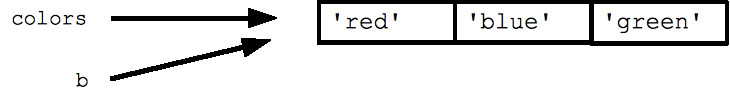
\includegraphics[width=4.16in,height=1.5in]{./uploads_new/SENDING_EMAIL.docx_DIR/media/image2.gif}
			\end{center}
		\end{figure}
		
		
		%%%%%%%%%%%%  Figure/Image No:2 Ends Here %%%%%%%%%%%%%%
		
		
	\end{center}\vspace{12pt}
	\noindent 
	\begin{center}Gambar proses cara kerja mail server 1\end{center} \par
	\vspace{12pt}
	\noindent 
	\begin{center}
		
		%%%%%%%%%%%%  Figure/Image No:3 here %%%%%%%%%%%%%%
		
		
		\begin{figure}[H]
			\begin{center}
				\includegraphics[width=3.97in,height=3.26in]{./uploads_new/SENDING_EMAIL.docx_DIR/media/image3.jpg}
			\end{center}
		\end{figure}
		
		
		%%%%%%%%%%%%  Figure/Image No:3 Ends Here %%%%%%%%%%%%%%
		
		
	\end{center}\vspace{12pt}
	\noindent 
	\begin{center}Gambar proses cara kerja mail server 2\end{center} \par
	\vspace{12pt}
	\vspace{12pt}
	\noindent 
	\textbf{Gambar proses cara kerja mail server 1} \par
	\noindent 
	\textbf{Cara Kerja Mail Server  $  \#  $Versi 2} \par
	Cara kerja ini saya ambil dari Xmodulo, sebelum memahami proses cara kerja mail server sebaiknya anda mengenal terlebih dahulu singkatan - singkatan dari MUA, MTA, MDA dll. Berikut penjelasannya : \par
	\vspace{12pt}
	\noindent 
	\begin{myEnumerate}
		\item Mail User Agent (MUA) : MUA adalah komponen yang berinteraksi dengan pengguna akhir secara langsung. Contoh dari MUA yaitu Thunderbird, MS Outlook, Zimbra Desktop. Interface webmail seperti Gmail dan Yahoo juga MUA. \par
		\noindent 
		\item Mail Transfer Agent (MTA) : MTA bertanggung jawab untuk mentransfer email dari mail server mengirimkan sampai ke server penerima email. Contoh MTA yaitu sendmail dan postfix. \par
		\noindent 
		\item Mail Delivery Agent (MDA) : Dalam surat server tujuan, MTA lokal menerima email masuk dari MTA terpencil. Email tersebut kemudian dikirimkan ke kotak surat pengguna dengan MDA. \par
		\noindent 
		\item POP / IMAP : POP dan IMAP adalah protokol yang digunakan untuk mengambil email dari kotak surat penerima server untuk penerima MUA. \par
		\noindent 
		\item Mail Exchanger Record (MX) : Record MX adalah entri DNS untuk mail server. Catatan ini menunjuk ke alamat IP ke arah mana email harus ditembak. MX record terendah selalu menang, yaitu, mendapat prioritas tertinggi. Sebagai contoh, MX 10 adalah lebih baik daripada MX 20. Alamat IP dari MX record dapat bervariasi berdasarkan desain dan konfigurasi persyaratan, seperti yang akan dibahas nanti dalam artikel.\end{myEnumerate}
	\par
	\vspace{12pt}
	\noindent 
	\begin{center}
		
		%%%%%%%%%%%%  Figure/Image No:4 here %%%%%%%%%%%%%%
		
		
		\begin{figure}[H]
			\begin{center}
				\includegraphics[width=6.27in,height=2.16in]{./uploads_new/SENDING_EMAIL.docx_DIR/media/image4.jpg}
			\end{center}
		\end{figure}
		
		
		%%%%%%%%%%%%  Figure/Image No:4 Ends Here %%%%%%%%%%%%%%
		
		
	\end{center}\vspace{12pt}
	Ketika pengirim mengklik tombol kirim, SMTP (MTA) memastikan ujung ke ujung pengiriman email dari pengirim-sisi server ke server tujuan. Setelah mencapai server tujuan, MTA lokal ke server tujuan menerima email, dan di pindahkan ke MDA setempat. MDA kemudian menulis email ke kotak pesan penerima. Ketika penerima memeriksa email, mereka diambil oleh MUA dengan menggunakan protokol seperti POP atau IMAP. \par
	\vspace{12pt}

\chapter[Python Multithread Programming]
{Python Multithread Programming}
\\}\end{center} \par
\vspace{14pt}
\vspace{14pt}
Menjalankan beberapa\textit{ thread} mirip dengan menjalankan beberapa program yang berbeda secara bersamaan, namun dengan manfaat berikut : \par
\begin{itemize}
\item Beberapa \textit{thread} dalam proses berbagi ruang data yang sama dengan benang induk dan karena dapat saling berbagi informasi atau berkomunikasi satu sama lain dengan lebih muda daripada jika prosesnya terpisah \par
\item \textit{thread} terkadang disebut proses ringan dan tidak membutuhkan banyak memori atas, mereka lebih murah daripada proses.\end{itemize}
\par
Sebuah \textit{thread} memiliki permulaan, urutan eksekusi dan sebuah kesimpulan. Ini memiliki pointer perintah yang melacak dari mana dalam konteksnya saat ini berjalan.  \par
\noindent 
\begin{itemize}
\item Hal ini dapat dilakukan sebelum pre-\textit{empted} (\textit{inturrepted}) \par
\noindent 
\item Untuk sementara dapat ditunda sementara \textit{thread} lainnya yang sedang berjalan ini disebut unggul. \end{itemize}
\par
\noindent 

\section{Memulai Thread Baru}
\\}\end{center \par
\noindent 
\hspace*{0.5in} Untuk melakukan \textit{thread} lain, perlu memanggil metode berikut yang tersedia dimodul \textit{thread} : \par
\noindent 
\begin{center}{\fontsize{9pt}{9pt}\selectfont Thread.start $  \_  $new $  \_  $thread (function, args [, kwargs] )}\end{center} \par
\vspace{12pt}
Pemanggilan metode ini memungkinkan cara cepat dan tepat untuk membuat \textit{thread} baru di linux dan window. \par
Pemanggilan metode segera kembali dan anak  \textit{thread} dimulai dan fungsi pemanggilan dengan daftar \textit{args} telah berlalu. Saat fungsi kembali ujung \textit{thread} akan berakhir.   \par
Disini, \textit{args }adalah tupel argumen. Gunakan tupel kosong untuk memanggil fungsi tanpa melewati argumen. \textit{Kwargs} adalah kamus opsional argumen kata kunci.  \par
\noindent 
\par
\noindent 
Contoh : \par
\noindent 
{\fontsize{10pt}{10pt}\selectfont  $  \#  $!/usr/bin/python} \par
\vspace{10pt}
\noindent 
{\fontsize{10pt}{10pt}\selectfont Import thread} \par
\noindent 
{\fontsize{10pt}{10pt}\selectfont Import time} \par
\vspace{10pt}
\noindent 
{\fontsize{10pt}{10pt}\selectfont  $  \#  $ Define a function for the thread} \par
\noindent 
{\fontsize{10pt}{10pt}\selectfont Def print $  \_  $time (threadNamw, delay):} \par
\noindent 
{\fontsize{10pt}{10pt}\selectfont  \hspace*{0.5in} Count = 0} \par
\noindent 
{\fontsize{10pt}{10pt}\selectfont  \hspace*{0.5in} While count <5:} \par
\noindent 
{\fontsize{10pt}{10pt}\selectfont  \hspace*{0.5in} Time.sleep(delay)} \par
\noindent 
{\fontsize{10pt}{10pt}\selectfont  \hspace*{0.5in} Count +=1} \par
\noindent 
{\fontsize{10pt}{10pt}\selectfont  \hspace*{0.5in} Print  $ " $ $  \%  $s :  $  \%  $s $ " $  $  \%  $ (threadName, time.ctime(time.time()))} \par
\vspace{10pt}
\noindent 
{\fontsize{10pt}{10pt}\selectfont  $  \#  $ Create two thread as follows} \par
\noindent 
{\fontsize{10pt}{10pt}\selectfont try:} \par
\noindent 
{\fontsize{10pt}{10pt}\selectfont  thread.start $  \_  $new $  \_  $thread(print $  \_  $time, ( $ " $Thread-1 $ " $, 2, ))} \par
\noindent 
{\fontsize{10pt}{10pt}\selectfont  thread.start $  \_  $new $  \_  $thread(print $  \_  $time, ( $ " $Thread-2 $ " $, 4,))} \par
\noindent 
{\fontsize{10pt}{10pt}\selectfont except:} \par
\noindent 
{\fontsize{10pt}{10pt}\selectfont ~~ print  $ " $Error: unable to start thread $ " $} \par
\vspace{10pt}
\noindent 
{\fontsize{10pt}{10pt}\selectfont while 1:} \par
\noindent 
{\fontsize{10pt}{10pt}\selectfont pass} \par
\noindent 
~~~~~~ Bila kode diatas dieksekusi, maka menghasilkan hasil sebagai berikut : \par
\noindent 
\begin{center}{\fontsize{10pt}{10pt}\selectfont Thread-1 : Thu Jan 22 15:42:17 2009}\end{center} \par
\noindent 
\begin{center}{\fontsize{10pt}{10pt}\selectfont Thread-1 : Thu Jan 22 15:42:19 2009}\end{center} \par
\noindent 
\begin{center}{\fontsize{10pt}{10pt}\selectfont Thread-2 : Thu Jan 22 15:42:19 2009}\end{center} \par
\noindent 
\begin{center}{\fontsize{10pt}{10pt}\selectfont Thread-1 : Thu Jan 22 15:42:21 2009}\end{center} \par
\noindent 
\begin{center}{\fontsize{10pt}{10pt}\selectfont Thread-2 : Thu Jan 22 15:42:23 2009}\end{center} \par
\noindent 
\begin{center}{\fontsize{10pt}{10pt}\selectfont Thread-1 : Thu Jan 22 15:42:23 2009}\end{center} \par
\noindent 
\begin{center}{\fontsize{10pt}{10pt}\selectfont Thread-1~:  Thu Jan 22 15:42:23 2009}\end{center} \par
\noindent 
\begin{center}{\fontsize{10pt}{10pt}\selectfont Thread-1 : Thu Jan 22 15:42:25 2009}\end{center} \par
\noindent 
\begin{center}{\fontsize{10pt}{10pt}\selectfont Thread-2 : Thu Jan 22 15:42:27 2009}\end{center} \par
\noindent 
\begin{center}{\fontsize{10pt}{10pt}\selectfont Thread-2 : Thu Jan 22 15:42:31 2009}\end{center} \par
\noindent 
\begin{center}{\fontsize{10pt}{10pt}\selectfont Thread-2 : Thu Jan 22 15:42:35 2009}\end{center} \par
\vspace{12pt}
Meskipun sangat efektif untuk benang tingkat rendah, namun modul \textit{thread} sangat terbatas dibandingkan dengan modul yang baru. \par
\vspace{12pt}
\section{Modul Threading }
\\}\end{center} \par
Modul threading yang lebih baru disertakan dengan Python 2.4 memberikan jauh lebih kuat, dukungan tingkat tinggi untuk \textit{thread}\textit{ }dari modul\textit{ }\textit{thread}\textit{ }dibahas pada bagian sebelumnya. \par
The \textit{thread}\textit{ing }modul mengekpos semua metode dari \textit{thread}\textit{ }dan menyediakan beberapa metode tambahan : \par
\begin{itemize}
	\item \textbf{t}\textbf{hreading.activeCount() } \par
	Mengembalikan jumlah objek \textit{thread} yang aktif \par
	\item \textbf{t}\textbf{hreading.currentThread() } \par
	Mengembalikan jumlah objek \textit{thread} dalam kontrol benang pemanggil \par
	\item \textbf{t}\textbf{hreading.enumerate() } \par
	Mengembalikan daftar semua benda \textit{thread}\textit{ }yang sedang aktif \par
	\vspace{12pt}
	Selain metode, modul \textit{thread}\textit{ing }memiliki \textit{thread}\textit{ }kelas yang mengimplementasikan \textit{thread}\textit{ing. }Metode yang disediakan oleh \textit{thread}\textit{ }kelas adalah sebagai berikut : \par
	\item \textbf{run()} \par
	Metode adalah titik masuk untuk \textit{thread} \par
	\item \textbf{start()} \par
	Metode dimulai\textbf{ }\textit{thread}\textit{ }dengan memanggil metode run \par
	\item \textbf{join(}\textbf{[time]}\textbf{)} \par
	Menunggu benang untuk mengakhiri \par
	\item \textbf{isAlive()} \par
	Metode memeriksa apakah\textbf{ }\textit{thread}\textit{ }masih mengeksekusi\textbf{ } \par
	\item \textbf{getName()} \par
	Metode mengambalikan nama\textbf{ }\textit{thread} \par
	\item \textbf{setName()} \par
	Metode menetapkan nama\textbf{ }\textit{thread} \par
	\vspace{12pt}
\section{Membuat Thread Menggunakan Threading Modul}
\\}\end{center} \par
Untuk melaksanakan \textit{thread}\textit{ }baru menggunakan\textit{ threading} harus melakukan hal berikut : \par
\item \textbf Mendefinisikan subclass dari \textit{thread} kelas \par
\item Menimpa  $  \_  $init $  \_  $ (self [args]) metode untuk menambahkan argumen tambahan \par
\item Menimpa run(self[args]) metode untuk menerapkan apa \textit{thread} harus dilakukan ketika mulai \end{itemize}
\par
\begin{adjustwidth}
Setelah membuat baru \textit{thread} subclass, dapat membuah seuah instance dari itu dan kemudian memulai \textit{thread} baru dengan menerapkan \textit{start(),} yang ada gilirinnya panggilan \textit{run()} metode.\end{adjustwidth}
\par
\vspace{12pt}
\begin{adjustwidth}
Contoh :\end{adjustwidth}
\par
\noindent 
{\fontsize{10pt}{10pt}\selectfont  $  \#  $!/usr/bin/python} \par
\vspace{10pt}
\noindent 
{\fontsize{10pt}{10pt}\selectfont import threading} \par
\noindent 
{\fontsize{10pt}{10pt}\selectfont import time} \par
\vspace{10pt}
\noindent 
{\fontsize{10pt}{10pt}\selectfont exitFlag = 0} \par
\vspace{10pt}
\noindent 
{\fontsize{10pt}{10pt}\selectfont class myThread (threading.Thread):} \par
\noindent 
{\fontsize{10pt}{10pt}\selectfont  \hspace*{0.5in} def $  \_  $init $  \_  $(self, threadID, name, counter) :} \par
\noindent 
{\fontsize{10pt}{10pt}\selectfont ~~~~~~ threading.Thread. $  \_  $init $  \_  $(self)} \par
\noindent 
{\fontsize{10pt}{10pt}\selectfont  \hspace*{0.5in} self.threadID = threadID} \par
\noindent 
{\fontsize{10pt}{10pt}\selectfont  \hspace*{0.5in} self.name = name} \par
\vspace{10pt}
\vspace{10pt}
\vspace{10pt}
\noindent 


%%%%%%%%%%%%  Start New Page here %%%%%%%%%%%%%%


\newpage

{\fontsize{9pt}{9pt}\selectfont self.counter = counter} \par
\noindent 
{\fontsize{9pt}{9pt}\selectfont def run (self) :} \par
\noindent 
{\fontsize{9pt}{9pt}\selectfont  \hspace*{0.5in} print  $ " $Starting  $ " $ + self.name} \par
\noindent 
{\fontsize{9pt}{9pt}\selectfont  \hspace*{0.5in} print $  \_  $time(self.name, self.counter, 5)} \par
\noindent 
{\fontsize{9pt}{9pt}\selectfont  \hspace*{0.5in} print  $ " $Exiting  $ " $+ self.name} \par
\vspace{9pt}
\noindent 
{\fontsize{9pt}{9pt}\selectfont def print $  \_  $time(threadName, delay, counter):} \par
\noindent 
{\fontsize{9pt}{9pt}\selectfont while counter:} \par
\noindent 
{\fontsize{9pt}{9pt}\selectfont  \hspace*{0.5in} if exitFlag:} \par
\noindent 
{\fontsize{9pt}{9pt}\selectfont  \hspace*{0.5in}  \hspace*{0.5in} threadName.exit()} \par
\noindent 
{\fontsize{9pt}{9pt}\selectfont  \hspace*{0.5in} time.sleep(delay)} \par
\noindent 
{\fontsize{9pt}{9pt}\selectfont  \hspace*{0.5in} print  $ " $ $  \%  $s:  $  \%  $s $ " $  $  \%  $ (threadName, time.ctime(time.time()))} \par
\noindent 
{\fontsize{9pt}{9pt}\selectfont counter -= 1} \par
\vspace{9pt}
\noindent 
{\fontsize{9pt}{9pt}\selectfont  $  \#  $ Create new threads} \par
\noindent 
{\fontsize{9pt}{9pt}\selectfont thread1 = myThread(1,  $ " $Thread-1 $ " $, 1)} \par
\noindent 
{\fontsize{9pt}{9pt}\selectfont thread2 = myThread(2,  $ " $Thread-2 $ " $, 2)} \par
\vspace{9pt}
\noindent 
{\fontsize{9pt}{9pt}\selectfont  $  \#  $ Start new threads} \par
\noindent 
{\fontsize{9pt}{9pt}\selectfont thread1.start()} \par
\noindent 
{\fontsize{9pt}{9pt}\selectfont thread2.start()} \par
\noindent 
{\fontsize{9pt}{9pt}\selectfont print  $ " $Exiting Main Thread $ " $} \par
\vspace{12pt}
\begin{adjustwidth}
Ketika kode diatas dijalankan, menghasilkan hasil sebagai berikut:\end{adjustwidth}
\par
\noindent 
{\fontsize{10pt}{10pt}\selectfont Starting Thread-1} \par
\noindent 
{\fontsize{10pt}{10pt}\selectfont Starting Thread-2} \par
\noindent 
{\fontsize{10pt}{10pt}\selectfont Exiting Main Thread} \par
\noindent 
{\fontsize{10pt}{10pt}\selectfont Thread-1 : Thu Mar 21 09:10:03 2013} \par
\noindent 
{\fontsize{10pt}{10pt}\selectfont Thread-1 : Thu Mar 21 09:10:04 2013} \par
\noindent 
{\fontsize{10pt}{10pt}\selectfont Thread-2 : Thu Mar 21 09:10:04 2013} \par
\noindent 
{\fontsize{10pt}{10pt}\selectfont Thread-1 : Thu Mar 21 09:10:05 2013} \par
\noindent 
{\fontsize{10pt}{10pt}\selectfont Thread-2 : Thu Mar 21 09:10:06 2013} \par
\noindent 
{\fontsize{10pt}{10pt}\selectfont Thread-1 : Thu Mar 21 09:10:07 2013} \par
\noindent 
{\fontsize{10pt}{10pt}\selectfont Exiting Thread-1} \par
\noindent 
{\fontsize{10pt}{10pt}\selectfont Thread-2 : Thu Mar 21 09:10:08 2013} \par
\noindent 
{\fontsize{10pt}{10pt}\selectfont Thread-2 : Thu Mar 21 09:10:10 2013} \par
\noindent 
{\fontsize{10pt}{10pt}\selectfont Thread-2 : Thu Mar 21 09:10:12 2013} \par
\noindent 
{\fontsize{10pt}{10pt}\selectfont Exiting Thread=2} \par
\vspace{12pt}
\section{Sinkronisasi Thread}
\\}\end{center} \par
{T}\textit{hread}\textit{ing }modul disediakan dengan Python termasuk sederhana untuk menerapkan mekanisme bahwa memungkinkan untuk menyinkronkan \textit{thread}\textit{ }penguncian. Sebuah kunci baru dibuat dengan memanggil \textit{lock() }metode yang mengembalikan kunci baru. \par
The \textit{acquire}\textit{ }\textit{(blocking)}\textit{ }metode objek kunci baru digunakan untuk memaksa \textit{thread}\textit{ }untuk menjalankan serempak. Opsional \textit{blocking} parameter memungkikan untuk mengontrol apakah\textit{ thread} menunggu untuk mendapatkan kunci. \par
Jika \textit{blocking} diatur ke 0, \textit{thread} segera kembali dengan nilai 0 jika kunci tidak dapat diperoleh dan dengan 1 jika kunci dikuisisi. Jika pemblokiran diatur ke 1, blok dan menunggu kunci yang akan dirilis. \par
The \textit{release()} metode objek kunci baru digunakan untuk melepaskan kunci ketika tidak lagi diperlukan.  \par
Contoh: \par
\noindent 
{\fontsize{10pt}{10pt}\selectfont  $  \#  $!/usr/bin/python} \par
\vspace{10pt}
\noindent 
{\fontsize{10pt}{10pt}\selectfont import threading} \par
\noindent 
{\fontsize{10pt}{10pt}\selectfont import time} \par
\vspace{10pt}
\noindent 
{\fontsize{10pt}{10pt}\selectfont class myThread (threading.Thread):} \par
\noindent 
{\fontsize{10pt}{10pt}\selectfont ~ def $  \_  $init $  \_  $(self, threadID, name, counter):} \par
\noindent 
{\fontsize{10pt}{10pt}\selectfont ~~~~ threading.Thread. $  \_  $init $  \_  $(self)} \par
\noindent 
{\fontsize{10pt}{10pt}\selectfont ~~~~ self.threadID = threadID} \par
\noindent 
{\fontsize{10pt}{10pt}\selectfont ~~~~ self.name = name} \par
\noindent 
{\fontsize{10pt}{10pt}\selectfont ~~~~ self.counter = counter} \par
\noindent 
{\fontsize{10pt}{10pt}\selectfont ~ def run(self)} \par
\noindent 
{\fontsize{10pt}{10pt}\selectfont ~~~~ print  $ " $Starting  $ " $+ self.name} \par
\noindent 
{\fontsize{10pt}{10pt}\selectfont ~~~~  $  \#  $ Get lock to synchronize threads} \par
\noindent 
{\fontsize{10pt}{10pt}\selectfont ~~~~ ThreadLock.acquire()} \par
\noindent 
{\fontsize{10pt}{10pt}\selectfont ~~~~ print $  \_  $time(self.name, self.counter, 3)} \par
\noindent 
{\fontsize{10pt}{10pt}\selectfont ~~~~  $  \#  $ Free lock to realease next thread} \par
\noindent 
{\fontsize{10pt}{10pt}\selectfont ~~~~ ThreadLock.release()} \par
\noindent 
{\fontsize{10pt}{10pt}\selectfont ~ } \par
\noindent 
{\fontsize{10pt}{10pt}\selectfont ~ Def print $  \_  $time(threadName, delay, counter):} \par
\noindent 
{\fontsize{10pt}{10pt}\selectfont ~~ while counter:} \par
\noindent 
{\fontsize{10pt}{10pt}\selectfont ~~~ time.sleep(delay)} \par
\noindent 
{\fontsize{10pt}{10pt}\selectfont ~~~ print  $ " $ $  \%  $s:  $  \%  $s $ " $  $  \%  $ (threadName, time.ctime(time.time()))} \par
\noindent 
{\fontsize{10pt}{10pt}\selectfont ~~~ counter -= 1} \par
\noindent 
{\fontsize{10pt}{10pt}\selectfont ~ threadLock = threading.Lock()} \par
\noindent 
{\fontsize{10pt}{10pt}\selectfont ~ threads = []} \par
\vspace{10pt}
\noindent 
{\fontsize{10pt}{10pt}\selectfont  $  \#  $ Create new threads} \par
\noindent 
{\fontsize{10pt}{10pt}\selectfont thread1 = myThread(1,  $ " $Thread-1,1 )} \par
\noindent 
{\fontsize{10pt}{10pt}\selectfont thread2 = myThread(2,  $ " $Thread-2,2 )} \par
\vspace{10pt}
\noindent 
{\fontsize{10pt}{10pt}\selectfont  $  \#  $ Start new Threads} \par
\noindent 
{\fontsize{10pt}{10pt}\selectfont thread1.start()} \par
\noindent 
{\fontsize{10pt}{10pt}\selectfont thread2.start()} \par
\vspace{10pt}
\noindent 
{\fontsize{10pt}{10pt}\selectfont  $  \#  $ Add threads to thread list} \par
\noindent 
{\fontsize{10pt}{10pt}\selectfont threads.append(thread1)} \par
\noindent 
{\fontsize{10pt}{10pt}\selectfont thread2.append(thread2)} \par
\vspace{10pt}
\noindent 
{\fontsize{10pt}{10pt}\selectfont  $  \#  $ Wait for all threads to complete} \par
\noindent 
{\fontsize{10pt}{10pt}\selectfont Fort t in threads:} \par
\noindent 
{\fontsize{10pt}{10pt}\selectfont ~~~~ t.join()} \par
\noindent 
{\fontsize{10pt}{10pt}\selectfont print  $ " $Exiting Main thread $ " $} \par
\vspace{10pt}
\noindent 
Bila kode diatas dieksekusi, maka menghasilkan sebagai berikut : \par
\vspace{10pt}
\noindent 
{\fontsize{10pt}{10pt}\selectfont Starting Thread-1} \par
\noindent 
{\fontsize{10pt}{10pt}\selectfont Starting Thread-2} \par
\noindent 
{\fontsize{10pt}{10pt}\selectfont Thread-1: Thu Mar 21 09:11:28 2013} \par
\noindent 
{\fontsize{10pt}{10pt}\selectfont Thread-1: Thu Mar 21 09:11:29 2013} \par
\noindent 
{\fontsize{10pt}{10pt}\selectfont Thread-1: Thu Mar 21 09:11:30 2013} \par
\noindent 
{\fontsize{10pt}{10pt}\selectfont Thread-2: Thu Mar 21 09:11:32 2013} \par
\noindent 
{\fontsize{10pt}{10pt}\selectfont Thread-2: Thu Mar 21 09:11:34 2013} \par
\noindent 
{\fontsize{10pt}{10pt}\selectfont Thread-2: Thu Mar 21 09:11:36 2013} \par
\noindent 
{\fontsize{10pt}{10pt}\selectfont Exiting Main Thread} \par
\vspace{12pt}
\section{Multithreaded Antrian Prioritas}
\\}\end{center} \par
The queue modul memungkinkan untuk membuat objek antrian baru yang dapat menampung jumlah tertentu item. Ada metode berikut untuk mengontrol antrian : \par
\begin{itemize}
	\item \textbf{get()} \par
	\begin{adjustwidth}
		Menghapus dan mengembalikan item dari antrian\end{adjustwidth}
	\par
	\item \textbf{put()} \par
	\begin{adjustwidth}
		Menambahkan item ke antrian\end{adjustwidth}
	\par
	\item \textbf{qsize()} \par
	\begin{adjustwidth}
		Mengembalikan jumlah item yang saat ini dalam antrian\end{adjustwidth}
	\par
	\item \textbf{empty()} \par
	\begin{adjustwidth}
		Mengembalikan benar jika antrian kosong jika tidak, salah\end{adjustwidth}
	\par
	\item \textbf{full()}\end{itemize}
\par
\begin{adjustwidth}
	Mengembalikan benar jika antrian penuh jika tidak, salah\end{adjustwidth}
\par
Contoh: \par
\noindent 
{\fontsize{10pt}{10pt}\selectfont  $  \#  $!/usr/bin/python} \par
\vspace{10pt}
\noindent 
{\fontsize{10pt}{10pt}\selectfont import Queue} \par
\noindent 
{\fontsize{10pt}{10pt}\selectfont import threading} \par
\noindent 
{\fontsize{10pt}{10pt}\selectfont import time} \par
\vspace{10pt}
\noindent 
{\fontsize{10pt}{10pt}\selectfont exitFlag = 0} \par
\vspace{10pt}
\noindent 
{\fontsize{10pt}{10pt}\selectfont class myThread (threading.Thread):} \par
\noindent 
{\fontsize{10pt}{10pt}\selectfont ~~def   $  \_  $init $  \_  $(self, threadID, name, q):} \par
\noindent 
{\fontsize{10pt}{10pt}\selectfont ~~~~ threading.Thread. $  \_  $init $  \_  $(self)} \par
\noindent 
{\fontsize{10pt}{10pt}\selectfont ~~~ self.name = name} \par
\noindent 
{\fontsize{10pt}{10pt}\selectfont ~~~ self.q = q} \par
\noindent 
{\fontsize{10pt}{10pt}\selectfont  def run(self):} \par
\noindent 
{\fontsize{10pt}{10pt}\selectfont ~~~~~ print  $ " $Starting  $ " $+ self.name} \par
\noindent 
{\fontsize{10pt}{10pt}\selectfont ~~~~~ process $  \_  $data(self.name, self.q)} \par
\noindent 
{\fontsize{10pt}{10pt}\selectfont ~~~~~ print  $ " $Exiting  $ " $+ self.name} \par
\vspace{10pt}
\noindent 
{\fontsize{10pt}{10pt}\selectfont def process $  \_  $data(threadName, q):} \par
\noindent 
{\fontsize{10pt}{10pt}\selectfont ~~~ while not exitFlag:} \par
\noindent 
{\fontsize{10pt}{10pt}\selectfont ~~~ queuLock.acquire()} \par
\noindent 
{\fontsize{10pt}{10pt}\selectfont ~~~ if not workQueu.empty():} \par
\noindent 
{\fontsize{10pt}{10pt}\selectfont ~~~~~~~ data = q.get()} \par
\noindent 
{\fontsize{10pt}{10pt}\selectfont ~~~~~~~ queueLock.release()} \par
\noindent 
{\fontsize{10pt}{10pt}\selectfont ~~~~~~~ print  $ " $ $  \%  $s processing  $  \%  $s $ " $  $  \%  $ (threadName, data)} \par
\noindent 
{\fontsize{10pt}{10pt}\selectfont ~~~~ else:} \par
\noindent 
{\fontsize{10pt}{10pt}\selectfont ~~~~~~~ queueLock.release()} \par
\noindent 
{\fontsize{10pt}{10pt}\selectfont ~~~~~~~ time.sleep(1)} \par
\vspace{12pt}
\noindent 
{\fontsize{10pt}{10pt}\selectfont threadList = [ $ " $Thread-1 $ " $,  $ " $Thread-2 $ " $,  $ " $Thread-3 $ " $]} \par
\noindent 
{\fontsize{10pt}{10pt}\selectfont nameList = [ $ " $One $ " $,  $ " $Two $ " $,  $ " $Three $ " $,  $ " $Four $ " $,  $ " $Five $ " $]} \par
\noindent 
{\fontsize{10pt}{10pt}\selectfont queueLock = threading.Lock()} \par
\noindent 
{\fontsize{10pt}{10pt}\selectfont workLock = Queue.Queue(10)} \par
\noindent 
{\fontsize{10pt}{10pt}\selectfont threads = []} \par
\noindent 
{\fontsize{10pt}{10pt}\selectfont threadID = 1} \par
\vspace{10pt}
\noindent 
{\fontsize{10pt}{10pt}\selectfont  $  \#  $ Create new threads} \par
\noindent 
{\fontsize{10pt}{10pt}\selectfont For tName in threadList:} \par
\noindent 
{\fontsize{10pt}{10pt}\selectfont ~~~ thread = myThread(threadID, tName, workQueue)} \par
\noindent 
{\fontsize{10pt}{10pt}\selectfont ~~~ thread.start()} \par
\noindent 
{\fontsize{10pt}{10pt}\selectfont ~~~ thread.append(thread)} \par
\noindent 
{\fontsize{10pt}{10pt}\selectfont ~~~ threadID +=1} \par
\vspace{10pt}
\noindent 
{\fontsize{10pt}{10pt}\selectfont  $  \#  $ Fill the queue} \par
\noindent 
{\fontsize{10pt}{10pt}\selectfont queueLock.acquire()} \par
\noindent 
{\fontsize{10pt}{10pt}\selectfont for word in nameList:} \par
\noindent 
{\fontsize{10pt}{10pt}\selectfont ~~~ workQueue.put(word)} \par
\noindent 
{\fontsize{10pt}{10pt}\selectfont queueLock.release()} \par
\vspace{10pt}
\noindent 
{\fontsize{10pt}{10pt}\selectfont  $  \#  $ Wait for queue to empty} \par
\noindent 
{\fontsize{10pt}{10pt}\selectfont while not workQueue.empty():} \par
\noindent 
{\fontsize{10pt}{10pt}\selectfont pass} \par
\vspace{10pt}
\noindent 
{\fontsize{10pt}{10pt}\selectfont  $  \#  $ Notify threads it’s time to exit} \par
\noindent 
{\fontsize{10pt}{10pt}\selectfont exitFlag = 1} \par
\vspace{10pt}
\noindent 
{\fontsize{10pt}{10pt}\selectfont  $  \#  $ Wait for all threads to complete} \par
\noindent 
{\fontsize{10pt}{10pt}\selectfont For t in threads:} \par
\noindent 
{\fontsize{10pt}{10pt}\selectfont ~~~ t.join()} \par
\noindent 
{\fontsize{10pt}{10pt}\selectfont print  $ " $Exiting Main Thread $ " $} \par
\vspace{10pt}
\noindent 
Bila kode diatas dieksekusi, maka menghasilkan hasil sebagai berikut: \par
\vspace{12pt}
\noindent 
{\fontsize{10pt}{10pt}\selectfont Starting Thread-1} \par
\noindent 
{\fontsize{10pt}{10pt}\selectfont Starting Thread-2} \par
\noindent 
{\fontsize{10pt}{10pt}\selectfont Starting Thread-3} \par
\noindent 
{\fontsize{10pt}{10pt}\selectfont Thread-1 processing One} \par
\noindent 
{\fontsize{10pt}{10pt}\selectfont Thread-2 processing Two} \par
\noindent 
{\fontsize{10pt}{10pt}\selectfont Thread-3 processing Three} \par
\noindent 
{\fontsize{10pt}{10pt}\selectfont Thread-1 processing Four} \par
\noindent 
{\fontsize{10pt}{10pt}\selectfont Thread-2 processing Five} \par
\noindent 
{\fontsize{10pt}{10pt}\selectfont Exiting Thread-3} \par
\noindent 
{\fontsize{10pt}{10pt}\selectfont Exiting Thread-1} \par
\noindent 
{\fontsize{10pt}{10pt}\selectfont Exiting Thread-2} \par
\noindent 
{\fontsize{10pt}{10pt}\selectfont Exiting Main Thread} \par
\noindent 
\vspace{40pt}

\chapter{XML Processing}
XML adalah bahasa open source portable yang memungkinkan pemrogram mengemangkan aplikasi yang dapat dibaca oleh aplikasi lain, terlepas dari sistem operasi dan bahasa pengembangnya. \par
\vspace{12pt}
\noindent 
Apa itu XML? \par
Extensible Markup Languange (XML) adalah bahasa markup seperti HTML atau SGML. Ini direkomendasikan oleh World Wide Web Consortium dan tersedia sebagai standar terbuka.  \par
XML sangat berguna untuk mencatat data berukuran kecil dan menengah tanpa memerlukan tulang punggung berbasis SQL. \par
\vspace{12pt}
\noindent 

\section{Arsitektur Parsing XML dan API}
 \par
\noindent 
\hspace*{0.5in} Perpustakaan standar Python menyediakan seperangkat antarmuka minimal tapi berguna untuk bekerja dengan XML.  \par
\noindent 
\hspace*{0.5in} Dua API yang paling dasar dan umum digunakan untuk data XML adalah antarmuka SAX dan DOM. \par
\noindent 
\hspace*{0.5in} API sederhana untuk XML (SAX): mendaftarkan panggilan kemali untuk acara yang diminati dan kemudian membiarkan parser berjalan melalui dokumen. Ini berguna bila dokumen berukuran besar atau memiliki keterbatasan memori, ini memparsing file tidak pernah tersimpan dalam memori. \par
\noindent 
\hspace*{0.5in} API Document Objek Model (DOM): ini adalah rekomendasi World Wide Web Consortium dimana keseluruhan file dibaca ke memori dan disimpan dalam bentuk hierarkies (tree-based) untuk mewakili semua fitur dokumen XML.  \par
\noindent 
\hspace*{0.5in} SAX jelas tidak bisa memproses informasi secepat DOM saat bisa bekerjadengan file besar. Di sisi lain, menggunakan DOM secara eklusifenar-benar dapat membunuh sumber daya, terutama jika digunakan pada banyak file kecil. \par
\noindent 
~~~~~~~~~~~ SAX hanya bisa dibaca sementara DOM mengizinkan perubahan pada file XML. Kedua API yang berbeda ini saling melengkapi satu sama lain, tidak ada alasan mengapa tidak dapat menggunakannya untuk proyek besar. \par
\noindent 


\vspace{12pt}
\vspace{12pt}
\noindent 
Contoh: \par
\noindent 
<collection shelf="New Arrivals"> \par
\noindent 
<movie title="Enemy Behind"> \par
\noindent 
~~ <type>War, Thriller</type> \par
\noindent 
~~ <format>DVD</format> \par
\noindent 
~~ <year>2003</year> \par
\noindent 
~~ <rating>PG</rating> \par
\noindent 
~~ <stars>10</stars> \par
\noindent 
~~ <description>Talk about a US-Japan war</description> \par
\noindent 
</movie> \par
\noindent 
<movie title="Transformers"> \par
\noindent 
~~ <type>Anime, Science Fiction</type> \par
\noindent 
~~ <format>DVD</format> \par
\noindent 
~~ <year>1989</year> \par
\noindent 
~~ <rating>R</rating> \par
\noindent 
~~ <stars>8</stars> \par
\noindent 
~~ <description>A schientific fiction</description> \par
\noindent 
</movie> \par
\noindent 
~~ <movie title="Trigun"> \par
\noindent 
~~ <type>Anime, Action</type> \par
\noindent 
~~ <format>DVD</format> \par
\noindent 
~~ <episodes>4</episodes> \par
\noindent 
~~ <rating>PG</rating> \par
\noindent 
~~ <stars>10</stars> \par
\noindent 
~~ <description>Vash the Stampede!</description> \par
\noindent 
</movie> \par
\noindent 
<movie title="Ishtar"> \par
\noindent 
~~ <type>Comedy</type> \par
\noindent 
~~ <format>VHS</format> \par
\noindent 
~~ <rating>PG</rating> \par
\noindent 
~~ <stars>2</stars> \par
\noindent 
~~ <description>Viewable boredom</description> \par
\noindent 
</movie> \par
\noindent 
</collection> \par
\vspace{10pt}
\noindent

\section{Parsing XML dan API SAX}
\par
\noindent 
\hspace*{0.5in} SAX adalah antarmuka standar untuk parsing XML berbasis event. Parsing XML dengan SAX umumnya mengharuskan untuk membuat C\textit{ontrolHandler }dengan subclassing xml.sax \textit{controlhandler}. \par
\noindent 
\hspace*{0.5in} \textit{ControlHandler }menangani tag dan atribut tertentu dari XML. Objek \textit{ControlHandler }menyediakan metode untuk menangani berbagai aktivitas parsing. Parsing memanggil metode \textit{ControlHandler }saat memparsing file XML. \par
\noindent 
\hspace*{0.5in} Metode \textit{startDocument} dan \textit{endDocument} disebut awal dan akhir setiap elemen. Jika parsing tidak dalam mode namespace, metode \textit{startElement} (tag attribute) dan \textit{endElement} (tag) dipanggil. Jika tidak, metode yang sesuai \textit{startElemenNS} dan \textit{endElemenNS} dipanggil. Disini, tah adalah tag elemen dan atriut adalah atribut.  \par
\noindent 
\hspace*{0.5in} Berikut ini metode penting untuk memahami sebelum melanjutkan ke materi berikutnya : \par
\noindent 
\begin{myEnumerate}
	\item Metode \textit{make $  \_  $parser} \par
	Metode berikut membuat objek parsing baru dan mengembalikannya. Objek parsing diuat akan menjadi tipe parsing pertama yang ditemukan sistem.  \par
	\vspace{10pt}
	{\fontsize{10pt}{10pt}\selectfont xml.sax.make $  \_  $parser([parser $  \_  $list])} \par
	\vspace{12pt}
	Berikut adalah detail parameternya : \par
	Parser $  \_  $list : pilihan argumen yang terdiri dari daftar parsing untuk digunakan yang semuanya harus menerapkan metode \textit{make $  \_  $parse} \par
	\noindent 
	\item Metode \textit{parser} \par
	Metode berikut membuat parsing SAX dan menggunakannya untuk mengurai dokumen \par
	\vspace{10pt}
	{\fontsize{10pt}{10pt}\selectfont xml.sax.parser(xmlfile, contenthandler[, errorhandler])} \par
	\vspace{10pt}
	Berikut adalah detail dari parameternya: \par
	\noindent 
	\begin{itemize}
		\item \textit{Xmlfile } \par
		Ini adalah nama file XML yang bisa dibaca. \par
		\noindent 
		\item \textit{ContentHandler } \par
		Ini harus menjadi objek \textit{ContenHandler} \par
		\noindent 
		\item \textit{ErrorHandler} \par
		Jika ditentukan, e\textit{rrorhandler} harus menjadi objek \textit{ErrorHandler} SAX \par
		\noindent 
		\item Metode\textit{ parseString}\end{itemize}
	\par
	Membuat parsing SAX dan mengurai string XML yang ditentukan : \par
	\vspace{12pt}
	{\fontsize{10pt}{10pt}\selectfont xml.sax.parsertring(xmlstring,contenthandler[, errorhandler])} \par
	\vspace{12pt}
	Brikut ini adalah detail nama dar parameter : \par
	\noindent 
	\item \textit{XMLstring} \par
	Nama dari string yang bisa dibaca \par
	\noindent 
	\item \textit{ContentHandler} \par
	Menjadi objek ContenHandler \par
	\noindent 
	\item \textit{ErrorHandler} \par
	Menjadi objek ErorHandler SAX \par
	\vspace{12pt}
	\noindent 
	Contoh : \par
	\noindent 
	$  \#  $!/usr/bin/python \par
	\vspace{12pt}
	\noindent 
	import xml.sax \par
	\vspace{12pt}
	\noindent 
	class MovieHandler( xml.sax.ContentHandler ): \par
	\noindent 
	~~ def  $  \_  $ $  \_  $init $  \_  $ $  \_  $(self): \par
	\noindent 
	~~~~~ self.CurrentData = "" \par
	\noindent 
	~~~~~ self.type = "" \par
	\noindent 
	~~~~~ self.format = "" \par
	\noindent 
	~~~~~ self.year = "" \par
	\noindent 
	~~~~~ self.rating = "" \par
	\noindent 
	~~~~~ self.stars = "" \par
	\noindent 
	~~~~~ self.description = "" \par
	\vspace{12pt}
	\noindent 
	~~  $  \#  $ Call when an element starts \par
	\noindent 
	~~ def startElement(self, tag, attributes): \par
	\noindent 
	~~~~~ self.CurrentData = tag \par
	\noindent 
	~~~~~ if tag == "movie": \par
	\noindent 
	~~~~~~~~ print "*****Movie*****" \par
	\noindent 
	~~~~~~~~ title = attributes["title"] \par
	\noindent 
	~~~~~~~~ print "Title:", title \par
	\vspace{12pt}
	\noindent 
	~~  $  \#  $ Call when an elements ends \par
	\noindent 
	~~ def endElement(self, tag): \par
	\noindent 
	~~~~~ if self.CurrentData == "type": \par
	\noindent 
	~~~~~~~~ print "Type:", self.type \par
	\noindent 
	~~~~~ elif self.CurrentData == "format": \par
	\noindent 
	~~~~~~~~ print "Format:", self.format \par
	\noindent 
	~~~~~ elif self.CurrentData == "year": \par
	\noindent 
	~~~~~~~~ print "Year:", self.year \par
	\noindent 
	~~~~~ elif self.CurrentData == "rating": \par
	\noindent 
	~~~~~~~~ print "Rating:", self.rating \par
	\noindent 
	~~~~~ elif self.CurrentData == "stars": \par
	\noindent 
	~~~~~~~~ print "Stars:", self.stars \par
	\noindent 
	~~~~~ elif self.CurrentData == "description": \par
	\noindent 
	~~~~~~~~ print "Description:", self.description \par
	\noindent 
	~~~~~ self.CurrentData = "" \par
	\vspace{12pt}
	\noindent 
	~~  $  \#  $ Call when a character is read \par
	\noindent 
	~~ def characters(self, content): \par
	\noindent 
	~~~~~ if self.CurrentData == "type": \par
	\noindent 
	~~~~~~~~ self.type = content \par
	\noindent 
	~~~~~ elif self.CurrentData == "format": \par
	\noindent 
	~~~~~~~~ self.format = content \par
	\noindent 
	~~~~~ elif self.CurrentData == "year": \par
	\noindent 
	~~~~~~~~ self.year = content \par
	\noindent 
	~~~~~ elif self.CurrentData == "rating": \par
	\noindent 
	~~~~~~~~ self.rating = content \par
	\noindent 
	~~~~~ elif self.CurrentData == "stars": \par
	\noindent 
	~~~~~~~~ self.stars = content \par
	\noindent 
	~~~~~ elif self.CurrentData == "description": \par
	\noindent 
	~~~~~~~~ self.description = content \par
	\noindent 
	~  \par
	\noindent 
	if (  $  \_  $ $  \_  $name $  \_  $ $  \_  $ == " $  \_  $ $  \_  $main $  \_  $ $  \_  $"): \par
	\noindent 
	~~  \par
	\noindent 
	~~  $  \#  $ create an XMLReader \par
	\noindent 
	~~ parser = xml.sax.make $  \_  $parser() \par
	\noindent 
	~~  $  \#  $ turn off namepsaces \par
	\noindent 
	~~ parser.setFeature(xml.sax.handler.feature $  \_  $namespaces, 0) \par
	\vspace{12pt}
	\noindent 
	~~  $  \#  $ override the default ContextHandler \par
	\noindent 
	~~ Handler = MovieHandler() \par
	\noindent 
	~~ parser.setContentHandler( Handler ) \par
	\noindent 
	~~  \par
	\noindent 
	~~ parser.parse("movies.xml") \par
	\vspace{12pt}
	\vspace{12pt}
	\noindent 
	Ini akan menghasilkan hasil sebagai berikut: \par
	\noindent 
	{\fontsize{10pt}{10pt}\selectfont *****Movie******} \par
	\noindent 
	{\fontsize{10pt}{10pt}\selectfont *****Movie*****} \par
	\noindent 
	{\fontsize{10pt}{10pt}\selectfont Title: Enemy Behind} \par
	\noindent 
	{\fontsize{10pt}{10pt}\selectfont Type: War, Thriller} \par
	\noindent 
	{\fontsize{10pt}{10pt}\selectfont Format: DVD} \par
	\noindent 
	{\fontsize{10pt}{10pt}\selectfont Year: 2003} \par
	\noindent 
	{\fontsize{10pt}{10pt}\selectfont Rating: PG} \par
	\noindent 
	{\fontsize{10pt}{10pt}\selectfont Stars: 10} \par
	\noindent 
	{\fontsize{10pt}{10pt}\selectfont Description: Talk about a US-Japan war} \par
	\noindent 
	{\fontsize{10pt}{10pt}\selectfont *****Movie*****} \par
	\noindent 
	{\fontsize{10pt}{10pt}\selectfont Title: Transformers} \par
	\noindent 
	{\fontsize{10pt}{10pt}\selectfont Type: Anime, Science Fiction} \par
	\noindent 
	{\fontsize{10pt}{10pt}\selectfont Format: DVD} \par
	\noindent 
	{\fontsize{10pt}{10pt}\selectfont Year: 1989} \par
	\noindent 
	{\fontsize{10pt}{10pt}\selectfont Rating: R} \par
	\noindent 
	{\fontsize{10pt}{10pt}\selectfont Stars: 8} \par
	\noindent 
	{\fontsize{10pt}{10pt}\selectfont Description: A schientific fiction} \par
	\noindent 
	{\fontsize{10pt}{10pt}\selectfont *****Movie*****} \par
	\noindent 
	{\fontsize{10pt}{10pt}\selectfont Title: Trigun} \par
	\noindent 
	{\fontsize{10pt}{10pt}\selectfont Type: Anime, Action} \par
	\noindent 
	{\fontsize{10pt}{10pt}\selectfont Format: DVD} \par
	\noindent 
	{\fontsize{10pt}{10pt}\selectfont Rating: PG} \par
	\noindent 
	{\fontsize{10pt}{10pt}\selectfont Stars: 10} \par
	\noindent 
	{\fontsize{10pt}{10pt}\selectfont Description: Vash the Stampede!} \par
	\noindent 
	{\fontsize{10pt}{10pt}\selectfont *****Movie*****} \par
	\noindent 
	{\fontsize{10pt}{10pt}\selectfont Title: Ishtar} \par
	\noindent 
	{\fontsize{10pt}{10pt}\selectfont Type: Comedy} \par
	\noindent 
	{\fontsize{10pt}{10pt}\selectfont Format: VHS} \par
	\noindent 
	{\fontsize{10pt}{10pt}\selectfont Rating: PG} \par
	\noindent 
	{\fontsize{10pt}{10pt}\selectfont Stars: 2} \par
	\noindent 
	{\fontsize{10pt}{10pt}\selectfont Description: Viewable boredom} \par
	\noindent 
	{\fontsize{10pt}{10pt}\selectfont 
			
\section{Parsing XML dan API DOM}
\par
\noindent 
\hspace*{0.5in} Document Ovject Model (DOM) adalah API lintas bahasa dari World Wide Web Consortium (W3C) untuk mengakses dan memodifikasi dokumen XML. \par
\noindent 
\hspace*{0.5in} DOM sangat berguna untuk aplikasi akses acak. SAX hanya memungkinkan melihat satu bit dokumen sekaligus. Jika melihat satu elemen SAX, tidak memiliki akses ke yang lain. \par
\noindent 
\hspace*{0.5in} Berikut adalah cara termudah untuk memuat dokumen XML dengan cepat dan membuat objek minidom menggunakan modul xml.dom. Objek minidom menyediakan metode parsing sederhana yang dengan cepat memuat pohon DOM dari file XML. \par
\noindent 
\hspace*{0.5in} Contoh~frase memanggil fungsi  parsing (file [,parsing]) dari objek minidokumen untuk mengurai file XML yang ditunjuk oleh file ke objek pohon DOM. \par
\noindent 
$  \#  $!/usr/bin/python \par
\vspace{12pt}
\noindent 
from xml.dom.minidom import parse \par
\noindent 
import xml.dom.minidom \par
\vspace{12pt}
\noindent 
$  \#  $ Open XML document using minidom parser \par
\noindent 
DOMTree = xml.dom.minidom.parse("movies.xml") \par
\noindent 
collection = DOMTree.documentElement \par
\noindent 
if collection.hasAttribute("shelf"): \par
\noindent 
~~ print "Root element :  $  \%  $s"  $  \%  $ collection.getAttribute("shelf") \par
\vspace{12pt}
\noindent 
$  \#  $ Get all the movies in the collection \par
\noindent 
movies = collection.getElementsByTagName("movie") \par
\vspace{12pt}
\noindent 
$  \#  $ Print detail of each movie. \par
\noindent 
for movie in movies: \par
\noindent 
~~ print "*****Movie*****" \par
\noindent 
~~ if movie.hasAttribute("title"): \par
\noindent 
~~~~~ print "Title:  $  \%  $s"  $  \%  $ movie.getAttribute("title") \par
\vspace{12pt}
\noindent 
~~ type = movie.getElementsByTagName('type')[0] \par
\noindent 
~~ print "Type:  $  \%  $s"  $  \%  $ type.childNodes[0].data \par
\noindent 
~~ format = movie.getElementsByTagName('format')[0] \par
\noindent 
~~ print "Format:  $  \%  $s"  $  \%  $ format.childNodes[0].data \par
\noindent 
~~ rating = movie.getElementsByTagName('rating')[0] \par
\noindent 
~~ print "Rating:  $  \%  $s"  $  \%  $ rating.childNodes[0].data \par
\noindent 
~~ description = movie.getElementsByTagName('description')[0] \par
\noindent 
~~ print "Description:  $  \%  $s"  $  \%  $ description.childNodes[0].data \par
\vspace{12pt}
\noindent 
Ini akan menghasilkan hasil sebagai berikut : \par
\noindent 
Root element : New Arrivals \par
\noindent 
*****Movie***** \par
\noindent 
Title: Enemy Behind \par
\noindent 
Type: War, Thriller \par
\noindent 
Format: DVD \par
\noindent 
Rating: PG \par
\noindent 
Description: Talk about a US-Japan war \par
\noindent 
*****Movie***** \par
\noindent 
Title: Transformers \par
\noindent 
Type: Anime, Science Fiction \par
\noindent 
Format: DVD \par
\noindent 
Rating: R \par
\noindent 
Description: A schientific fiction \par
\noindent 
*****Movie***** \par
\noindent 
Title: Trigun \par
\noindent 
Type: Anime, Action \par
\noindent 
Format: DVD \par
\noindent 
Rating: PG \par
\noindent 
Description: Vash the Stampede! \par
\noindent 
*****Movie***** \par
\noindent 
Title: Ishtar \par
\noindent 
Type: Comedy \par
\noindent 
Format: VHS \par
\noindent 
Rating: PG \par
\noindent 
Description: Viewable boredom \par
\vspace{12pt}
\noindent

\section{Membangun Parsing Document XML menggunakan Python}
\par
\noindent 
\hspace*{0.5in} Python mendukung untuk bekerja dengan berbagai bentuk markup data terstruktur. Selain mengurai xml.etree. \textit{ElementTree} mendukung pembuatan dokumen XML yang terbentuk dengan baik dari objek elemen yang dibangun dalam aplikasi. Kelas elemen digunakakan saat sebuah dokumen diurai untuk mengetahui bagaimana menghasilkan bentuk serial dari isinya kemudian dapat ditulis ke sebuah file.  \par
\vspace{12pt}
\noindent 
\hspace*{0.5in} Untuk membuat instance elemeb gunakan fungsi elemen contructor dan \textit{SubElemen()} pabrik. \par
\noindent 
Import xml.etree.ElementTree as xml \par
\vspace{12pt}
\noindent 
{\fontsize{10pt}{10pt}\selectfont filename =  $ " $/home/abc/Desktop/test $  \_  $xml.xml $ " $} \par
\noindent 
{\fontsize{10pt}{10pt}\selectfont toot = xml.Element( $ " $Users $ " $)} \par
\noindent 
{\fontsize{10pt}{10pt}\selectfont userelement = xml.Element( $ " $user $ " $)} \par
\noindent 
{\fontsize{10pt}{10pt}\selectfont root.append(userelement)} \par
\noindent 
\vspace{10pt}
\noindent 
Bila menjalankan ini, akan menghasilkan sebagai berikut : \par
\noindent 
{\fontsize{10pt}{10pt}\selectfont <Users>} \par
\noindent 
{\fontsize{10pt}{10pt}\selectfont  \hspace*{0.5in} <user>} \par
\noindent 
{\fontsize{10pt}{10pt}\selectfont  \hspace*{0.5in} <user>} \par
\noindent 
{\fontsize{10pt}{10pt}\selectfont </Users>} \par
\vspace{10pt}
\vspace{10pt}
\vspace{10pt}
\noindent 
Tambahkan anak-anak pegguna \par
\vspace{10pt}
\noindent 
{\fontsize{10pt}{10pt}\selectfont Uid = xml.SubElement(userelement,  $ " $uid $ " $)} \par
\noindent 
{\fontsize{10pt}{10pt}\selectfont Uid.text =  $ " $1 $ " $} \par
\vspace{10pt}
\noindent 
{\fontsize{10pt}{10pt}\selectfont FirstName = xml.SubElement(userelement,  $ " $FirstName $ " $)} \par
\noindent 
{\fontsize{10pt}{10pt}\selectfont FirstName.text =  $ " $testuser $ " $} \par
\vspace{10pt}
\noindent 
{\fontsize{10pt}{10pt}\selectfont LastName = xml.SubElement(userelement,  $ " $LastName $ " $} \par
\noindent 
{\fontsize{10pt}{10pt}\selectfont LastName.text =  $ " $testuser $ " $} \par
\vspace{10pt}
\noindent 
{\fontsize{10pt}{10pt}\selectfont Email = xml.SubElement(userelement,  $ " $Email $ " $)} \par
\noindent 
{\fontsize{10pt}{10pt}\selectfont Email.text = \href{mailto:testuser@test.com}{testuser@test.com}
} \par
\vspace{10pt}
\noindent 
{\fontsize{10pt}{10pt}\selectfont state = xml.SubElement(userelemet,  $ " $state $ " $)} \par
\noindent 
{\fontsize{10pt}{10pt}\selectfont state.text =  $ " $xyz $ " $} \par
\vspace{10pt}
\noindent 
{\fontsize{10pt}{10pt}\selectfont location = xml.SubElement(userelement,  $ " $location)} \par
\noindent 
{\fontsize{10pt}{10pt}\selectfont location.text = abc} \par
\vspace{10pt}
\noindent 
{\fontsize{10pt}{10pt}\selectfont tree = xml.ElementTree(root)} \par
\noindent 
{\fontsize{10pt}{10pt}\selectfont with open(filename,  $ " $w $ " $) as fh:} \par
\noindent 
{\fontsize{10pt}{10pt}\selectfont tree.write(fh)} \par
\vspace{10pt}
\noindent 
\hspace*{0.5in} Pertama buat elemen root dengan mengunakan fungsi \textit{ElementTree}. Kemudian membuat elemen pegguna dan menambahkannya ke root. Selanjutnya membuat \textit{SubElement }dengan melewatkan elemen pengguna (userelement) ke \textit{SubElemen} beserta namanya seperto  $ " $FirstName $ " $. Kemudian untuk setiap \textit{SubElement} tetapkan properti teks untuk memberi nilai. Di akhir, membuat \textit{ElementTree} dan menggunakannya untuk menulis XML ke file. \par
\noindent 
\hspace*{0.5in} Jika menjalankan ini akan menjadi sebagai berikut : \par
\noindent 
{\fontsize{10pt}{10pt}\selectfont <users>} \par
\noindent 
{\fontsize{10pt}{10pt}\selectfont  \hspace*{0.5in} <user>} \par
\noindent 
{\fontsize{10pt}{10pt}\selectfont  \hspace*{0.5in}  \hspace*{0.5in} <uid>1</uid>} \par
\noindent 
{\fontsize{10pt}{10pt}\selectfont  \hspace*{0.5in}  \hspace*{0.5in} <FirstName>testuser</FirstName>} \par
\noindent 
{\fontsize{10pt}{10pt}\selectfont  \hspace*{0.5in}  \hspace*{0.5in} <LastName>testuser</LastName>} \par
\noindent 
{\fontsize{10pt}{10pt}\selectfont  \hspace*{0.5in}  \hspace*{0.5in} <Email>\href{mailto:testuser@test.com $  \%  $3c/Email}{testuser@test.com</Email}
	>} \par
\noindent 
{\fontsize{10pt}{10pt}\selectfont  \hspace*{0.5in}  \hspace*{0.5in} <state>xyz</state>} \par
\noindent 
{\fontsize{10pt}{10pt}\selectfont  \hspace*{0.5in}  \hspace*{0.5in} <location>abc</location>} \par
\noindent 
{\fontsize{10pt}{10pt}\selectfont  \hspace*{0.5in} </user>} \par
\noindent 
{\fontsize{10pt}{10pt}\selectfont </Users>} \par
\vspace{10pt}
\noindent 
Parsing XML Documen : \par
\vspace{12pt}
\noindent 
{\fontsize{10pt}{10pt}\selectfont import xml.etree.ElementTree as ET} \par
\noindent 
{\fontsize{10pt}{10pt}\selectfont tree = ET.parse(‘Your $  \_  $XML $  \_  $file $  \_  $path’)} \par
\noindent 
{\fontsize{10pt}{10pt}\selectfont root = tree.getroot()} \par
\noindent 
{\fontsize{10pt}{10pt}\selectfont 	
}\vspace{10pt}

Disini \textit{getroot()} akan mengembalikan elemen dari dokumen XML \par
\vspace{10pt}
\noindent 
{\fontsize{10pt}{10pt}\selectfont <Users version= $ " $1.0 $ " $ languange= $ " $SPA $ " $>} \par
\noindent 
{\fontsize{10pt}{10pt}\selectfont  \hspace*{0.5in} <user>} \par
\noindent 
{\fontsize{10pt}{10pt}\selectfont  \hspace*{0.5in}  \hspace*{0.5in} <uid>1</uid>} \par
\noindent 
{\fontsize{10pt}{10pt}\selectfont  \hspace*{0.5in}  \hspace*{0.5in} <FirstName>testuser</FirstName>} \par
\noindent 
{\fontsize{10pt}{10pt}\selectfont  \hspace*{0.5in}  \hspace*{0.5in} <LastName>testuser</LastName>} \par
\noindent 
{\fontsize{10pt}{10pt}\selectfont  \hspace*{0.5in}  \hspace*{0.5in} <Email>testuser@tes.com/Email>} \par
\noindent 
{\fontsize{10pt}{10pt}\selectfont  \hspace*{0.5in}  \hspace*{0.5in} <state>xyz</state>} \par
\noindent 
{\fontsize{10pt}{10pt}\selectfont  \hspace*{0.5in}  \hspace*{0.5in} <location>abc</location>} \par
\noindent 
{\fontsize{10pt}{10pt}\selectfont  \hspace*{0.5in} </user>} \par
\noindent 
{\fontsize{10pt}{10pt}\selectfont </Users>} \par
\vspace{10pt}

\chapter{GUI Programming}
\par
\vspace{12pt}
Python menyediakan berbagai pilihan untuk mengembangkan antarmuka pengguna grafis (GUIs). Yang paling tercantum dibawah ini : \par
\noindent 
\begin{itemize}
	\item Tkinter \par
	Antarmuka Python ke toolkit Tk GUI dikirimkan dengan Python.  \par
	\noindent 
	\item wxPython \par
	antarmuka Python open-source untuk wxWindows \par
	\noindent 
	\item Jpython \par
	Port Python untuk java yang memberikan Python script akses tanpa batas ke perpustakaan kelas java pada mesin lokal \par
	\vspace{12pt}
	\noindent 
	
\section{Tkinter Pemrograman}
\par
Tkinter adalah perpustakaan GUI standar untuk Python. Python bila dikombinasikan dengan Tkinter menyediakan cara yang mudah dan cepat untuk membuat aplikasi GUI. Tkinter menyediakan antarmuka berorientasi ojek yang kuat untuk toolkit Tk GUI. \par
\noindent 
\hspace*{0.5in} Membuat aplikasi GUI menggunakan Tkinter adalah tugas yang mudah. Yang diperlukan adalah melakukan langkah-langkah sebagai berikut : \par
\noindent 
\item Mengimpor Tkinter modul \par
\noindent 
\item Buat jendela utama aplikasi GUI \par
\noindent 
\item Tambahkan satu atau lebih dari widget tersebut diatas ke aplikasi GUI \par
\noindent 
\item Masukkan acara loop utama untuk mengambil tindakan terhadap setiap peristiwa dipicu oleh pengguna\end{itemize}
\par
\noindent 
\vspace{12pt}
\vspace{12pt}
\noindent 
Contoh : \par
\noindent 
{\fontsize{10pt}{10pt}\selectfont  $  \#  $!/usr/bin/python} \par
\vspace{10pt}
\noindent 
{\fontsize{10pt}{10pt}\selectfont import Tkinter} \par
\noindent 
{\fontsize{10pt}{10pt}\selectfont top = Tkinter.Tk()} \par
\noindent 
{\fontsize{10pt}{10pt}\selectfont   $  \#  $ Code to add widgets will go here...} \par
\noindent 
{\fontsize{10pt}{10pt}\selectfont top.mainloop()} \par
\vspace{10pt}
\noindent 

\section{Tkinter Widget}
\par
\noindent 
\hspace*{0.5in} Tkinter menyediakan berbagai kontrol seperti tombol, label dan kotak teks yang digunakan dalam aplikasi GUI. Kontrol ini biasanya disebut widget.  \par
\noindent 
\hspace*{0.5in} Saat ini ada 15 jenis widget di Tkinter. Menyajikan widget serta penjelasan singkat pada tabel berikut ini : \par


%%%%%%%%%%%%  Table No:1 Here %%%%%%%%%%%%%%


\begin{table}[H]
	\centering
	\begin{adjustbox}{width=\textwidth}
		\begin{tabular}{ p{1.34in}p{2.48in} }
			\hhline{--}
			\multicolumn{1}{|p{1.34in}}{\Centering \textbf{Operator}} & \multicolumn{1}{|p{4.69in}|}{\Centering \textbf{Penjelasan}} & \hhline{--}
			\multicolumn{1}{|p{1.34in}}{Button} & \multicolumn{1}{|p{4.69in}|}{Menampilkan tombol dalam aplikasi} & \hhline{--}
			\multicolumn{1}{|p{1.34in}}{Canvas} & \multicolumn{1}{|p{4.69in}|}{Menggambar bentuk seperti garis, oval, poligon dan persegi panjang dalam aplikasi} & \hhline{--}
			\multicolumn{1}{|p{1.34in}}{Checkbutton} & \multicolumn{1}{|p{4.69in}|}{Menampilkan sejumlah pilihan sebagai kotak centang. Pengguna dapat memilih beberapa pilihan pada suatu waktu} & \hhline{--}
			\multicolumn{1}{|p{1.34in}}{Entry} & \multicolumn{1}{|p{4.69in}|}{Menampilka bidang garis teks tunggal untuk menerima nilai-nilai dari pengguna} & \hhline{--}
			\multicolumn{1}{|p{1.34in}}{Frame} & \multicolumn{1}{|p{4.69in}|}{Wadah untuk mengatur widget lainnya} & \hhline{--}
			\multicolumn{1}{|p{1.34in}}{Label } & \multicolumn{1}{|p{4.69in}|}{Memberikan keterangan garis single untuk widget lainnya. Hal ini berisi gambar} & \hhline{--}
			\multicolumn{1}{|p{1.34in}}{Listbox } & \multicolumn{1}{|p{4.69in}|}{Menyediakan daftar pilihan kepada pengguna} & \hhline{--}
			\multicolumn{1}{|p{1.34in}}{Menubutton} & \multicolumn{1}{|p{4.69in}|}{Menampilkan menu dalam aplikasi} & \hhline{--}
			\multicolumn{1}{|p{1.34in}}{Menu} & \multicolumn{1}{|p{4.69in}|}{Memberikan berbagai perintah untuk pengguna. Perintah-perintah ini terkandung di dalam MenuButton} & \hhline{--}
			\multicolumn{1}{|p{1.34in}}{Message} & \multicolumn{1}{|p{4.69in}|}{Menampilkan bidang teks multiline untuk menerima nilai-nilai dari pengguna} & \hhline{--}
			\multicolumn{1}{|p{1.34in}}{RadioButton} & \multicolumn{1}{|p{4.69in}|}{Menampilkan sejumah pilihan sebagai tombol radio. Pengguna dapat memilih hanya satu pilihan pada suatu waktu} & \hhline{--}
			\multicolumn{1}{|p{1.34in}}{Scale} & \multicolumn{1}{|p{4.69in}|}{Menyediakan widget slide} & \hhline{--}
			\multicolumn{1}{|p{1.34in}}{Scrollbar } & \multicolumn{1}{|p{4.69in}|}{Menambah kemampuan bergulir ke berbagai widget seperti kotak daftar} & \hhline{--}
			\multicolumn{1}{|p{1.34in}}{Text} & \multicolumn{1}{|p{4.69in}|}{Menampilka teks dalam beberapa garis} & \hhline{--}
			\multicolumn{1}{|p{1.34in}}{Toplevel} & \multicolumn{1}{|p{4.69in}|}{Menyediakan wajah jendela terpisah} & \hhline{--}
			\multicolumn{1}{|p{1.34in}}{PanedWindow} & \multicolumn{1}{|p{4.69in}|}{Wadah yang mengandung sejumlah panel disusun horizontal atau vertikal} & \hhline{--}
			\multicolumn{1}{|p{1.34in}}{LabelFrame} & \multicolumn{1}{|p{4.69in}|}{Wadah widget sederhana. Bertindak sebagai spacer atau wajah untuk layout jendela kompleks} & \hhline{--}
			\multicolumn{1}{|p{1.34in}}{TkMessageBox} & \multicolumn{1}{|p{4.69in}|}{Menampilkan kotak pesan dalam aplikasi} & \hhline{--}
			\multicolumn{1}{|p{1.34in}}{Spinbox } & \multicolumn{1}{|p{4.69in}|}{Memilih sejumlah tetap nilai-nilai} & \hline
		\end{tabular}
	\end{adjustbox}
\end{table}


%%%%%%%%%%%%  Table No:1 Ends Here %%%%%%%%%%%%%%


\vspace{12pt}
\noindent 
\hspace*{0.5in} Beberapa atribut umu sebagai ukuran, warna dan font ditentukan. Berikut adalah beberapa atriut standarm : \par
\noindent 
\begin{myEnumerate}
	\item Ukuran \par
	\noindent 
	Berbagai panjang, lebar, dan dimensi lain dari widget digambarkan dalam banyak unit yang berbeda seperti : \par
	\noindent 
	\begin{itemize}
		\item Jika menetapkan dimensi ke integer diasumsikan dalam piksel \par
		\noindent 
		\item Menentukan unit dengan menentukan dimensi untuk string yang berisi sejumlah diikuti oleh :\end{itemize}
	\par
	
	
	%%%%%%%%%%%%  Table No:2 Here %%%%%%%%%%%%%%
	
	
	\begin{table}[H]
		\centering
		\begin{adjustbox}{width=\textwidth}
			\begin{tabular}{ p{0.89in}p{1.93in} }
				\hhline{--}
				\multicolumn{1}{|p{1.06in}}{\Centering \textbf{Karakter}} & \multicolumn{1}{|p{4.2in}|}{\Centering \textbf{Penjelasan}} & \hhline{--}
				\multicolumn{1}{|p{1.06in}}{c} & \multicolumn{1}{|p{4.2in}|}{Sentimeter} & \hhline{--}
				\multicolumn{1}{|p{1.06in}}{i} & \multicolumn{1}{|p{4.2in}|}{Inci} & \hhline{--}
				\multicolumn{1}{|p{1.06in}}{m} & \multicolumn{1}{|p{4.2in}|}{Milimeter} & \hhline{--}
				\multicolumn{1}{|p{1.06in}}{p} & \multicolumn{1}{|p{4.2in}|}{Poin printer (1/72 $ " $)} & \hline
			\end{tabular}
		\end{adjustbox}
	\end{table}
	
	
	%%%%%%%%%%%%  Table No:2 Ends Here %%%%%%%%%%%%%%
	
	
	\hspace*{0.5in} \vspace{12pt}
	\hspace*{0.5in} Tkinter mengungkapkan panjang sebagai integer jumlah piksel. Berikut ini adalah daftar pilihan panjang umum: \par
	\noindent 
	\begin{itemize}
		\item borderwidth \par
		Lebar batas yang memberikan tampilan tiga dimensi untuk widget \par
		\noindent 
		\item highlightthickness \par
		Lebar puncak persegi panjang ketika widget memiliki fokus \par
		\noindent 
		\item padX padY \par
		Ruang tambahan widget dari manajer tata letak luar minimum widget perlu menampilkan isinya di x dan y arah \par
		\noindent 
		\item selectborderwidth \par
		Lebar perbatasan tiga dimensi disekitar dipilih item widget \par
		\noindent 
		\item wraplength \par
		Panjang garis maksimum untuk widget yang melakukan kata membungkus \par
		\noindent 
		\item height \par
		Tinggi diinginkan widget \par
		\noindent 
		\item underline \par
		Indeks karakter untuk menggarisawahi dalam teks widget  \par
		\noindent 
		\item width \par
		\noindent 
		\item Lebar diinginkan widget\end{itemize}
	\par
	\noindent 
	\item Warna \par
	\noindent 
	Tkinter memiliki warna dengan string. Ada dua cara umum untuk menentukan warna di Tkiter, yaitu : \par
	\noindent 
	\begin{itemize}
		\item Menggunakan string menentukan proporsi merah, hijau dan biru didigit heksadesimal. Misalnya  $ " $ $  \#  $ffff $ " $ putih,  $ " $ $  \#  $000000 $ " $ hitam dan  $ " $ $  \#  $000fff000 $ " $ hijau. \par
		\noindent 
		\item Menggunakan lokal standar nama warna . warna-warna  $ " $white $ " $, $ " $black $ " $,  $ " $green $ " $ dan  $ " $magenta $ " $ akan selalu tersedia.\end{itemize}
	\par
	\vspace{12pt}
	Pilihan warna umum : \par
	\noindent 
	\begin{itemize}
		\item activebackground \par
		Warna latar berlakang untuk widget ketika widget aktif \par
		\noindent 
		\item activeforeground \par
		Warna depan untuk widget ketika widget aktif \par
		\noindent 
		\item background \par
		Merepresentasikan sebagai \textit{bg} \par
		\noindent 
		\item disableforeground \par
		Warna depan untuk widget ketika widget dinonaktifkan \par
		\noindent 
		\item foreground \par
		Merepresentasikan fg \par
		\noindent 
		\item highlightbackground \par
		Warna latar belakang dari daerah puncak ketika widget memiliki fokus \par
		\noindent 
		\item hightlightcolor \par
		Warna depan dari wilayah puncak ketika widget memiliki fokus \par
		\noindent 
		\item selectbackground \par
		Warna latar belakang untuk item yang dipilih dari widget \par
		\noindent 
		\item selectforeground \par
		Warna depan untuk item yang dipilih dari widget \par
		\noindent 
		\item Font \par
		\noindent 
		Sebagai tupel yang elemen pertama adalah keluarga font diikuti dengan string yang berisi satu atau lebih gaya pengubah tebal,miring, garis bawah dan overstrike. \par
		\noindent 
		Contoh : \par
		\noindent 
		\item ( $ " $Helvetica $ " $, $ " $16 $ " $-point Helvetica biasa \par
		\noindent 
		\item ( $ " $Times $ " $, $ " $24 $ " $, $ " $beranimiring $ " $) untuk 24-point kali miring tebal\end{itemize}
	\par
	\vspace{12pt}
	Dapat membuat  $ " $font object $ " $ dengan mengimpor modul tkFont dan menggunakan kelas konstruktor font nya : \par
	Import tkFont \par
	Font = tkFont.Font (option, ....) \par
	\vspace{12pt}
	Berikut adalah daftar pilihan : \par
	\noindent 
	\begin{itemize}
		\item Family \par
		Font nama keluarga sebagai string \par
		\noindent 
		\item Size \par
		Font tinggi sebagai integer dalam poin \par
		\noindent 
		\item Weight \par
		Bold untuk teal, normal untuk berat badan secara teratur \par
		\noindent 
		\item Slant \par
		Italic untuk miring, roman untuk unstlanted \par
		\noindent 
		\item Underline \par
		1 untuk teks yang digarisbawahi, 0 untuk normal \par
		\noindent 
		\item Overstrike \par
		1 untuk teks telak, 0 untuk normal \par
		Jika berjalan di bawah X window system, dapat menggunakan salah satu nama font X. Sebagai contoh, font bernama  $ " $-*lucidatypewriter-medium-r-*-*-*-140-*-*-* $ " $ adalah favorit fixed-width font penulis untuk digunakan pada layar. \par
		\noindent 
		\item Jangkar \par
		\noindent 
		Jangkar digunakan untuk mendefinisikan mana teks diposisikan relatif terhadap titik acuan. Berikut adalah daftar kemungkinan konstanta yang dapat digunakan : \par
		\noindent 
		\item NW \par
		\noindent 
		\item N \par
		\noindent 
		\item NE \par
		\noindent 
		\item W \par
		\noindent 
		\item TENGAH \par
		\noindent 
		\item E \par
		\noindent 
		\item SW \par
		\noindent 
		\item S \par
		\noindent 
		\item SE\end{itemize}
	\par
	\vspace{12pt}
	Jika menggunakan tengah sebagai jangkar tek, tek akan ditengahkan horizontal dan vertikal disekitar titik referensi. \par
	Jangkar NW akan posisi teks sehingga titik referensi bertepatan dengan laut sudut kotak berisi teks \par
	Jangakr W akan pusat teks secara vertikal disekitar titik referensi dengan tepi kiri kotak teks yang melewati titik itu dan sebagainya. \par
	Jika membuat widget kecil didalam bingkai besar dan menggunakan jangkar = SE pilihan, widget akan ditempatkan disudut kanan bawah gambar. Jika menggunakan anchor = N sebaliknya widget akan dipusatkan disepanjang tepi atas. \par
	\noindent 
	\item Gaya relief \par
	\noindent 
	Widget mengacu pada efek 3-D simulasi terbaru disekitar bagian luar widget. Berikut adalah daftar konstanta yang mungkin dapat digunakan untuk atribut: \par
	\noindent 
	\begin{itemize}
		\item Datar \par
		\noindent 
		\item Dibesarkan \par
		\noindent 
		\item Cekung \par
		\noindent 
		\item Alur \par
		\noindent 
		\item Punggung bukit\end{itemize}
	\par
	\vspace{12pt}
	Contoh : \par
	{\fontsize{10pt}{10pt}\selectfont From Tkinter import *} \par
	{\fontsize{10pt}{10pt}\selectfont Import Tkinter} \par
	\vspace{10pt}
	{\fontsize{10pt}{10pt}\selectfont top = Tkinter.Tk()} \par
	{\fontsize{10pt}{10pt}\selectfont B1 = Tkinter.Button(top, text= $ " $FLAT $ " $, relief=FLAT)} \par
	{\fontsize{10pt}{10pt}\selectfont B2 = Tkinter.Button(top, text= $ " $RAISED $ " $, relief=RAISED)} \par
	{\fontsize{10pt}{10pt}\selectfont B3 =Tkinter.Button(top, text= $ " $SUNKEN $ " $, relief=SUNKEN)} \par
	{\fontsize{10pt}{10pt}\selectfont B4=Tkinter.Button(top, text= $ " $GROOVE $ " $, relief=GROOVE)} \par
	{\fontsize{10pt}{10pt}\selectfont B5=Tkinter.Button(top, text= $ " $RIDGE $ " $, relief=RIDGE)} \par
	\vspace{10pt}
	{\fontsize{10pt}{10pt}\selectfont B1.pack()} \par
	{\fontsize{10pt}{10pt}\selectfont B2.pack()} \par
	{\fontsize{10pt}{10pt}\selectfont B3.pack()} \par
	{\fontsize{10pt}{10pt}\selectfont B4.pack()} \par
	{\fontsize{10pt}{10pt}\selectfont B5.pack()} \par
	{\fontsize{10pt}{10pt}\selectfont top.mainloop()} \par
	\noindent 
	\item Britmaps \par
	\noindent 
	Ada beberapa jenis bitmap yang tersedia, diantaranya: \par
	\noindent 
	\begin{itemize}
		\item Kesalahan \par
		\noindent 
		\item Gray75 \par
		\noindent 
		\item Gray50 \par
		\noindent 
		\item Gray12 \par
		\noindent 
		\item Jam Pasir \par
		\noindent 
		\item Info \par
		\noindent 
		\item Questhead \par
		\noindent 
		\item Perantanyaan  \par
		\noindent 
		\item Peringatan\end{itemize}
	\par
	\vspace{12pt}
	Contoh: \par
	{\fontsize{10pt}{10pt}\selectfont From Tkinter import *} \par
	{\fontsize{10pt}{10pt}\selectfont Import Tkinter} \par
	\vspace{10pt}
	{\fontsize{10pt}{10pt}\selectfont Top = Tkinter.Tk()} \par
	\vspace{10pt}
	{\fontsize{10pt}{10pt}\selectfont B1 = Tkinter.Button(top, text = $ " $error $ " $, relief=RAISED,  $  \textbackslash  $ bitmap= $ " $error $ " $)} \par
	{\fontsize{10pt}{10pt}\selectfont B2 = Tkinter.Button(top, text = $ " $hourglass $ " $, relief=RAISED,  $  \textbackslash  $ bitmap= $ " $hourglass $ " $)} \par
	{\fontsize{10pt}{10pt}\selectfont B3 = Tkinter.Button(top, text = $ " $info $ " $, relief=RAISED,  $  \textbackslash  $ bitmap= $ " $info $ " $)} \par
	{\fontsize{10pt}{10pt}\selectfont B4 = Tkinter.Button(top, text = $ " $question $ " $, relief=RAISED,  $  \textbackslash  $ bitmap= $ " $question $ " $)} \par
	{\fontsize{10pt}{10pt}\selectfont B5 = Tkinter.Button(top, text = $ " $warning $ " $, relief=RAISED,  $  \textbackslash  $ bitmap= $ " $warning $ " $)} \par
	\vspace{10pt}
	{\fontsize{10pt}{10pt}\selectfont B1.pack()} \par
	{\fontsize{10pt}{10pt}\selectfont B2.pack()} \par
	{\fontsize{10pt}{10pt}\selectfont B3.pack()} \par
	{\fontsize{10pt}{10pt}\selectfont B4.pack()} \par
	{\fontsize{10pt}{10pt}\selectfont B5.pack()} \par
	{\fontsize{10pt}{10pt}\selectfont top.mainloop()} \par
	\noindent 
	\item Kursor \par
	\noindent 
	Berikut daftar menarik : \par
	\noindent 
	\begin{itemize}
		\item Panah \par
		\noindent 
		\item Lingkaran \par
		\noindent 
		\item Jam \par
		\noindent 
		\item Menyebrang \par
		\noindent 
		\item Dotbox \par
		\noindent 
		\item Bertukar \par
		\noindent 
		\item Fluer \par
		\noindent 
		\item Jantung \par
		\noindent 
		\item Manusia \par
		\noindent 
		\item Tikus \par
		\noindent 
		\item Bajak laut \par
		\noindent 
		\item Tamah \par
		\noindent 
		\item Antar jemput \par
		\noindent 
		\item Perekat \par
		\noindent 
		\item Laba-laba \par
		\noindent 
		\item Kaleng semprot \par
		\noindent 
		\item Bintang \par
		\noindent 
		\item Target \par
		\noindent 
		\item Tcross \par
		\noindent 
		\item Melakukan perjalanan \par
		\noindent 
		\item Menonton\end{itemize}
	\par
	\vspace{12pt}
	Contoh : \par
	{\fontsize{10pt}{10pt}\selectfont From Tkinter import *} \par
	{\fontsize{10pt}{10pt}\selectfont Import Tkinter} \par
	\vspace{10pt}
	{\fontsize{10pt}{10pt}\selectfont Top = Tkinter.Tk()} \par
	\vspace{10pt}
	{\fontsize{10pt}{10pt}\selectfont B1 = Tkinter.Button(top, text = $ " $circle $ " $, relief=RAISED,  $  \textbackslash  $ bitmap= $ " $circle $ " $)} \par
	{\fontsize{10pt}{10pt}\selectfont B2 = Tkinter.Button(top, text = $ " $plus $ " $, relief=RAISED,  $  \textbackslash  $ bitmap= $ " $plus $ " $)} \par
	\vspace{10pt}
	{\fontsize{10pt}{10pt}\selectfont B1.pack()} \par
	{\fontsize{10pt}{10pt}\selectfont B2.pack()} \par
	{\fontsize{10pt}{10pt}\selectfont top.mainloop()} \par
	\vspace{10pt}
	\noindent 

\section{Manajemen Geometri}
 \par
\noindent 
\hspace*{0.5in} Semua widget tkinter memiliki akses ke metode manajemen geometri tertentu, yang memiliki tujuan menggorganisir widget diseluruh wilayah widget induk. Tkinter mengekspos kelas manager geometri berikut : \par
\noindent 
\begin{itemize}
	\item Metode the \textit{pack()} \par
	\noindent 
	Manajer geometri ini mengatur widget diblok sebelum menempatkan mereka di widget induk \par
	\noindent 
	\item Metode the \textit{grid()} \par
	\noindent 
	Manajer geometri ini mengatur widget dalam struktur tabel seperti di widget induk \par
	\noindent 
	\item Metode~the  \textit{place()}\end{itemize}
\par
\noindent 
Manajer geometri ini mengatur widget dengan menempatkan dalam posisi tertentu dalam widget induk \par
\vspace{12pt}

\section{Manfaat Tkinter}
\par
Tkinter sangat sederhana. Erikut manfaat Tkinter dibandingkan GUI toolkit : \par
\noindent 
\begin{itemize}
	\item Tkinter mudah diakses oleh siapa saja. (Accessibilty)\vspace{\baselineskip}
	Tkinter merupakan toolkit yang ringan dan satu-satunya solusi GUI yang paling sederhana untuk Python sampai saat ini. Cukup menuliskan beberapa baris kode Python untuk membuat aplikasi GUI sederhana dengan Tkinter. Untuk menambahkan komponen baru pada Tkinter, dapat membuatnya dalam kode Python atau menambahkan paket ekstensi seperti Pmw, Tix, atau ttk. \par
	\noindent 
	\item Tkinter mudah digunakan di semua platform (Portability)\vspace{\baselineskip}
	Sebuah program Python yang dibangun menggunakan Tkinter dapat berjalan dengan baik di semua platform sistem operasi seperti Microsoft Windows, Linux, dan Macintosh. Dan dari segi tampilan window, akan terlihat sama dengan standar platform yang digunakan. \par
	\noindent 
	\item Tkinter selalu tersedia di Python (Availability)\vspace{\baselineskip}
	Tkinter merupakan modul standar pada pustaka Python. Sebagian besar paket instalasi Python sudah langsung berisi Tkinter. Khusus untuk beberapa distro Linux, perlu menambahkan paket Tkinter secara terpisah. Pada Windows, bisa langsung menggunakan Tkinter sesaat setelah menginstal paket instalasi Python. \par
	\noindent 
	\item Dokumentasi Tkinter sangat LUAR BIASA (Documentation)\vspace{\baselineskip}
	Python (plus Tkinter) ini bersifat open-source, maka banyak sekali komunitas-komunitas yng membahas Python dan Tkinter dan bisa belajar dan bertanya langsung dengan para ahli.\end{itemize}
\par
\vspace{12pt}

\chapter{Futher Expression}
\par
\vspace{14pt}
\noindent 
\hspace*{0.5in} Stiap kode yang dituliskan menggunakan bahasa yang dikompilasi seperti C, C++ atau Java dapat diintegrasikan ke skrip Python lainnya. Kode ini diagnggap sebagai ektensi. \par
\noindent 
\hspace*{0.5in} Modul ekstensi Python tidak lebih dari sekedar perpustakaan C biasa. Pada mesin Unix, perpustakaan ini biasanya diakhiri dengan .so (untuk objek bersama). Pada mesin windows, biasanya melihat .dll (untuk perpusatkaan yang terhubung secara dinamis).  \par
\vspace{12pt}
\noindent 

\section{Pra-Persyaratan untuk Menulis Ekstensi}
 \par
\noindent 
\hspace*{0.5in} Untuk memulai ektensi, memerlukan file header Python. Pada mesin Unix, biasanya memerlukan instalasi paket khusus pengembang seperti python 2-5. \par
\noindent 
\hspace*{0.5in} Pengguna window mendapatkan header ini sebagai bagian dari paket saat menggunakan pemasang Python biner. \par
\noindent 
\hspace*{0.5in} Harus memiliki pengetahuan yang baik tentang C atau C++ untuk menulis ekstensi Python menggunakan pemrograman C. \par
\noindent 
\hspace*{0.5in} Untuk melihat modul ekstensi Python, perlu mengelompokkan kode menjadi empat bagian : \par
\noindent 
\begin{itemize}
	\item File header Python h \par
	\noindent 
	\item Fungsi C yang ingin ditampilkan sebagai antarmuka dari modul \par
	\noindent 
	\item Sebuah tabel memetakan nama-nama fungsi saat pengembang Python melihat ke fungsi C didalam modul ekstensi \par
	\noindent 
	\item Fungsi inilisasi\end{itemize}
\par
\vspace{12pt}
Perlu menyertakan file header Python.h di file sumber C memberi akses ke API Python internal digunakan untuk menghitung modul ke penerjamah. \par
Menyertakan header Python.h sebelum header lain yang mungkin dibutuhkan. Mengikuti termasuk dengan fungsi yang ingin dipanggil dari Python. \par
Tanda tangan penerapan C fungsi selalu mengambil salah satu dari tiga bentuk berikut : \par
\noindent 
{\fontsize{10pt}{10pt}\selectfont static PyObject *MyFunction( PyObject *self, PyObject *args );} \par
\noindent 
\vspace{10pt}
\noindent 
{\fontsize{10pt}{10pt}\selectfont static PyObject *MyFunctionWithKeywords(PyObject *self,} \par
\noindent 
{\fontsize{10pt}{10pt}\selectfont ~~~~~~~~~~~~~~~~~~~~~~~~~~~~ PyObject *args,} \par
\noindent 
{\fontsize{10pt}{10pt}\selectfont ~~~~~~~~~~~~~~~~~~~~~~~~~~~~ PyObject *kw);} \par
\noindent 
\vspace{10pt}
\noindent 
{\fontsize{10pt}{10pt}\selectfont static PyObject *MyFunctionWithNoArgs( PyObject *self );} \par
\vspace{12pt}
\noindent 
\hspace*{0.5in} Masing-masing deklarasi seelumnya mengembalikan objek Python. Tidak ada yang namanya fungsi void dengan Python seperti ada di C. Jika ingin fungsi mengembalikan nilai, Python. Header Python mendefinisikan makro. Py $  \_  $Return $  \_  $None yang melakukan ini. \par
\noindent 
\hspace*{0.5in} Nama-nama fungsi C bisa menjadi apapun yang disuka karena tidak pernah diluar modul ekstensi mendefinisikan sebagai statis. \par
\noindent 
\hspace*{0.5in} Fungi Cbiasanya diberi nama dengan menggabnungkan modul dan fungsi Python bersama-sama yang ditunjukan disini : \par
\noindent 
static PyObject *\textit{module $  \_  $func}(PyObject *self, PyObject *args)  $  \{  $ \par
\noindent 
~~ /* Do your stuff here. */ \par
\noindent 
~~ Py $  \_  $RETURN $  \_  $NONE; \par
\noindent 
$  \}  $ \par
\vspace{12pt}
\vspace{12pt}
\noindent 
\hspace*{0.5in} Ini adalah fungsi Python yang disebut func didalam modul-modul. Memasukkan petunjuk ke fungsi C ke dalam tabel metode untuk modul yang biasanya muncul selanjutnya dikode sumber tael pemetaan metode. \par
\noindent 
\hspace*{0.5in} Tabel metode ini adalah susunan sederhana dari struktur PyMethodSef. Struktur itu terlihat seperti ini : \par
\noindent 
struct PyMethodDef  $  \{  $ \par
\noindent 
~~ char *ml $  \_  $name; \par
\noindent 
~~ PyCFunction ml $  \_  $meth; \par
\noindent 
~~ int ml $  \_  $flags; \par
\noindent 
~~ char *ml $  \_  $doc; \par
\noindent 
$  \}  $; \par
\vspace{12pt}
\vspace{12pt}
\vspace{12pt}
\noindent 
Inilai uraian anggota struktur ini : \par
\noindent 
\begin{itemize}
	\item Ml $  \_  $name \par
	Nama fungsi yang digunakan penafsir Python saat digunakan dalam program Python \par
	\noindent 
	\item Ml $  \_  $meth \par
	Menjadi alamaat ke fungsi yang memiliki salah satu tanda tangan yang dijelaskan dalam penelusuran sebelumnya \par
	\noindent 
	\item Ml $  \_  $flags \par
	Memberitahu penafsir yang mana dari tiga tanda tangan yang digunakan ml $  \_  $meth. Bendera ini biasanya mmiliki nilai meth $  \_  $varargs. Bendera ini dapat digandakan dengan or’ed dengan meth $  \_  $keywords jika ingin memiarkan argumen kata kunci masuk ke fungsi. Ini juga bisa memiliki nilai meth $  \_  $noargs yang menunjukan bahwa tidak ingin menerima argumen apa pun. \par
	\noindent 
	\item Ml $  \_  $doc \par
	Ini adalah docstring untuk fungsi yang bisa jadi NULL jika tidak ingin menulisnya. \par
	\vspace{12pt}
	\vspace{12pt}
	\noindent 
	\hspace*{0.5in} Tabel ini perlu diakhiri dengan sentinel yang terdiri dari NULL dan 0 untuk anggota yang sesuai. \par
	\vspace{12pt}
	\noindent 
	Contoh: \par
	\noindent 
	static PyMethodDef \textit{module} $  \_  $methods[] =  $  \{  $ \par
	\noindent 
	~~  $  \{  $ "\textit{func}", (PyCFunction)\textit{module $  \_  $func}, METH $  \_  $NOARGS, NULL  $  \}  $, \par
	\noindent 
	~~  $  \{  $ NULL, NULL, 0, NULL  $  \}  $ \par
	\noindent 
	$  \}  $; \par
	\vspace{12pt}
	\noindent 
	\hspace*{0.5in} Bagian terakhir dari modul ekstensi adalah fungsi inialisasi. Fungsi ini dipanggil oleh juru bahasa Python saat modul diisikan. Hal ini diperlukan agar fungsi diberi nama intiModule dimana modul adalah nama modul. \par
	\noindent 
	\hspace*{0.5in} Fungsi inialisasi perlu diekspor dari perpustakaan yang akan dibangun. Header Python mendefinisikan PyMODINIT $  \_  $Func untuk memasukkan mantra yang sesuai agar terjadi pada lingkungan tertentu tempat menyuusun. Yang harus dilakukan adalah mengunakan saat menentukan fungsinya. \par
	\noindent 
	\hspace*{0.5in} Fungsi inialisasi C umumnya memiliki strktur keseluruhan berikut : \par
	\noindent 
	PyMODINIT $  \_  $FUNC init\textit{Module}()  $  \{  $ \par
	\noindent 
	~~ Py $  \_  $InitModule3(\textit{func}, \textit{module} $  \_  $methods, "docstring..."); \par
	\noindent 
	$  \}  $ \par
	\vspace{12pt}
	\noindent 
	Berikut adalah penjelasan fugsi Py $  \_  $IntiModule : \par
	\noindent 
	\item Func  \par
	\noindent 
	Ini adalah fungsi yang akan diekspor \par
	\noindent 
	\item Module \par
	\noindent 
	Ini adalah nama tabel pemetaan yang didefinisikan diatas \par
	\noindent 
	\item Docstring\end{itemize}
\par
\noindent 
Ini adalah komentar yang ingin diberikan diekstensi \par
\vspace{12pt}
\noindent 
\hspace*{0.5in} Menempatkan ini semua bersama-sama terlihat sebagai berikut : \par
\noindent 
$  \#  $include <Python.h> \par
\vspace{12pt}
\noindent 
static PyObject *\textit{module $  \_  $func}(PyObject *self, PyObject *args)  $  \{  $ \par
\noindent 
~~ /* Do your stuff here. */ \par
\noindent 
~~ Py $  \_  $RETURN $  \_  $NONE; \par
\noindent 
$  \}  $ \par
\vspace{12pt}
\noindent 
static PyMethodDef \textit{module} $  \_  $methods[] =  $  \{  $ \par
\noindent 
~~  $  \{  $ "\textit{func}", (PyCFunction)\textit{module $  \_  $func}, METH $  \_  $NOARGS, NULL  $  \}  $, \par
\noindent 
~~  $  \{  $ NULL, NULL, 0, NULL  $  \}  $ \par
\noindent 
$  \}  $; \par
\vspace{12pt}
\noindent 
PyMODINIT $  \_  $FUNC init\textit{Module}()  $  \{  $ \par
\noindent 
~~ Py $  \_  $InitModule3(\textit{func}, \textit{module} $  \_  $methods, "docstring..."); \par
\noindent 
$  \}  $ \par
\vspace{12pt}
\noindent 
Contoh : \par
\noindent 
$  \#  $include <Python.h> \par
\vspace{12pt}
\noindent 
static PyObject* helloworld(PyObject* self) \par
\noindent 
$  \{  $ \par
\noindent 
~~~ return Py $  \_  $BuildValue("s", "Hello, Python extensions!!"); \par
\noindent 
$  \}  $ \par
\vspace{12pt}
\noindent 
static char helloworld $  \_  $docs[] = \par
\noindent 
~~~ "helloworld( ): Any message you want to put here!! $  \textbackslash  $n"; \par
\vspace{12pt}
\noindent 
static PyMethodDef helloworld $  \_  $funcs[] =  $  \{  $ \par
\noindent 
~~~  $  \{  $"helloworld", (PyCFunction)helloworld,  \par
\noindent 
~~~~ METH $  \_  $NOARGS, helloworld $  \_  $docs $  \}  $, \par
\noindent 
~~~  $  \{  $NULL $  \}  $ \par
\noindent 
$  \}  $; \par
\vspace{12pt}
\noindent 
void inithelloworld(void) \par
\noindent 
$  \{  $ \par
\noindent 
~~~ Py $  \_  $InitModule3("helloworld", helloworld $  \_  $funcs, \par
\noindent 
~~~~~~~~~~~~~~~~~~ "Extension module example!"); \par
\noindent 
$  \}  $ \par
\vspace{12pt}
\vspace{12pt}
\noindent 
\hspace*{0.5in} Disini fungsi Py $  \_  $BuildValue digunakan untuk membangun nilai Python.  \par
\vspace{12pt}
\vspace{12pt}
\noindent 

\section{Membangun dan Menginstal Ekstensi}
\par
\vspace{12pt}
\vspace{12pt}
\noindent 
\hspace*{0.5in} Distutils paket membuatnya sangat mudah mendistribusikan modul Python, baik Python murni dan modul ekstensi dengan cara standar. Modul didistribusikan dalam bentuk sumber dan dibangun dan diinstal melalui skrip setup yang iasa disebut seup.py sebagai berikut : \par
\noindent 
from distutils.core import setup, Extension \par
\noindent 
setup(name='helloworld', version='1.0',~  $  \textbackslash  $ \par
\noindent 
~~~~~ ext $  \_  $modules=[Extension('helloworld', ['hello.c'])]). \par
\vspace{12pt}
\noindent 
\hspace*{0.5in} Sekarang gunakan perintah berikut yang aka melalakukan semua kompilasi dan langkah penghubunh yang diperlukan dengan perintah dan bendera penyusun dan penghubung yang benar dan menyalin perpustakaan dinamis yang dihasilkan ke dalam direktori yang sesuai . \par
\vspace{12pt}
\noindent 
Contoh : \par
\noindent 
$  \$  $ python setup.py install \par
\vspace{12pt}
\noindent 
\hspace*{0.5in} Pada sistem berbasis Unix kemungkinan besar perlu menjalankan perintah ini sebagai root agar meminta izin untuk menulis ke direktori paket situs. Ini biasanya tidak menjadi masalah pada window. \par
Setelah menginstal ekstensi, akan dapat mengimpor dan memanggil ekstensi tersebut di skrip Python  sebagai berikut : \par
\noindent 
$  \#  $!/usr/bin/python \par
\noindent 
import helloworld \par
\vspace{12pt}
\noindent 
print helloworld.helloworld() \par
\vspace{14pt}
\noindent 
Ini akan menghasilkan hasil sebagai berikut  : \par
\noindent 
Hello, Python extensions!! \par
\vspace{12pt}
Seperti kemungkinan besar ingin mendefinisikan fungsi yang menerima argumen, dapat menggunakan salah satu tanda tangan lain untuk fungsi C. Sebagai contoh, fungsi berikut yang menerima beberapa parameter akan didefinisikan seperti ini : \par
\noindent 
static PyObject *\textit{module $  \_  $func}(PyObject *self, PyObject *args)  $  \{  $ \par
\noindent 
~~ /* Parse args and do something interesting here. */ \par
\noindent 
~~ Py $  \_  $RETURN $  \_  $NONE; \par
\noindent 
$  \}  $ \par
\vspace{12pt}
Tabel metode yang berisi entri untuk fungsi baru akan terlihat seperti ini : \par
\noindent 
static PyMethodDef \textit{module} $  \_  $methods[] =  $  \{  $ \par
\noindent 
~~  $  \{  $ "\textit{func}", (PyCFunction)\textit{module $  \_  $func}, METH $  \_  $NOARGS, NULL  $  \}  $, \par
\noindent 
~~  $  \{  $ "\textit{func}", \textit{module $  \_  $func}, METH $  \_  $VARARGS, NULL  $  \}  $, \par
\noindent 
~~  $  \{  $ NULL, NULL, 0, NULL  $  \}  $ \par
\noindent 
$  \}  $; \par
\vspace{12pt}
Menggunakan fungsi API PyArg $  \_  $ParseTuple untuk mengekstrak argumen dari satu pointer PyObject yang dikirimkan ke fungsi C. Argumen pertama untuk PyArg $  \_  $ParseTuple adalah args argumen. Ini adalah objek yang akan parsing. Argumen kedua adalah string format yang menggambarkan argumen saat mengharapkannya muncul. Setiap argumen diwakili oleh satu atau lebih karakter dalam format string sebagai berikut : \par
\noindent 
static PyObject *\textit{module $  \_  $func}(PyObject *self, PyObject *args)  $  \{  $ \par
\noindent 
~~ int i; \par
\noindent 
~~ double d; \par
\noindent 
~~ char *s; \par
\vspace{12pt}
\noindent 
~~ if (!PyArg $  \_  $ParseTuple(args, "ids",  $  \&  $i,  $  \&  $d,  $  \&  $s))  $  \{  $ \par
\noindent 
~~~~~ return NULL; \par
\noindent 
~~  $  \}  $ \par
\noindent 
~~  \par
\noindent 
~~ /* Do something interesting here. */ \par
\noindent 
~~ Py $  \_  $RETURN $  \_  $NONE; \par
\noindent 
$  \}  $ \par
\vspace{12pt}
Mengkompilasi versi baru dari modul dan mengimpornya memungkinkan untuk memanggil fungsi baru dengan sejumlah argumen dari jenis apa pun : \par
\noindent 
module.func(1, s="three", d=2.0) \par
\noindent 
module.func(i=1, d=2.0, s="three") \par
\noindent 
module.func(s="three", d=2.0, i=1) \par
\vspace{12pt}
\vspace{12pt}
\vspace{12pt}
\vspace{12pt}
\noindent 
\hspace*{0.5in} Berikut adalah tanda tangan standar untuk fungsi PyArg $  \_  $ParseTuple: \par
\noindent 
int PyArg $  \_  $ParseTuple(PyObject* tuple,char* format,...) \par
\vspace{12pt}
\noindent 
\hspace*{0.5in} Fungsi ini mengembalikan 0 untuk kesalahan, dan nilai tidak sama dengan 0 untuk kesuksesan. Tuple adalah PyObject * yang merupakan argumen kedua dari fungsi C. Format berikut adalah string C yang menggambarkan argumen wajib dan opsional.\vspace{\baselineskip}
~~~~~~ Berikut adalah daftar kode format untuk fungsi PyArg $  \_  $ParseTuple: \par


%%%%%%%%%%%%  Table No:1 Here %%%%%%%%%%%%%%


\begin{table}[H]
	\centering
	\begin{adjustbox}{width=\textwidth}
		\begin{tabular}{ p{0.52in}p{1.51in}p{2.2in} }
			\hhline{---}
			\multicolumn{1}{|p{0.52in}}{\Centering \textbf{Code}} & \multicolumn{1}{|p{1.51in}}{\Centering \textbf{C type}} & \multicolumn{1}{|p{2.2in}|}{\Centering \textbf{Meaning}} & \hhline{---}
			\multicolumn{1}{|p{0.52in}}{c} & \multicolumn{1}{|p{1.51in}}{char} & \multicolumn{1}{|p{2.2in}|}{String Python dengan panjang 1 menjadi huruf C.} & \hhline{---}
			\multicolumn{1}{|p{0.52in}}{d} & \multicolumn{1}{|p{1.51in}}{double} & \multicolumn{1}{|p{2.2in}|}{Pelampung Python menjadi C ganda.} & \hhline{---}
			\multicolumn{1}{|p{0.52in}}{f} & \multicolumn{1}{|p{1.51in}}{float} & \multicolumn{1}{|p{2.2in}|}{Pelampung Python menjadi pelampung C.} & \hhline{---}
			\multicolumn{1}{|p{0.52in}}{i} & \multicolumn{1}{|p{1.51in}}{int} & \multicolumn{1}{|p{2.2in}|}{Int Python menjadi int int} & \hhline{---}
			\multicolumn{1}{|p{0.52in}}{l} & \multicolumn{1}{|p{1.51in}}{long} & \multicolumn{1}{|p{2.2in}|}{Sebuah int Python menjadi panjang C.} & \hhline{---}
			\multicolumn{1}{|p{0.52in}}{L} & \multicolumn{1}{|p{1.51in}}{long long} & \multicolumn{1}{|p{2.2in}|}{Sebuah int Python menjadi C panjang panjang} & \hhline{---}
			\multicolumn{1}{|p{0.52in}}{O} & \multicolumn{1}{|p{1.51in}}{PyObject*} & \multicolumn{1}{|p{2.2in}|}{Gets non-NULL meminjam referensi ke argumen Python.} & \hhline{---}
			\multicolumn{1}{|p{0.52in}}{s} & \multicolumn{1}{|p{1.51in}}{char*} & \multicolumn{1}{|p{2.2in}|}{Python string tanpa nulls tertanam ke C char *.} & \hhline{---}
			\multicolumn{1}{|p{0.52in}}{s $  \#  $} & \multicolumn{1}{|p{1.51in}}{char*+int} & \multicolumn{1}{|p{2.2in}|}{Setiap string Python ke alamat dan panjang C.} & \hhline{---}
			\multicolumn{1}{|p{0.52in}}{t $  \#  $} & \multicolumn{1}{|p{1.51in}}{char*+int} & \multicolumn{1}{|p{2.2in}|}{Read-only penyangga segmen tunggal ke alamat C dan panjangnya.} & \hhline{---}
			\multicolumn{1}{|p{0.52in}}{u} & \multicolumn{1}{|p{1.51in}}{Py $  \_  $UNICODE*} & \multicolumn{1}{|p{2.2in}|}{Python Unicode tanpa nulls tertanam ke C.} & \hhline{---}
			\multicolumn{1}{|p{0.52in}}{u $  \#  $} & \multicolumn{1}{|p{1.51in}}{Py $  \_  $UNICODE*+int} & \multicolumn{1}{|p{2.2in}|}{Setiap alamat dan panjang Python Unicode C.} & \hhline{---}
			\multicolumn{1}{|p{0.52in}}{w $  \#  $} & \multicolumn{1}{|p{1.51in}}{char*+int} & \multicolumn{1}{|p{2.2in}|}{Membaca / menulis penyangga segmen tunggal ke alamat dan panjang C.} & \hhline{---}
			\multicolumn{1}{|p{0.52in}}{z} & \multicolumn{1}{|p{1.51in}}{char*} & \multicolumn{1}{|p{2.2in}|}{Seperti s, juga menerima None (set C char * ke NULL).} & \hhline{---}
			\multicolumn{1}{|p{0.52in}}{z $  \#  $} & \multicolumn{1}{|p{1.51in}}{char*+int} & \multicolumn{1}{|p{2.2in}|}{Seperti s  $  \#  $, juga menerima None (set C char * ke NULL).} & \hhline{---}
			\multicolumn{1}{|p{0.52in}}{(...)} & \multicolumn{1}{|p{1.51in}}{as per ...} & \multicolumn{1}{|p{2.2in}|}{Urutan Python diperlakukan sebagai satu argumen per item.} & \hhline{---}
			\multicolumn{1}{|p{0.52in}}{ $  \vert  $} & \multicolumn{1}{|p{1.51in}}{ $  $} & \multicolumn{1}{|p{2.2in}|}{Argumen berikut bersifat opsional.} & \hhline{---}
			\multicolumn{1}{|p{0.52in}}{:} & \multicolumn{1}{|p{1.51in}}{ $  $} & \multicolumn{1}{|p{2.2in}|}{Format akhir, diikuti dengan nama fungsi untuk pesan error.} & \hhline{---}
			\multicolumn{1}{|p{0.52in}}{;} & \multicolumn{1}{|p{1.51in}}{ $  $} & \multicolumn{1}{|p{2.2in}|}{Format akhir, diikuti oleh seluruh pesan kesalahan teks.} & \hline
		\end{tabular}
	\end{adjustbox}
\end{table}


%%%%%%%%%%%%  Table No:1 Ends Here %%%%%%%%%%%%%%


\vspace{12pt}
\vspace{14pt}
Py $  \_  $BuildValue mengambil format string seperti PyArg $  \_  $ParseTuple. Alih-alih menyampaikan~alamat nilai yang sedang  bangun, melewati nilai sebenarnya. Berikut adalah contoh yang menunjukkan bagaimana menerapkan fungsi tambah : \par
\noindent 
static PyObject *foo $  \_  $add(PyObject *self, PyObject *args)  $  \{  $ \par
\noindent 
~~ int a; \par
\noindent 
~~ int b; \par
\vspace{12pt}
\noindent 
~~ if (!PyArg $  \_  $ParseTuple(args, "ii",  $  \&  $a,  $  \&  $b))  $  \{  $ \par
\noindent 
~~~~~ return NULL; \par
\noindent 
~~  $  \}  $ \par
\noindent 
~~ return Py $  \_  $BuildValue("i", a + b); \par
\noindent 
$  \}  $ \par
\vspace{14pt}
Ini adalah apa yang akan terlihat seperti jika diimplementasikan dengan Python : \par
\noindent 
def add(a, b): \par
\noindent 
~~ return (a + b) \par
\vspace{16pt}
Mengembalikan dua nilai dari fungsi sebagai berikut, ini akan dipicu menggunakan daftar dengan Python : \par
\noindent 
static PyObject *foo $  \_  $add $  \_  $subtract(PyObject *self, PyObject *args)  $  \{  $ \par
\noindent 
~~ int a; \par
\noindent 
~~ int b; \par
\vspace{12pt}
\noindent 
~~ if (!PyArg $  \_  $ParseTuple(args, "ii",  $  \&  $a,  $  \&  $b))  $  \{  $ \par
\noindent 
~~~~~ return NULL; \par
\noindent 
~~  $  \}  $ \par
\noindent 
~~ return Py $  \_  $BuildValue("ii", a + b, a - b); \par
\noindent 
$  \}  $ \par
\vspace{16pt}
Ini adalah apa yang akan terlihat seperti jika diimplementasikan dengan Python : \par
\noindent 
def add $  \_  $subtract(a, b): \par
\noindent 
~~ return (a + b, a - b) \par
\vspace{14pt}
Berikut adalah tanda tangan standar untuk fungsi Py $  \_  $BuildValue  : \par
\noindent 
PyObject* Py $  \_  $BuildValue(char* format,...) \par
\vspace{14pt}
Format berikut adalah string C yang menggambarkan objek Python untuk dibangun. Argumentasi berikut Py $  \_  $BuildValue adalah nilai C dari mana hasilnya dibuat. Hasil PyObject * adalah referensi baru.  \par
Berikut daftar tabel string kode yang umum digunakan, yang nol atau lebihnya digabungkan ke dalam format string : \par


%%%%%%%%%%%%  Table No:2 Here %%%%%%%%%%%%%%


\begin{table}[H]
	\centering
	\begin{adjustbox}{width=\textwidth}
		\begin{tabular}{ p{0.51in}p{1.48in}p{1.83in} }
			\hhline{---}
			\multicolumn{1}{|p{0.51in}}{\Centering \textbf{Code}} & \multicolumn{1}{|p{1.48in}}{\Centering \textbf{Tipe C }} & \multicolumn{1}{|p{1.83in}|}{\textbf{Meaning}} & \hhline{---}
			\multicolumn{1}{|p{0.51in}}{c} & \multicolumn{1}{|p{1.48in}}{char} & \multicolumn{1}{|p{1.83in}|}{Sebuah char C menjadi string Python dengan panjang 1.} & \hhline{---}
			\multicolumn{1}{|p{0.51in}}{d} & \multicolumn{1}{|p{1.48in}}{double} & \multicolumn{1}{|p{1.83in}|}{C ganda menjadi float Python.} & \hhline{---}
			\multicolumn{1}{|p{0.51in}}{f} & \multicolumn{1}{|p{1.48in}}{float} & \multicolumn{1}{|p{1.83in}|}{Pelampung C menjadi float Python.} & \hhline{---}
			\multicolumn{1}{|p{0.51in}}{i} & \multicolumn{1}{|p{1.48in}}{int} & \multicolumn{1}{|p{1.83in}|}{C int menjadi int Python.} & \hhline{---}
			\multicolumn{1}{|p{0.51in}}{l} & \multicolumn{1}{|p{1.48in}}{long} & \multicolumn{1}{|p{1.83in}|}{Sebuah C panjang menjadi int Python.} & \hhline{---}
			\multicolumn{1}{|p{0.51in}}{N} & \multicolumn{1}{|p{1.48in}}{PyObject*} & \multicolumn{1}{|p{1.83in}|}{Melewati objek Python dan mencuri referensi.} & \hhline{---}
			\multicolumn{1}{|p{0.51in}}{O} & \multicolumn{1}{|p{1.48in}}{PyObject*} & \multicolumn{1}{|p{1.83in}|}{Melewati objek Python dan MENINGKATKANNYA seperti biasa.} & \hhline{---}
			\multicolumn{1}{|p{0.51in}}{O $  \&  $} & \multicolumn{1}{|p{1.48in}}{convert+void*} & \multicolumn{1}{|p{1.83in}|}{Konversi sewenang-wenang} & \hhline{---}
			\multicolumn{1}{|p{0.51in}}{s} & \multicolumn{1}{|p{1.48in}}{char*} & \multicolumn{1}{|p{1.83in}|}{C 0-diakhiri char * ke string Python, atau NULL to None.} & \hhline{---}
			\multicolumn{1}{|p{0.51in}}{s $  \#  $} & \multicolumn{1}{|p{1.48in}}{char*+int} & \multicolumn{1}{|p{1.83in}|}{C char * dan panjang ke string Python, atau NULL to None.} & \hhline{---}
			\multicolumn{1}{|p{0.51in}}{u} & \multicolumn{1}{|p{1.48in}}{Py $  \_  $UNICODE*} & \multicolumn{1}{|p{1.83in}|}{String C-wide, null-terminated menjadi Python Unicode, atau NULL to None.} & \hhline{---}
			\multicolumn{1}{|p{0.51in}}{u $  \#  $} & \multicolumn{1}{|p{1.48in}}{Py $  \_  $UNICODE*+int} & \multicolumn{1}{|p{1.83in}|}{String dan panjang lebar C ke Unicode Python, atau NULL to None.} & \hhline{---}
			\multicolumn{1}{|p{0.51in}}{w $  \#  $} & \multicolumn{1}{|p{1.48in}}{char*+int} & \multicolumn{1}{|p{1.83in}|}{Membaca / menulis penyangga segmen tunggal ke alamat dan panjang C.} & \hhline{---}
			\multicolumn{1}{|p{0.51in}}{z} & \multicolumn{1}{|p{1.48in}}{char*} & \multicolumn{1}{|p{1.83in}|}{Seperti s, juga menerima None (set C char * ke NULL).} & \hhline{---}
			\multicolumn{1}{|p{0.51in}}{z $  \#  $} & \multicolumn{1}{|p{1.48in}}{char*+int} & \multicolumn{1}{|p{1.83in}|}{Seperti s  $  \#  $, juga menerima None (set C char * ke NULL).} & \hhline{---}
			\multicolumn{1}{|p{0.51in}}{(...)} & \multicolumn{1}{|p{1.48in}}{as per ...} & \multicolumn{1}{|p{1.83in}|}{Membangun tuple Python dari nilai C.} & \hhline{---}
			\multicolumn{1}{|p{0.51in}}{[...]} & \multicolumn{1}{|p{1.48in}}{as per ...} & \multicolumn{1}{|p{1.83in}|}{Membangun daftar Python dari nilai C.} & \hhline{---}
			\multicolumn{1}{|p{0.51in}}{ $  \{  $... $  \}  $} & \multicolumn{1}{|p{1.48in}}{as per ...} & \multicolumn{1}{|p{1.83in}|}{Bangun kamus Python dari nilai C, kunci dan nilai bergantian.} & \hline
		\end{tabular}
	\end{adjustbox}
\end{table}


%%%%%%%%%%%%  Table No:2 Ends Here %%%%%%%%%%%%%%


\vspace{12pt}
Kode  $  \{  $... $  \}  $ membangun kamus dari sejumlah nilai C, kunci dan nilai bergantian. Misalnya, Py $  \_  $BuildValue (" $  \{  $issi $  \}  $", 23, "zig", "zag", 42) mengembalikan kamus seperti  $  \{  $23: 'zig', 'zag': 42 $  \}  $ Python. \par
Setiap blok memori yang dialokasikan dengan malloc () pada akhirnya harus dikembalikan ke genangan memori yang tersedia dengan satu panggilan untuk membebaskan (). Penting untuk menelepon gratis () pada waktu yang tepat. Jika alamat blok dilupakan tapi gratis () tidak dipanggil untuk itu, memori yang ditempatinya tidak dapat digunakan kembali sampai program berakhir. Ini disebut kebocoran memori. Di sisi lain, jika sebuah program memanggil gratis () untuk satu blok dan kemudian terus menggunakan blok tersebut, itu menciptakan konflik dengan penggunaan ulang blok melalui panggilan malloc () yang lain. Ini disebut dengan menggunakan memori yang dibebaskan. Ini memiliki konsekuensi buruk yang sama seperti merujuk pada data yang tidak diinisiasi - dump inti, hasil yang salah, crash misterius. \par
Karena Python membuat penggunaan malloc () dan gratis (), dibutuhkan strategi untuk menghindari kebocoran memori dan juga penggunaan memori yang bebas. Metode yang dipilih disebut penghitungan referensi. Prinsipnya sederhana: setiap objek berisi sebuah counter, yang bertambah saat referensi ke objek disimpan di suatu tempat, dan yang dikurangi saat referensi itu dihapus. Saat counter mencapai nol, referensi terakhir ke objek telah dihapus dan objeknya dibebaskan. \par
\vspace{12pt}

\appendix{Alternate Reference Styles}

\begin{references}{3.}
\bibitem{kilby}J. S. Kilby,
``Invention of the Integrated Circuit,'' {\it IEEE Trans. Electron Devices,}
{\bf ED-23,} 648 (1976).

\bibitem{hamming}R. W. Hamming,
                 {\it Numerical Methods for Scientists and 
                 Engineers}, Chapter N-1, McGraw-Hill, 
                 New York, 1962.

\bibitem{Hu}J. Lee, K. Mayaram, and C. Hu, ``A Theoretical
               Study of Gate/Drain Offset in LDD MOSFETs''
                     {\it IEEE Electron Device Lett.,} {\bf EDL-7}(3). 152 
                     (1986).

\bibitem{beren}A. Berenbaum, 
B. W. Colbry, D.R. Ditzel, R. D Freeman, and 
K.J. O'Connor, ``A Pipelined 32b Microprocessor with 13 kb of Cache Memory,''
{it Int. Solid State Circuit Conf., Dig. Tech. Pap.,} p. 34 (1987).
\end{references}


\begin{references}{Ham62}
\bibitem[Kil76]{kilb}J. S. Kilby,
``Invention of the Integrated Circuit,'' {\it IEEE Trans. Electron Devices,}
{\bf ED-23,} 648 (1976).

\bibitem[Ham62]{hamm}R. W. Hamming,
                 {\it Numerical Methods for Scientists and 
                 Engineers}, Chapter N-1, McGraw-Hill, 
                 New York, 1962.

\bibitem[Hu86]{lee}J. Lee, K. Mayaram, and C. Hu, ``A Theoretical
               Study of Gate/Drain Offset in LDD MOSFETs''
                     {\it IEEE Electron Device Lett.,} {\bf EDL-7}(3). 152 
                     (1986).

\bibitem[Ber87]{berm}A. Berenbaum, 
B. W. Colbry, D.R. Ditzel, R. D Freeman, and 
K.J. O'Connor, ``A Pipelined 32b Microprocessor with 13 kb of Cache Memory,''
{it Int. Solid State Circuit Conf., Dig. Tech. Pap.,} p. 34 (1987).

\end{references}



%%%%%%%%%%%%%%%
%%  The default LaTeX Index
%%  Don't need to add any commands before \begin{document}
\printindex

%%%% Making an index
%% 
%% 1. Make index entries, don't leave any spaces so that they
%% will be sorted correctly.
%% 
%% \index{term}
%% \index{term!subterm}
%% \index{term!subterm!subsubterm}
%% 
%% 2. Run LaTeX several times to produce <filename>.idx
%% 
%% 3. On command line, type  makeindx <filename> which
%% will produce <filename>.ind 
%% 
%% 4. Type \printindex to make the index appear in your book.
%% 
%% 5. If you would like to edit <filename>.ind 
%% you may do so. See docs.pdf for more information.
%% 
%%%%%%%%%%%%%%%%%%%%%%%%%%%%%%

%%%%%%%%%%%%%% Making Multiple Indices %%%%%%%%%%%%%%%%
%% 1. 
%% \usepackage{multind}
%% \makeindex{book}
%% \makeindex{authors}
%% \begin{document}
%% 
%% 2.
%% % add index terms to your book, ie,
%% \index{book}{A term to go to the topic index}
%% \index{authors}{Put this author in the author index}
%% 
%% \index{book}{Cows}
%% \index{book}{Cows!Jersey}
%% \index{book}{Cows!Jersey!Brown}
%% 
%% \index{author}{Douglas Adams}
%% \index{author}{Boethius}
%% \index{author}{Mark Twain}
%% 
%% 3. On command line type 
%% makeindex topic 
%% makeindex authors
%% 
%% 4.
%% this is a Wiley command to make the indices print:
%% \multiprintindex{book}{Topic index}
%% \multiprintindex{authors}{Author index}

\end{document}

